\documentclass{mimosis}

%%%%%%%%%%%%%%%%%%%%%%%%%%%%%%%%%%%%%%%%%%%%%%%%%%%%%%%%%%%%%%%%%%%%%%%%%%%%%%%
% External import 
%%%%%%%%%%%%%%%%%%%%%%%%%%%%%%%%%%%%%%%%%%%%%%%%%%%%%%%%%%%%%%%%%%%%%%%%%%%%%%%


%%%%%%%%%%%%%%%%%%%%%%%%%%%%%%%%%%%%%%%%%%%%%%%%%%%%%%%%%%%%%%%%%%%%%%%%%%%%%%%
% Basic packages
%%%%%%%%%%%%%%%%%%%%%%%%%%%%%%%%%%%%%%%%%%%%%%%%%%%%%%%%%%%%%%%%%%%%%%%%%%%%%%%

\usepackage[utf8]{inputenc}                                 % allow utf-8 input
\usepackage[T1]{fontenc}                                    % use 8-bit T1 fonts
\usepackage{url}                                            % simple URL typesetting
\usepackage{microtype}                                      % microtypography
\usepackage{calc}                                           % perform arithmetic on the arguments
\usepackage{xspace}                                         % commands that appear not to eat spaces
\usepackage{enumitem}                                       % control layout of itemize, enumerate
\usepackage{numprint}                                       % prints numbers with a separator every three digits
\usepackage{epigraph}                                       % for citation
\usepackage[super]{nth}                                     % Generate English ordinal numbers
\usepackage{bbding}                                         % A symbol font
\usepackage[title, toc, titletoc, page, header]{appendix}   % extra control of appendices
\usepackage{lmodern}
\usepackage{psl-cover}                                      % package for PSL cover
\usepackage{etoc}                                           % Support for Mini Table of Contents
\usepackage{etoolbox}                                       % toolbox
\usepackage[binary-units=true]{siunitx}                     % A comprehensive (SI) units package

%%%%%%%%%%%%%%%%%%%%%%%%%%%%%%%%%%%%%%%%%%%%%%%%%%%%%%%%%%%%%%%%%%%%%%%%%%%%%%%
% Mathematical packages
%%%%%%%%%%%%%%%%%%%%%%%%%%%%%%%%%%%%%%%%%%%%%%%%%%%%%%%%%%%%%%%%%%%%%%%%%%%%%%%

\usepackage{mathtools}      % Mathematical tools to use with amsmath
\usepackage{amssymb}
\usepackage{amsthm}         % Basic mathematical environments for proofs etc.
\usepackage{mathdots}       % dots commands for matrices 
\usepackage{amsfonts}       % blackboard math symbols
\usepackage{nicefrac}       % compact symbols for 1/2, etc.
\usepackage{physics}        % typesetting equations for physics simpler
\usepackage{bm}             % Access bold symbols in maths mode
\usepackage{centernot}      % The package provides \centernot
\usepackage{thmtools}       % Extensions to theorem environments
\usepackage{afterpage}

%%%%%%%%%%%%%%%%%%%%%%%%%%%%%%%%%%%%%%%%%%%%%%%%%%%%%%%%%%%%%%%%%%%%%%%%%%%%%%%
% Graphics packages
%%%%%%%%%%%%%%%%%%%%%%%%%%%%%%%%%%%%%%%%%%%%%%%%%%%%%%%%%%%%%%%%%%%%%%%%%%%%%%%

\usepackage{pgfplots}
\usepackage{graphicx}       % enhanced support for graphics
\usepackage{tikz}           % create graphic elements in latex
\usepackage{tikz-cd}        % Create commutative diagrams with TikZ
\usetikzlibrary{positioning}
\usetikzlibrary{arrows.meta}
\usepgfplotslibrary{groupplots}

%%%%%%%%%%%%%%%%%%%%%%%%%%%%%%%%%%%%%%%%%%%%%%%%%%%%%%%%%%%%%%%%%%%%%%%%%%%%%%%
% Table packages
%%%%%%%%%%%%%%%%%%%%%%%%%%%%%%%%%%%%%%%%%%%%%%%%%%%%%%%%%%%%%%%%%%%%%%%%%%%%%%%

\usepackage{array}          % extending the array and tabular environments
\usepackage{multirow}       % create tabular cells spanning multiple rows
\usepackage{tabularx}       % tabulars with adjustable-width columns
\usepackage{booktabs}       % professional-quality tables
\usepackage{makecell}

% This ensures that I am able to typeset bold font in table while still aligning the numbers correctly.
\DeclareSIUnit\px{px}
\sisetup{%
  separate-uncertainty,
  detect-all           = true,
  detect-family        = true,
  detect-mode          = true,
  detect-shape         = true,
  detect-weight        = true,
  detect-inline-weight = math,
  multi-part-units     = single
}

\newcolumntype{L}[1]{>{\raggedright\arraybackslash}p{#1}}
\newcolumntype{C}[1]{>{\centering\arraybackslash}p{#1}}

% Switch Tableau for French chapter
\addto\captionsfrench{\def\tablename{Tableau}}
% \DefineBibliographyExtras{french}{\restorecommand\mkbibnamefamily}



%%%%%%%%%%%%%%%%%%%%%%%%%%%%%%%%%%%%%%%%%%%%%%%%%%%%%%%%%%%%%%%%%%%%%%%%%%%%%%%
% Hyperlinks
%%%%%%%%%%%%%%%%%%%%%%%%%%%%%%%%%%%%%%%%%%%%%%%%%%%%%%%%%%%%%%%%%%%%%%%%%%%%%%%

\definecolor{mydarkblue}{rgb}{0.02, 0.40, 0.62}
\usepackage[
  colorlinks=true,
  allcolors=mydarkblue,
  ]{hyperref}
\usepackage{cleveref}       % Intelligent cross-referencing
\usepackage{bookmark}       % Bookmarks in the resulting PDF


%%%%%%%%%%%%%%%%%%%%%%%%%%%%%%%%%%%%%%%%%%%%%%%%%%%%%%%%%%%%%%%%%%%%%%%%%%%%%%%
% Algoithms
%%%%%%%%%%%%%%%%%%%%%%%%%%%%%%%%%%%%%%%%%%%%%%%%%%%%%%%%%%%%%%%%%%%%%%%%%%%%%%%

% should be loaded after hyperref
\usepackage[chapter]{algorithm} % Support for typesetting algorithms
\usepackage{algpseudocode}      % Support for typesetting pseudocode

\makeatletter
\newcounter{algorithmicH}% New algorithmic-like hyperref counter
\let\oldalgorithmic\algorithmic
\renewcommand{\algorithmic}{%
  \stepcounter{algorithmicH}% Step counter
  \oldalgorithmic}% Do what was always done with algorithmic environment
\renewcommand{\theHALG@line}{ALG@line.\thealgorithmicH.\arabic{ALG@line}}
\makeatother


%%%%%%%%%%%%%%%%%%%%%%%%%%%%%%%%%%%%%%%%%%%%%%%%%%%%%%%%%%%%%%%%%%%%%%%%%%%%%%%
% Parameters
%%%%%%%%%%%%%%%%%%%%%%%%%%%%%%%%%%%%%%%%%%%%%%%%%%%%%%%%%%%%%%%%%%%%%%%%%%%%%%%

% Fonts
\DeclareFontFamily{T1}{calligra}{}
\DeclareFontShape{T1}{calligra}{m}{n}{<->s*[1.44]callig15}{}
\DeclareMathAlphabet\mathcalligra   {T1} {calligra} {m}  {n}
\DeclareMathAlphabet\mathzapf       {T1} {pzc}      {mb} {it}
\DeclareMathAlphabet\mathchorus     {T1} {qzc}      {m}  {n}
\DeclareMathAlphabet\mathrsfso      {U}  {rsfso}    {m}  {n}

\DeclareUnicodeCharacter{2212}{-}

% Minitoc
\newlength\tocrulewidth
\setlength{\tocrulewidth}{0.8pt}
\etocsettocstyle{
  \addsec*{Contents \\ \vspace{-0.5cm}
    \rule{\textwidth}{\tocrulewidth}
    \vspace{-1cm plus0mm minus0mm}
  }
}{
  \noindent\rule{\linewidth}{\tocrulewidth}
}

\newcommand{\localtoc}{
  \begingroup
    \localtableofcontents
    % \vspace{1cm}
  \endgroup
}


%%%%%%%%%%%%%%%%%%%%%%%%%%%%%%%%%%%%%%%%%%%%%%%%%%%%%%%%%%%%%%%%%%%%%%%%%%%%%%%
% Bibliography
%%%%%%%%%%%%%%%%%%%%%%%%%%%%%%%%%%%%%%%%%%%%%%%%%%%%%%%%%%%%%%%%%%%%%%%%%%%%%%%

\usepackage[%
  style        = authoryear-comp, % autocite=inline, sortcites=true, labeldateparts=true, uniquename=full, uniquelist=true.
  backend      = biber,
  autocite     = plain,
  uniquename   = false,
  uniquelist   = false,
  sorting      = ynt,
  sortcites    = true,
  doi          = false,
  url          = false,
  giveninits   = true,
  hyperref     = true,
  maxbibnames  = 99,
  maxcitenames = 2,
  natbib       = true,
  backref      = true,
  abbreviate   = true,
  dashed       = false,
  ]{biblatex}

\makeatletter
\let\abx@macro@citeOrig\abx@macro@cite
\renewbibmacro{cite}{%
  \bibhyperref{%
  \let\bibhyperref\relax\relax%
  \abx@macro@citeOrig%
    }%
}

% code that fix the color of the last bracket
% https://tex.stackexchange.com/a/25972
\DeclareCiteCommand{\textcite}
 {\boolfalse{cbx:parens}}
  {\usebibmacro{citeindex}%
    \printtext[bibhyperref]{\printnames{labelname}%
      \printtext{ (\printfield{year}\printtext{)}}}}
 {\ifbool{cbx:parens}
  {\bibcloseparen\global\boolfalse{cbx:parens}}
  {}%
 \textcitedelim}
{\usebibmacro{textcite:postnote}}
\makeatother

\DefineBibliographyStrings{english}{and={and}}
\DefineBibliographyStrings{english}{in={in}}
\DefineBibliographyStrings{english}{page={page}}
\DefineBibliographyStrings{english}{pages={pages}}
\DefineBibliographyStrings{english}{andothers={et al.}}
\DefineBibliographyStrings{english}{byeditor={editor}}
\DefineBibliographyStrings{english}{volume={volume}}
\DefineBibliographyStrings{english}{backrefpage={see page}}
\DefineBibliographyStrings{english}{backrefpages={see pages}}
\DefineBibliographyStrings{english}{phdthesis={PhD Thesis}}
\renewcommand{\cite}[1]{\citep{#1}}
\renewcommand{\finalnamedelim}{ \& }
\renewcommand{\textcitedelim}{
  \iflastcitekey{
    \unspace\textcolor{black}{\text{\ and}}\unspace
  }{
  \addcomma}\space}

%%%%%%%%%%%%%%%%%%%%%%%%%%%%%%%%%%%%%%%%%%%%%%%%%%%%%%%%%%%%%%%%%%%%%%%%
% Some adjustments to make the bibliography more clean
%%%%%%%%%%%%%%%%%%%%%%%%%%%%%%%%%%%%%%%%%%%%%%%%%%%%%%%%%%%%%%%%%%%%%%%%
%
% The subsequent commands do the following:
%  - Removing the month field from the bibliography
%  - Fixing the Oxford commma
%  - Suppress the "in" for journal articles
%  - Remove the parentheses of the year in an article
%  - Delimit volume and issue of an article by a colon ":" instead of
%    a dot ""
%  - Use commas to separate the location of publishers from their name
%  - Remove the abbreviation for technical reports
%  - Display the label of bibliographic entries without brackets in the
%    bibliography
%  - Ensure that DOIs are followed by a non-breakable space
%  - Use hair spaces between initials of authors
%  - Make the font size of citations smaller
%  - Fixing ordinal numbers (1st, 2nd, 3rd, and so) on by using
%    superscripts

% Remove the month field from the bibliography. It does not serve a good
% purpose, I guess. And often, it cannot be used because the journals
% have some crazy issue policies.
\AtEveryBibitem{\clearfield{month}}
\AtEveryCitekey{\clearfield{month}}

% Fixing the Oxford comma. Not sure whether this is the proper solution.
% More information is available under [1] and [2].
%
% [1] http://tex.stackexchange.com/questions/97712/biblatex-apa-style-is-missing-a-comma-in-the-references-why
% [2] http://tex.stackexchange.com/questions/44048/use-et-al-in-biblatex-custom-style
%
\AtBeginBibliography{%
  \renewcommand*{\finalnamedelim}{%
    \ifthenelse{\value{listcount} > 2}{%
      \addcomma
      \addspace
      \bibstring{and}%
    }{%
      \addspace
      \bibstring{and}%
    }
  }
}

% Suppress "in" for journal articles. This is unnecessary in my opinion
% because the journal title is typeset in italics anyway.
\renewbibmacro{in:}{%
  \ifentrytype{article}
  {%
  }%
  % else
  {%
    \printtext{\bibstring{in}\intitlepunct}%
  }%
}

% Remove the parentheses for the year in an article. This removes a lot
% of undesired parentheses in the bibliography, thereby improving the
% readability. Moreover, it makes the look of the bibliography more
% consistent.
\renewbibmacro*{issue+date}{%
  \setunit{\addcomma\space}
    \iffieldundef{issue}
      {\usebibmacro{date}}
      {\printfield{issue}%
       \setunit*{\addspace}%
       \usebibmacro{date}}%
  \newunit}

% Delimit the volume and the number of an article by a colon instead of
% by a dot, which I consider to be more readable.
\renewbibmacro*{volume+number+eid}{%
  \printfield{volume}%
  \setunit*{\addcolon}%
  \printfield{number}%
  \setunit{\addcomma\space}%
  \printfield{eid}%
}

% Do not use a colon for the publisher location. Instead, connect
% publisher, location, and date via commas.
\renewbibmacro*{publisher+location+date}{%
  \printlist{publisher}%
  \setunit*{\addcomma\space}%
  \printlist{location}%
  \setunit*{\addcomma\space}%
  \usebibmacro{date}%
  \newunit%
}

% Ditto for other entry types.
\renewbibmacro*{organization+location+date}{%
  \printlist{location}%
  \setunit*{\addcomma\space}%
  \printlist{organization}%
  \setunit*{\addcomma\space}%
  \usebibmacro{date}%
  \newunit%
}

% Do not abbreviate "technical report".
\DefineBibliographyStrings{english}{%
  techreport = {technical report},
}

% Display the label of a bibliographic entry in bare style, without any
% brackets. I like this more than the default.
%
% Note that this is *really* the proper and official way of doing this.
\DeclareFieldFormat{labelnumberwidth}{#1\adddot}

% Ensure that DOIs are followed by a non-breakable space.
\DeclareFieldFormat{doi}{%
  \mkbibacro{DOI}\addcolon\addnbspace
    \ifhyperref
      {\href{http://dx.doi.org/#1}{\nolinkurl{#1}}}
      %
      {\nolinkurl{#1}}
}

% Use proper hair spaces between initials as suggested by Bringhurst and
% others.
\renewcommand*\bibinitdelim {\addnbthinspace}
\renewcommand*\bibnamedelima{\addnbthinspace}
\renewcommand*\bibnamedelimb{\addnbthinspace}
\renewcommand*\bibnamedelimi{\addnbthinspace}

% Make the font size of citations smaller. Depending on your selected
% font, you might not need this.
\renewcommand*{\citesetup}{%
  \biburlsetup
  \small
}

\DeclareLanguageMapping{british}{bibliography-correct-ordinals}
\DeclareLanguageMapping{english}{bibliography-correct-ordinals}

\addbibresource{bibliography/springer.bib}
\addbibresource{bibliography/neurips.bib}
\addbibresource{bibliography/linear_algebra.bib}
\addbibresource{bibliography/aaai.bib}
\addbibresource{bibliography/icml.bib}
\addbibresource{bibliography/iclr.bib}
\addbibresource{bibliography/iccv.bib}
\addbibresource{bibliography/eccv.bib}
\addbibresource{bibliography/cvpr.bib}
\addbibresource{bibliography/arxiv.bib}
\addbibresource{bibliography/other.bib}

\setlength\bibitemsep{5pt}

% Fix citation when using French language
% https://tex.stackexchange.com/questions/53309/changing-default-citet-font-in-biblatex
\DefineBibliographyExtras{french}{\restorecommand\mkbibnamefamily}

%%%%%%%%%%%%%%%%%%%%%%%%%%%%%%%%%%%%%%%%%%%%%%%%%%%%%%%%%%%%%%%%%%%%%%%%%%%%%%%
% Theorems
%%%%%%%%%%%%%%%%%%%%%%%%%%%%%%%%%%%%%%%%%%%%%%%%%%%%%%%%%%%%%%%%%%%%%%%%%%%%%%%

\declaretheoremstyle[
  spaceabove=6pt, spacebelow=6pt,
  bodyfont=\itshape,
  postheadspace=1em,
  qed=,
]{style}

\declaretheoremstyle[
  spaceabove=6pt, spacebelow=6pt,
  bodyfont=\itshape,
  postheadspace=1em,
  qed=,
  shaded={
    rulecolor=mydarkblue,
    rulewidth=2pt,
    bgcolor=white,
    padding=0.02\textwidth,
    textwidth=0.96\textwidth},
]{maintheoremstyle}


\declaretheorem[
  numberwithin=chapter,
  name=Theorem,
  style=style,
  refname={theorem,theorems},
  Refname={Theorem,Theorems}]{theorem}
\declaretheorem[
  numberwithin=chapter,
  name=Corollary,
  style=style,
  refname={corollary,corollaries},
  Refname={Corollary,Corollaries}]{corollary}

\declaretheorem[
  numberwithin=chapter,
  name=Definition,
  style=style,
  refname={definition,definitions},
  Refname={Definition,Definitions}]{definition}
\declaretheorem[
  numberwithin=chapter,
  name=Lemma,
  style=style,
  refname={lemma,lemmas},
  Refname={Lemma,Lemmas}]{lemma}
\declaretheorem[
  numberwithin=chapter,
  name=Proposition,
  style=style,
  refname={proposition,propositions},
  Refname={Proposition,Propositions}]{proposition}
\declaretheorem[
  numberwithin=chapter,
  name=Problem,
  style=style,
  refname={problem,problems},
  Refname={Problem,Problems}]{problem}
\declaretheorem[
  numberwithin=chapter,
  numbered=no,
  name=Remark,
  style=style,
  refname={remark,remarks},
  Refname={Remark,Remarks}]{remark}

\declaretheorem[
  numberwithin=chapter,
  name=Theorem,
  style=maintheoremstyle,
  sibling=theorem,
  refname={theorem,theorems},
  Refname={Theorem,Theorems}]{maintheorem}
\declaretheorem[
  numberwithin=chapter,
  name=Corollary,
  style=maintheoremstyle,
  sibling=corollary,
  refname={corollary,corollaries},
  Refname={Corollary,Corollaries}]{maincorollary}

\declaretheorem[
  numberwithin=chapter,
  numbered=no,
  name=Property,
  style=style,
  refname={property,properties},
  Refname={Property,Properties}]{property}
\declaretheorem[
  numberwithin=chapter,
  numbered=no,
  name=Properties,
  style=style,
  refname={property,properties},
  Refname={Property,Properties}]{properties}


\let\proof\relax
\let\endproof\relax

\declaretheoremstyle[
  notebraces={}{},
  headfont=\bfseries\itshape,
  notefont=\bfseries\itshape,
  postheadspace=1em,
  postfoothook=\vspace{2em},
  qed=$\blacksquare$,
  mdframed={
    topline=false,
    bottomline=false,
    rightline=false,
    linecolor=lightgray,
    linewidth=3pt,
    backgroundcolor=white,
    innerleftmargin=0.02\textwidth,
    innerrightmargin=0pt,
  }
]{proofstyle}

\declaretheorem[
  numbered=no,
  name=Proof of,
  style=proofstyle,
  refname={proof,proofs},
  Refname={Proof,Proofs}
]{proof}



%%%%%%%%%%%%%%%%%%%%%%%%%%%%%%%%%%%%%%%%%%%%%%%%%%%%%%%%%%%%%%%%%%%%%%%%%%%%%%%
% Text commands
%%%%%%%%%%%%%%%%%%%%%%%%%%%%%%%%%%%%%%%%%%%%%%%%%%%%%%%%%%%%%%%%%%%%%%%%%%%%%%%

\newcommand{\yt}    {\textit{\mbox{YouTube-8M}}\xspace}
\newcommand{\eg}    {\textit{e.g.}\xspace}
\newcommand{\ie}    {\textit{i.e.}\xspace}
\newcommand{\cf}    {\textit{cf.}\xspace}
\newcommand{\aka}   {\textit{a.k.a.}\xspace}
\newcommand{\pdf}   {p.d.f.\xspace}
\newcommand{\st}    { s.t.\xspace}
\newcommand{\vs}    {\textit{vs.}\xspace}
\newcommand{\wrt}   {w.r.t.\xspace}


%%%%%%%%%%%%%%%%%%%%%%%%%%%%%%%%%%%%%%%%%%%%%%%%%%%%%%%%%%%%%%%%%%%%%%%%%%%%%%%
% Specific Operators
%%%%%%%%%%%%%%%%%%%%%%%%%%%%%%%%%%%%%%%%%%%%%%%%%%%%%%%%%%%%%%%%%%%%%%%%%%%%%%%

\DeclareMathOperator*{\argmax}       {arg\,max}
\DeclareMathOperator*{\argmin}       {arg\,min}
\DeclareMathOperator*{\Ebb}          {\mathbb{E}}
\DeclareMathOperator*{\Pbb}          {\mathbb{P}}
\DeclareMathOperator*{\Risk}         {Risk}
\DeclareMathOperator*{\advRisk}      {Risk_{\alpha}}
\DeclareMathOperator*{\PCadvRisk}    {PC-Risk_{\alpha}}
\DeclareMathOperator*{\randRisk}     {Rand-Risk}
\DeclareMathOperator*{\randadvRisk}  {Rand-Risk_{\alpha}}
\DeclareMathOperator*{\ranfPCadvRisk}{Rand-PC-Risk_{\alpha}}
\DeclareMathOperator*{\B}            {B(\alpha)}
\DeclareMathOperator*{\probmap}      {M}
\DeclareMathOperator*{\EoT}          {EoT}
\DeclareMathOperator*{\Vol}          {Vol}

% \relax\vec
% \renewcommand{\vec}    {\ensuremath{\mathrm{vec}}\xspace}
\newcommand{\relu}     {\ensuremath{\mathrm{ReLU}}\xspace}
\newcommand{\pad}      {\ensuremath{\mathrm{pad}}\xspace}
\newcommand{\lipp}[2]  {\ensuremath{\mathrm{Lip}_{#1} \left(#2\right)}}
\newcommand{\lip}[1]   {\ensuremath{\mathrm{Lip}\left(#1\right)}}
\newcommand{\lipbound} {\ensuremath{\mathrm{LipBound}}}
\newcommand{\diag}     {\ensuremath{\mathrm{diag}}}
\newcommand{\bdiag}    {\ensuremath{\mathrm{bdiag}}}
\newcommand{\sign}     {\ensuremath{\mathrm{sign}}}
\renewcommand{\mod}[1] {\ \mathrm{mod}\ #1}

% text in math environment 
\newcommand{\circulant}   {\ensuremath \mathrm{circ}}
\newcommand{\diagonal}    {\ensuremath \mathrm{diag}}
\newcommand{\krylov}      {\ensuremath \mathrm{krylov}}
\newcommand{\Cov}         {\ensuremath \mathrm{Cov}}
\newcommand{\Var}         {\ensuremath \mathrm{Var}}
\newcommand{\cin}         {\ensuremath c_{in}}
\newcommand{\cout}        {\ensuremath c_{out}}
\newcommand{\margin}      {\ensuremath M}

%%%%%%%%%%%%%%%%%%%%%%%%%%%%%%%%%%%%%%%%%%%%%%%%%%%%%%%%%%%%%%%%%%%%%%%%%%%%%%%
% Custom Commands
%%%%%%%%%%%%%%%%%%%%%%%%%%%%%%%%%%%%%%%%%%%%%%%%%%%%%%%%%%%%%%%%%%%%%%%%%%%%%%%

% \newcommand{\Cnn}{\Cbb^{n \times n}}
% \newcommand{\Cn}{\Cbb^{n}}
% \newcommand{\F}{\ensuremath \mathcal{F}}

\newcommand{\scalefigure}{0.80}
\newcommand{\removespace}{\vspace{-\baselineskip}}

% complex number i
\newcommand{\ci}{\ensuremath \mathbf{i}}

% norms
\newcommand{\lzero} {\ensuremath \ell_0 \xspace}
\newcommand{\lone}  {\ensuremath \ell_1 \xspace}
\newcommand{\ltwo}  {\ensuremath \ell_2 \xspace}
\newcommand{\linf}  {\ensuremath \ell_\infty \xspace}
\newcommand{\lp}    {\ensuremath \ell_p \xspace}
\newcommand{\fro}   {\ensuremath \mathrm{F}}

% Vector of ones
\newcommand{\onevec}[1]{\ensuremath \mathbf{1}_{#1}}
\newcommand{\zerovec}[1]{\ensuremath \mathbf{0}_{#1}}

% neural networks
\newcommand{\nn}{N}
\newcommand{\act}{\rho}
\newcommand{\layer}{\phi}
\newcommand{\weights}{\Omega}
\newcommand{\depth}{p}
\newcommand{\dimw}{w}
\newcommand{\dimb}{b}
\newcommand{\adv}{\boldsymbol{\tau}}
\newcommand*\diff{\mathop{}\!\mathrm{d}}

% operator low displacement rank
\newcommand{\triangleopup}{\boldsymbol{\bigtriangleup}}
\newcommand{\triangleopdown}{\rotatebox[x=0pt,y=4pt]{180}{$\triangleopup$}}

% matrix brackets
\newcommand{\leftmatrix}       {\begin{pmatrix}}
\newcommand{\rightmatrix}      {\end{pmatrix}}
\newcommand{\leftmatrixsmall}  {\begin{psmallmatrix}}
\newcommand{\rightmatrixsmall} {\end{psmallmatrix}}
\newcommand{\leftmat}          {\left(}
\newcommand{\rightmat}         {\right)}
\newcommand{\smallddots}       {\scalebox{.40}{$\ddots$}}


\def\ddefloop#1{\ifx\ddefloop#1\else\ddef{#1}\expandafter\ddefloop\fi}

% domains
\def\ddef#1{\expandafter\def\csname #1bb\endcsname{\ensuremath{\mathbb{#1}}}}
\ddefloop ABCDEFGHIJKLMNOPQRSTUVWXYZ\ddefloop

% sets
\def\ddef#1{\expandafter\def\csname #1set\endcsname{\ensuremath{\mathcal{#1}}}}
\ddefloop ABCDEFGHIJKLMNOPQRSTUVWXYZ\ddefloop

% bold matrices
\def\ddef#1{\expandafter\def\csname #1mat\endcsname{\ensuremath{\mathbf{#1}}}}
\ddefloop ABCDEFGHIJKLMNOPQRSTUVWXYZ\ddefloop

% sans serif matrices
\def\ddef#1{\expandafter\def\csname #1matsf\endcsname{\ensuremath{\mathsf{#1}}}}
\ddefloop ABCDEFGHIJKLMNOPQRSTUVWXYZ\ddefloop

% bold vectors
\def\ddef#1{\expandafter\def\csname #1vec\endcsname{\ensuremath{\mathbf{#1}}}}
\ddefloop abcdefghijklmnopqrstuvwxyz\ddefloop

% special command for big O notation
\newcommand{\bigO}{\ensuremath \mathcal{O}}

%%%%%%%%%%%%%%%%%%%%%%%%%%%%%%%%%%%%%%%%%%%%%%%%%%%%%%%%%%%%%%%%%%%%%%%%%%%%%%%
% Debugging
%%%%%%%%%%%%%%%%%%%%%%%%%%%%%%%%%%%%%%%%%%%%%%%%%%%%%%%%%%%%%%%%%%%%%%%%%%%%%%%
\usepackage{lineno}
\usepackage{todonotes}
\usepackage{printlen}

\let\todoorg\todo
\renewcommand{\todo}[1]{\todoorg[inline]{#1}}
% \newcommand{\Omit}[1]{}

\newcommand{\drawline}{
  \begin{center}
    \rule{0.5\linewidth}{1pt}
  \end{center}
  \newpage
}

% todotext command 
\newcommand{\todotext}[1]{{\color{red} \noindent \textbf{#1}}}
% \newcommand{\todotextok}[1]{{\color{green} \noindent \textbf{#1}}}

% command to count page of chapter
% \newcommand{\countpages}[2]{\the\numexpr\getpagerefnumber{#2}-\getpagerefnumber{#1}\relax}



\newacronym[description={Principal component analysis}]{PCA}{PCA}{principal component analysis}
\newacronym                                            {SNF}{SNF}{Smith normal form}
\newacronym[description={Topological data analysis}]   {TDA}{TDA}{topological data analysis}




\newglossaryentry{Natural numbers}{%
  name        = {$\mathbb{N}$},
  description = {The set of natural numbers},
}

\newglossaryentry{Real numbers}{%
  name        = {$\mathbb{R}$},
  description = {The set of real numbers},
}

\newglossaryentry{Complex numbers}{%
  name        = {$\mathbb{C}$},
  description = {The set of complex numbers},
}

\newglossaryentry{Matrix}{%
  name        = {$\Mmat = \left(a_{ij}\right)$},
  description = {Matrix $\Mmat$ with $(i,j)$-entry $a_{ij}$},
}

\newglossaryentry{Vector}{%
  name        = {$\xvec = \left[ \xvec_{1} \dots \xvec_{n} \right]$},
  description = {Vector $\xvec$ of size $n$ with $\xvec_{i}$ entries},
}

\newglossaryentry{Transpose}{%
  name        = {$\Mmat^\top$},
  description = {Transpose of matrix $\Mmat$},
}

\newglossaryentry{Conjugate Transpose}{%
  name        = {$\Mmat^*$},
  description = {Conjugate transpose of matrix $\Mmat$},
}

\newglossaryentry{identity}{%
  name        = {$\Imat$},
  description = {Identity matrix},
}

\newglossaryentry{anti-identity}{%
  name        = {$\Qmat$},
  description = {Anti-identity matrix},
}

\newglossaryentry{Matrix p-norm}{%
  name        = {$\norm{\Mmat}_p$},
  description = {Norm $p$ of matrix $\Mmat$, \ie 
 $\norm{\Mmat}_p = \sup_{\norm{\xvec}_p \neq 0} \frac{\norm{\Mmat \xvec}_p}{\norm{\xvec}_p}$},
}

\newglossaryentry{Vector p-norm}{%
  name        = {$\norm{\xvec}_p$},
  description = {Norm $p$ of vector $\xvec$, \ie
  $\norm{\xvec}_p = \left( \sum_{i=0}^n \xvec_i^p \right)^\frac{1}{p} $},
}

\newglossaryentry{largest singular value of matrix}{%
  name        = {$\sigma_1(\Mmat)$},
  description = {largest singular value of matrix $\Mmat$, \ie $\sigma_1(\Mmat) = \norm{\Mmat}_2$},
}

\newglossaryentry{largest eigenvalue of matrix}{%
  name        = {$\lambda_1(\Mmat)$},
  description = {largest eigenvalue of matrix $\Mmat$},
}

\newglossaryentry{semi positive definite matrix}{%
  name        = {$\Mmat \geq 0$},
  description = {$\Mmat$ is positive semidefinite, \ie $\xvec^\top\Mmat\xvec \geq 0 \text{for all} \xvec \in \Cn$},
}

\newglossaryentry{positive definite}{%
  name        = {$\Mmat > 0$},
  description = {$\Mmat$ is positive definite, \ie $\xvec^\top\Mmat\xvec > 0 \text{for all} \xvec \in \Cn$},
}


\newglossaryentry{imaginary number}{%
  name        = {$\ci = \sqrt{-1}$},
  description = {imaginary number},
}








\makeindex
\makeglossaries

%%%%%%%%%%%%%%%%%%%%%%%%%%%%%%%%%%%%%%%%%%%%%%%%%%%%%%%%%%%%%%%%%%%%%%%%%%%%%%%
% Document
%%%%%%%%%%%%%%%%%%%%%%%%%%%%%%%%%%%%%%%%%%%%%%%%%%%%%%%%%%%%%%%%%%%%%%%%%%%%%%%

\title{Properties of structured matrices to improved training of Deep Neural Network}
\author{Alexandre Araujo}

\begin{document}

\frontmatter
  \begin{titlepage}
  \vspace*{5cm}
  \makeatletter
  \begin{center}
    \begin{Huge}
      \@title
    \end{Huge} \\[0.3cm]
    %
    \begin{Large}
      \emph{by} ~\\[0.3cm]
      \@author
    \end{Large}
    %
    \vfill
    A thesis submitted in fulfillment of the requirements for ~\\
    the degree of \emph{Doctor of Philosophy} ~\\
    at ~\\
    \textsc{\@institute}
  \end{center}
  \makeatother
\end{titlepage}

\newpage
\null
\thispagestyle{empty}
\newpage

  \newpage
\begin{center}
  {\Huge \textsc{Abstract}}
\end{center}
%
\noindent
Deep neural networks are state-of-the-art in a wide variety of tasks, however, they exhibit important limitations which hinder their use and deployment in real-world applications.
When developing and training neural networks, the accuracy should not be the only concern, neural networks must also be cost-effective and reliable.
Although accurate, large neural networks often lack these properties.
% \textbf{In this thesis, we leverage the properties of structured matrices from the Toeplitz family to build compact and secure neural networks.}
In this thesis, we leverage the properties of structured matrices from the Toeplitz family to build compact and secure neural networks.
Our contributions are twofold.

% A first contribution tackles the problem of training neural networks which are not only accurate but also compact and easy to train while second contribtion propose an approach to build reliable and robust to adversarial examples.
% This thesis focuses on the problem of training neural networks which are not only accurate but also compact, easy to train, reliable and robust to adversarial examples.
% To tackle these problems, we leverage the properties of structured matrices from the Toeplitz family to build compact and secure neural networks. 

First, we propose a new neural network architecture that is not only accurate but also compact and easy to train.
The purpose of this contribution is to study deep diagonal-circulant neural networks, which are deep neural networks in which weight matrices are the product of diagonal and circulant ones.
% % In this contribution, we study deep diagonal-circulant neural networks, which are deep neural networks in which weight matrices are the product of diagonal and circulant ones.
% Besides making a theoretical analysis of their expressivity, we introduce principled techniques for training these models: we devise an initialization scheme and propose a smart use of non-linearity functions in order to train deep diagonal-circulant networks.
% This architecture consists in replacing the weight matrices of neural networks by the product of diagonal and circulant matrices. 
We perform a theoretical analysis of their expressivity and propose an initialization procedure and an intelligent use of nonlinearity functions to facilitate training. 
Furthermore, we show that these networks outperform recently introduced deep networks with other types of structured layers.
We conduct a thorough experimental study to compare the performance of deep diagonal-circulant networks with state-of-the-art models based on structured matrices and with dense models.
We show that our models achieve better accuracy than other structured approaches while requiring 2x fewer weights than the next best approach.
Finally, we train compact and accurate deep diagonal-circulant networks on a real-world video classification dataset with over 3.8 million training examples.

% In addition to being compact and cost-effective, neural networks also need to be secure.
Secondly, we propose an approach to build robust neural networks to adversarial examples.
In this contribution, we introduce a new Lipschitz regularization for Convolutional Neural Networks that improves the robustness of neural networks.
% To improve the robustness of neural networks, we propose a new Lipschitz regularization for Convolutional Neural Networks.
Lipschitz regularity is now established as a key property of modern deep learning with implications in training stability, generalization, robustness against adversarial examples, etc.
However, computing the exact value of the Lipschitz constant of a neural network is known to be NP-hard.
Recent attempts from the literature introduce upper bounds to approximate this constant that are either efficient but loose or accurate but computationally expensive.
In this work, by leveraging the properties of doubly-block Toeplitz matrices, we introduce a new upper bound of the singular values of convolutional layers that is both tight and easy to compute.
Based on this result we devise an algorithm to train Lipschitz-regularized Convolutional Neural Networks.



\newpage
\null
\thispagestyle{empty}
\newpage

  \newpage

  % This ensures that the subsequent sections are being included as root
  % items in the bookmark structure of your PDF reader.
  \bookmarksetup{startatroot}
  \backmatter
    \begingroup
      \let\clearpage\relax
      \glsaddall
      \addcontentsline{toc}{chapter}{Table of Contents}
      \begingroup
	\etocsettocstyle{\addchap*{Table of Contents}}{}
	\tableofcontents
      \endgroup
      \newpage
      \addcontentsline{toc}{chapter}{\listfigurename}
      \listoffigures
      \newpage
      \addcontentsline{toc}{chapter}{\listtablename}
      \listoftables
      % \printglossary[type=\acronymtype]
      \newpage
      \printglossary[title={List of Symbols}]
    \endgroup
    \printindex

\mainmatter
  %%%%%%%%%%%%%%%%%%%%%%%%%%%%%%%%%%%%%%%%%%%%%%%%%%%%%%%%%%%%%%%%%%%%%%%%
\chapter{Introduction}
\label{chapter:introduction}
%%%%%%%%%%%%%%%%%%%%%%%%%%%%%%%%%%%%%%%%%%%%%%%%%%%%%%%%%%%%%%%%%%%%%%%%
\localtableofcontents

% \section{Context}
%
% Neural networks are now present all around us and in all areas.
% Without knowing it, an average person uses them every day; automatic translators, chatbots, voice assistants, recommendations, etc.
% The applications are very diverse and can have a profound impact on entire sectors (transport, health care, etc.).
% If the use of neural networks is so important, it is because they are so effective in \emph{learning} any type of task with results that are close to perfection, surpassing man on many points.
%
% However, although widely in use, Neural Networks are not perfect, a lot of open questions remain and many problems have emerged.
% This thesis attempts to highlight and answer some of the problems that Neural Networks face.

% %%%%%%%%%%%%%%%%%%%%%%%%%%%%%%%%%%%%%%%%%%%%%%%%%%%%%%%%%%%%%%%%%%%%%%%%%%%%%%%
% \section{Introduction to Supervised Learning \& Neural Networks}
% \label{section:ch1-introduction_to_supervised_learning_and_neural_networks}
% %%%%%%%%%%%%%%%%%%%%%%%%%%%%%%%%%%%%%%%%%%%%%%%%%%%%%%%%%%%%%%%%%%%%%%%%%%%%%%%
%
% In recent years, with the advent of data collection, \emph{supervised learning} have shown great success in different domain such as computer vision~\cite{xxx, xxx, xxx}, natural language processing~\cite{xxx, xxx}, speech recognition~\cite{hinton2012deep}.  visionobject recognition in computer vision~\cite{xxx}, spam detection~\cite{xxx}, recommendation~\cite{xxx}
%
%
% natural language processing~\cite{radford2018Language}, image recognition~\cite{He_2016_CVPR} and speech recognition~\cite{hinton2012deep}.
% Machine Learning algorithms consists of learning a function which performs a certain task from sample data. 
%
% \emph{Supervised Learning algorithms}, which are a subset of Machine Learning algorithms, consist of learning the relation between the data and its label. 
%
% The process of \emph{training} consists of several steps: first, a function parameterized by weights is randomly initialized. Then, the algorithm will \emph{analyzed} the data and \emph{adjust} the weights iterativly until 
%


%%%%%%%%%%%%%%%%%%%%%%%%%%%%%%%%%%%%%%%%%%%%%%%%%%%%%%%%%%%%%%%%%%%%%%%%%%%%%%%
\section{Introduction to Supervised Learning and Neural Networks}
\label{secction:ch2-supervised_learning_neural_networks}
%%%%%%%%%%%%%%%%%%%%%%%%%%%%%%%%%%%%%%%%%%%%%%%%%%%%%%%%%%%%%%%%%%%%%%%%%%%%%%%


%%%%%%%%%%%%%%%%%%%%%%%%%%%%%%%%%%%%%%%%%%%%%%%%%%%%%%%%%%%%%%%%%%%%%%%%%%%%%%%
\subsection{Introduction to Supervised Learning}
\label{subsection:ch1-introduction_to_supervised_learning}
%%%%%%%%%%%%%%%%%%%%%%%%%%%%%%%%%%%%%%%%%%%%%%%%%%%%%%%%%%%%%%%%%%%%%%%%%%%%%%%

This thesis focus on the concept of \emph{supervised learning} which refers to the notion of learning the parameters of a specific function that maps an input to an output based on example input-output pairs.
For example, an image (input) associated with its content: label (output).
% The choice of the function used for supervised learning is an active area of research and will be part of the focus of this thesis.

Let us consider an input space $\mathcal{X} = [0, 1]^d$ of dimension $d$, an output space $\mathcal{Y} = [k]$ where $k$ is the number of classes and a data distribution $\mathcal{D}$ over $\mathcal{X} \times \mathcal{Y}$.
In supervised learning, we seek to find a function $h: \mathcal{X} \rightarrow \mathcal{Y}$ that maps the input $\xvec \in \mathcal{X}$ to the output $y \in \mathcal{Y}$ with $h \in \mathcal{H}$ where $h$ is called the \emph{hypothesis} and $\mathcal{H}$ the \emph{hypothesis space}.
In order to measure how well the function fits, a \emph{loss function} $L: \mathcal{Y} \times \mathcal{Y} \rightarrow \Rbb^{+}$ is defined.
The \emph{risk} $R$ associated with the hypothesis $h(\xvec)$ is defined as follows:
\begin{equation}
  R(h) \triangleq \Ebb_{(\xvec, y) \sim \mathcal{D}}\  L \left( h(\xvec), y \right)
\end{equation}
The goal of a \emph{learning algorithm} is to find a hypothesis $h^* \in \mathcal{H}$ which minimizes the risk $R(h)$:
\begin{equation}
  h^* \triangleq \argmin_{h \in \mathcal{H}} R(h) .
\end{equation}

% \paragraph{Empirical Risk Minimization} (ERM).
In practice, the joint probability distribution $\mathcal{D}$ is unknown.
Instead, we have $n$ independent observations of the distribution called the \emph{training set}
\begin{equation}
  \left\{ (\xvec^{(1)}, y^{(1)} ), \dots, ( \xvec^{(n)}, y^{(n)} ) \right\} ,
\end{equation}
where $\xvec \in \mathcal{X}$ and $y \in \mathcal{Y}$.
The risk minimization problem is therefore replaced by the \emph{empirical risk minimization} (ERM) as follows:
\begin{equation}
  E(h, n) \triangleq \frac{1}{n} \sum_{i = 1}^{n} L\left(h(\xvec^{(i)}), y^{(i)}\right) ,
\end{equation}
the learning algorithm then becomes:
\begin{equation}
  \hat{h}^* \triangleq \argmin_{h \in \mathcal{H}} E(h, n)  .
\end{equation}

In this thesis, we will use and study \emph{neural networks} which are a class of function commonly used for unstructured datasets (image, sound, text).


%%%%%%%%%%%%%%%%%%%%%%%%%%%%%%%%%%%%%%%%%%%%%%%%%%%%%%%%%%%%%%%%%%%%%%%%%%%%%%%
\subsection{Introduction to Neural Networks}
\label{subsection:ch1-introduction_to_neural_networks}
%%%%%%%%%%%%%%%%%%%%%%%%%%%%%%%%%%%%%%%%%%%%%%%%%%%%%%%%%%%%%%%%%%%%%%%%%%%%%%%

Neural Networks find their roots, in 1958, in the works of Frank Rosenblatt \cite{rosenblatt1958perceptron} where for the first time, the Perceptron, an electronic device inspired by the human brain, showed ability to \emph{learn} from multiple examples.
In essence, the Perceptron is an algorithm for learning a binary classifier, this classifier can be analytically described as a composition of a linear function $\phi$ and the Heaviside step function $\rho$ as follows:
\begin{equation}
  f(\xvec) = \rho \circ \phi(\xvec) = \left\{ 
    \begin{aligned}
      &1 \quad \text{if} \quad \phi(\xvec) > 0  \\
      &0 \quad \text{otherwise}
    \end{aligned}
    \right. .
\end{equation}
where $\phi(\xvec) = \wvec^\top \xvec$ is a linear function and the values of the vector $\wvec$ are the learned parameters. 
However, a few years after its introduction, \citet{minsky1969perceptrons} demonstrated important limitations of the Perceptron.
Indeed, although theoretically capable of classifying any linear separable problem, it is not able to correctly classify simple non-linear functions (see Figure~\ref{figure:xor_function}).
\begin{figure}[htb]
  \centering
  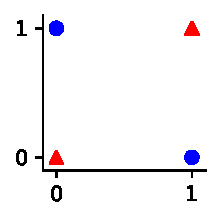
\includegraphics{figures/chapter1/xor_function.pdf}
  \caption{Graphical representation of the XOR function. This function cannot be separated by a linear classifier.}
  \label{figure:xor_function}
\end{figure}
To circumvent these limitations, \citet{minsky1969perceptrons} considered that \emph{another layer of logic} could be added to the function allowing the classification to be done on another representation (see Figure~\ref{figure:multi_layer_perceptron}).
Let $\phi_1$ and $\phi_2$ be two linear functions, we could define a \emph{Multi-Layer Perceptron} as follows:
\begin{equation}
  f(\xvec) = \rho \circ \phi_2 \circ \rho \circ \phi_1( \xvec )
\end{equation}

\begin{figure}[ht]
  \centering
  \begin{subfigure}[t]{0.30\textwidth}
    \centering
    \begin{tabular}{c|c}
      \multicolumn{2}{c}{$\xvec$} \\
      \midrule
      0 & 0 \\
      0 & 1 \\
      1 & 0 \\
      1 & 1
    \end{tabular} 
    \caption*{Input representation}
  \end{subfigure}
  \begin{subfigure}[t]{0.03\textwidth}
    $\rightarrow$
  \end{subfigure}
  \begin{subfigure}[t]{0.30\textwidth}
    \centering
    \begin{tabular}{C{0.5cm} | C{0.5cm}}
      \multicolumn{2}{c}{$\rho \circ \phi_1(\xvec)$} \\
      \midrule
      0 & 0 \\
      0 & 1 \\
      1 & 0 \\
      0 & 0
    \end{tabular}
    \caption*{Intermediate representation}
  \end{subfigure}
  \begin{subfigure}[t]{0.03\textwidth}
    $\rightarrow$
  \end{subfigure}
  \begin{subfigure}[t]{0.30\textwidth}
    \centering
    \begin{tabular}{c}
      $f(\xvec)$ \\
      \midrule
      0 \\
      1 \\
      1 \\
      0
    \end{tabular}
    \caption*{Final representation}
  \end{subfigure}
  \caption{Classification of the XOR function with a Multi-Layer Perceptron}
  \label{figure:multi_layer_perceptron}
\end{figure}

One of the first \emph{Multi-Layer Perceptron}, or now more commonly known as \emph{Deep Neural Network}, was introduced by~\citeauthor{ivakhnenko1967cybernetics} in~\citeyear{ivakhnenko1967cybernetics}.
More precisely, a Neural Neural can be analytically described as a composition of linear functions interlaced with non-linear functions (also called activation functions):
\begin{equation}
  f_\Theta(\xvec) = \phi_{\Wmat_p} \circ \rho \circ \phi_{\Wmat_{p-1}} \circ \cdots \circ \phi_{\Wmat_2} \circ \rho \circ \phi_{\Wmat_1}(\xvec)
  \label{equation:neural_network}
\end{equation}
where the function $\phi_{\Wmat_i}$ is a linear function parameterized by $\Wmat_i$, $\rho$ is a non-linear function, $\Theta \triangleq ( \Wmat_1, \dots, \Wmat_p )$ and $p$ correspond to the \emph{depth} of the network (\ie, the number of layers).
If the weight matrices are dense, this architecture is called \emph{Fully Connected Neural Network} because all the neurons from the first activation are connected to all the neurons from the second activation.

Therefore, a neural network is a function $f_\Theta:\Rbb^n \rightarrow \Rbb^m$ parameterized by weights and composed of at least two linear functions (layers) and one non-linear function (activation function).
The input space $n$ is usually large and the output space $m$ corresponds to the number of classes the network has to classify; therefore, we have $m \ll n$.
In the supervised learning framework, the hypothesis space becomes the set of neural networks parameterized by $\Theta$: $\mathcal{H} = \left\{ f_\Theta \ |\ \Theta = ( \Wmat_1, \dots, \Wmat_p ) \right\}$,
% \begin{equation}
%   \mathcal{H} = \left\{ f_\Theta \ |\ \Theta = \{ \Wmat_1, \dots, \Wmat_p \} \right\} ,
% \end{equation}
then the learning procedure can be taken over $\Theta$ as follows:
\begin{equation}
  \hat{f}^* = \argmin_{\Theta} E(f_\Theta, n) 
\end{equation}



% If $f:\Rbb^n \rightarrow \Rbb^m$ is a two layers neural network:
% \begin{equation}
%   f(\xvec) = \Wmat_2 \rho(\Wmat_1 \xvec)
%   \label{equation:two_layer_neural_network}
% \end{equation}
% where $\Wmat_1 \in \Rbb^{n \times n}$, $\Wmat_2 \in \Rbb^{m \times n}$ are dense matrices.
% This architecture is called \emph{Fully Connected Neural Network} because all the neurons from the first activation are connected to all the neurons from the second activation.

% This type of network can have a large number of parameters, 



%%%%%%%%%%%%%%%%%%%%%%%%%%%%%%%%%%%%%%%%%%%%%%%%%%%%%%%%%%%%%%%%%%%%%%%%%%%%%%%
\section{Introducing Structure into Deep Neural Networks}
\label{section:ch1-introducting_structure_into_deep_neural_networks}
%%%%%%%%%%%%%%%%%%%%%%%%%%%%%%%%%%%%%%%%%%%%%%%%%%%%%%%%%%%%%%%%%%%%%%%%%%%%%%%


Fully connected neural networks can have a very large number of parameters with respect to the number of data points used in real-world datasets.
For example, with the MNIST dataset~\cite{lecun1998gradient} which consists of $5 \times 10^4$ images of handwritten digits from 0 to 9, a two-layer fully connected neural network will have more than $6 \times 10^5$ parameters.
Training such a large network has a number of significant drawbacks: they are hard to train, subject to overfitting and are computationally expensive.
To overcome these limitations, \citet{vapnik1992principles} have proposed to replace the empirical risk minimization principle by \emph{structural risk minimization} (SRM) which consists of implementing ERM with the addition of a structure on the hypothesis space.
Adding a structure on the hypothesis space can be done using two methods: constraining the architecture of the network, constraining the learning procedure by adding a regularization term. 
Hereafter, we present in more detail the two approaches.  

% \begin{itemize}
%   \item reducing the number of parameters by introducing structure into the architecture;
%   \item constraining the learning procedure by adding a regularization term.
% \end{itemize}


% In recent years, Deep Neural Networks have achieved state-of-the-art performances in a variety of domains such as image recognition~\cite{lecun1998gradient,krizhevsky2012imagenet,He_2016_CVPR,tan2019efficientnet}, object detection~\cite{redmon2016you}, natural language processing~\cite{radford2018Language, xxx}, speech recognition~\cite{hinton2012deep, xxx}, etc. 
% This success is mostly due to the advent of specific architectures and learning procedure devised for each applications.  

% However, in order for Deep Neural Networks to achieve such performance, specific architectures and learning procedure have been devised for each application. 
% % More precisely, each of these architectures relies on specific \emph{structured linear transformations}.
%
% In this setting, a phenomenon called overfitting can arise. 
%
% To overcome these limitations,
%
% have proposed two methods to overcome these limitations. 



% \paragraph{Structural Risk Minimization} (SRM).
% The ERM principle assumes that the function $\hat{h}^*$ minimizing $E(h, n)$ leads to the risk $R(\hat{h}^*)$ being close to the minimum.
% This assumption mean that as the \emph{size} of the training set increase the minimization becomes more accurate. More formally, the ERM principle assumes that $R(\hat{h}^*)$ converge to its minimum value on the set $h \in \mathcal{H}$ when $n \rightarrow \infty$.  
% \citet{Vapnik1991TheNA} have shown that this equivalent to say that the empirical risk $E(h, n)$ \emph{converge uniformly} to the actual risk $R(h)$ over $h \in \mathcal{H}$ where the \emph{uniform convergence} is defined as follows:
% \begin{equation}
%   \Pbb \left[ \sup_{h \in \mathcal{H}} \left| R(h) - E(h, n) \right| < \epsilon \right] \rightarrow 0 \quad \text{ when } \quad n \rightarrow \infty, \quad \forall \epsilon > 0 
% \end{equation}

%%%%%%%%%%%%%%%%%%%%%%%%%%%%%%%%%%%%%%%%%%%%%%%%%%%%%%%%%%%%%%%%%%%%%%%%%%%%%%%
\subsection{Structure Given by the Architecture of the Neural Network}
\label{subsection:ch1-introducing_structured_into_the_architecture_of_neural_networks}
%%%%%%%%%%%%%%%%%%%%%%%%%%%%%%%%%%%%%%%%%%%%%%%%%%%%%%%%%%%%%%%%%%%%%%%%%%%%%%%

% In recent years, Deep Neural Networks have achivied state-of-the-art results on computer vision tasks 
%
% In recent years, Deep Neural Networks have achieved state-of-the-art performances in a variety of domains such as image recognition (LeCun et al. 1998; Krizhevsky, Sutskever et al. 2012; He et al. 2016; Tan & Le, 2019), image detection (Redmon et al. 2016), natural language processing (Radford et al. 2018), speech recognition Hinton et al. (2012), etc. 
%
% In order for Deep Neural Networks to achieve such performance, specific architectures have been devised for each application. More precisely, each of these architectures relies on specific structured linear transformations.

\begin{figure}[htb]
  \centering
  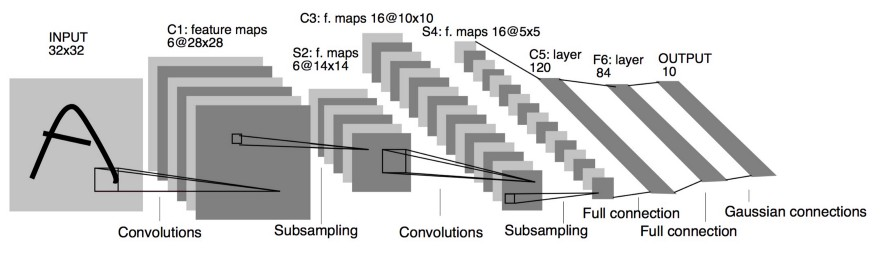
\includegraphics[scale=0.4]{figures/chapter1/lenet.jpg}
  \caption{Graphical representation of the LeNet architecture proposed by \citet{lecun1998gradient}}
  \label{figure:lenet_network}
\end{figure}

A perfect example of neural networks with a specific architecture are \emph{Convolutional Neural Networks} (CNN)~\cite{lecun1998gradient,krizhevsky2012imagenet,He_2016_CVPR,tan2019efficientnet} which consists of neural networks with specific structured linear transformations. 
The structured linear transform used in convolutional layers is the discrete convolution which consists of a kernel sliding over the image and acting as a filter.
% A perfect example of such efficient linear operation is the discrete convolution which consists of a kernel sliding over the image and acting as a filter.
Let $\avec$ and $\bvec$ be two vectors indexed by the set $M = \{-m, -m+1, \dots, m-1, m\}$, the discrete convolution between the signals $\avec$ and $\bvec$ is given by: 
\begin{equation}
  (\avec \ast \bvec) \left[ n \right] \triangleq \sum_{m \in M} \avec\left[m\right] \cdot \bvec\left[n - m\right]
\end{equation}
The convolution operation has translation invariance characteristics \cite{zhang1990parallel} which is perfectly suited for image classification (objects can be at different positions in images).  
\citet{lecun1998gradient} was one of the first to successfully train a convolutional neural network, achieving state-of-the-art performance on the MNIST dataset.
Convolution neural networks achieve such a great result for two main reasons:
first, CNNs are similar to the connectivity pattern of neurons in the visual cortex of the human brain. 
Secondly, CNNs are very efficient due to the sharing of parameters. 
While a classical linear operation with dense matrix has $n \times n$ parameters, a convolution only has $k \times k$ parameters where $k$ is the kernel size and is usually small (\eg 3 or 5 for classical convolution layers use in neural networks).
This weight sharing reduces the number of weights with respect to the fully connected neural network. The LeNet architecture (see Figure~\ref{figure:lenet_network}) has only $6 \times 10^4$ parameters.  


Although, convolutional neural networks perform well on specific tasks, important questions remain on the architecture of neural networks. 
% Which structure is better suited for neural networks?
Can we use other types of structure for neural networks?  
Does the reduction of parameters reduce the performance of the network?


%%%%%%%%%%%%%%%%%%%%%%%%%%%%%%%%%%%%%%%%%%%%%%%%%%%%%%%%%%%%%%%%%%%%%%%%%%%%%%%
\subsection{Structure Given by the Learning Procedure}
\label{subsection:ch1-introducing_structured_into_the_learning_procedure}
%%%%%%%%%%%%%%%%%%%%%%%%%%%%%%%%%%%%%%%%%%%%%%%%%%%%%%%%%%%%%%%%%%%%%%%%%%%%%%%

Instead of constraining the architecture of the network, we can constrain the learning procedure in order to reduce to search space.
Consider the following hypothesis space $\mathcal{H} = \left\{ f_\Theta \ |\ \Theta = ( \Wmat_1, \cdots, \Wmat_p ) \right\}$ which define the set of neural networks with fixed architecture.
We can introduce a structure in the hypothesis space by setting:
\begin{equation}
  \mathcal{H} = \left\{ f_\Theta \ |\ \Theta = ( \Wmat_1, \cdots, \Wmat_p ) \ |\ R(\Theta) \right\} 
\end{equation}
where $R(\Theta)$ is a constrain on $\Theta$ called a regularizer.
One of the most common form of regularization consists of adjusting the weights during the learning procedure under the constraint to keep the magnitude of the weights small.
This regularization has been introduced by~\citet{tikhonov_arsenin_1977} and is commonly known as \emph{weight decay}.
With this constraint, the hypothesis space can be defined as follows:
\begin{equation}
  \mathcal{H_\epsilon} = \left\{ f_\Theta \ |\ \Theta = (\Wmat_1, \cdots, \Wmat_p) \ | \ \norm{\Wmat_i}_\mathrm{F} \leq \epsilon \right\} 
\end{equation}
For a convex loss function, the minimization of the empirical risk within the set $\mathcal{H}_\epsilon$ can be achieved with the minimization of
\begin{equation}
  E(f_\Theta, n, \lambda) = \frac{1}{n} \sum_{i = 1}^{n} L\left(f_\Theta(\xvec^{(i)}), y^{(i)} \right) + \lambda \sum_{i = 1}^{p} \norm{\Wmat_i}_\mathrm{F}
\end{equation}
where $\lambda$ is a Lagrange multiplier.

Defining a regularization strategy is still an open problem in supervised learning. Recent works have proposed different form of regularization.  











%
%
% The concept of \emph{supervised learning} which refers to the notion of learning the parameters of a specific function (neural network) that maps an input to an output based on example input-output pairs.
% For example, an image (input) associated with its content: label (output).
% The steps of the learning procedure are as follows. 
% First, a neural network is initialized with random weights.
% Then, the algorithm \emph{analyzed} the training dataset and \emph{adjust} the weights in order for the network to correctly map the input to the output. 
%
% Due to the important expressivity of neural networks and of the finite number of sample data point, the learning procedure can produce a learned neural network that fits to closely on the training dataset and fail to fit on unseen example.
% This phenomenon is called \emph{overfitting} and can significantly decrease the general performance of neural networks.
% In order to limit overfitting and improve the general performance of neural network, \citet{vapnik1992principles} have proposed to constraint the learning procedure by adding a regularization term.  



% Another method proposed by \cite{vapnik1992principles} is to constraint the learning procedure in order to improve the performance of neural networks. 
%
% Important questions remain on supervised learning algorithms:
% Which properties can we leverage from these structures to improve the training and performance of neural networks? 


% Overfitting is a modeling error that occurs when a function is too closely fit to a limited set of data points. Overfitting the model generally takes the form of making an overly complex model to explain idiosyncrasies in the data under study.


% The choice of the function used for supervised learning is an active area of research and will be part of the focus of this thesis.
% In this work, we study \emph{neural networks} which are a class of function widely used for unstructured datasets (image, sound, text).






%%%%%%%%%%%%%%%%%%%%%%%%%%%%%%%%%%%%%%%%%%%%%%%%%%%%%%%%%%%%%%%%%%%%%%%%%%%%%%%
\section{Main contributions and Outline of the Thesis}
\label{section:ch1-main_contributions_and_outline_of_the_thesis}
%%%%%%%%%%%%%%%%%%%%%%%%%%%%%%%%%%%%%%%%%%%%%%%%%%%%%%%%%%%%%%%%%%%%%%%%%%%%%%%

%%%%%%%%%%%%%%%%%%%%%%%%%%%%%%%%%%%%%%%%%%%%%%%%%%%%%%%%%%%%%%%%%%%%%%%%%%%%%%%
\subsection{Main Contributions}
\label{subsection:ch1-main_contributions}
%%%%%%%%%%%%%%%%%%%%%%%%%%%%%%%%%%%%%%%%%%%%%%%%%%%%%%%%%%%%%%%%%%%%%%%%%%%%%%%

In this thesis, we leverage the properties of \emph{structured matrices} for the problems mentioned in Section~\ref{subsection:ch1-introducing_structured_into_the_architecture_of_neural_networks} and \ref{subsection:ch1-introducing_structured_into_the_learning_procedure}. A $n \times n$ structure matrix can be represented with less than $n^2$ parameters, Figure~\ref{figure:example_structure_matrices} shows an example of structured matrices.
In addition to offering a more compact representation, the structure of certain matrices can be leveraged to obtain better algorithms for matrix-vector product leading in memory and computationally operations. 

\begin{figure}[ht]
   \centering
   \begin{subfigure}[t]{0.24\textwidth}
       \centering
       \begin{equation*}
	  \leftmatrix
	    a &   &   &   \\
	      & b &   &   \\
	      &   & c &   \\
	      &   &   & d
	  \rightmatrix
       \end{equation*}
       \caption*{diagonal}
   \end{subfigure}
   \hfill
   \begin{subfigure}[t]{0.24\textwidth}
       \centering
       \begin{equation*}
	  \leftmatrix
	    a & b & c & d \\
	    e & a & b & c \\
	    f & e & a & b \\
	    d & f & e & a
	  \rightmatrix
       \end{equation*}
       \caption*{Toeplitz}
   \end{subfigure}
   \hfill
   \begin{subfigure}[t]{0.24\textwidth}
       \centering
       \begin{equation*}
	  \leftmatrix
	    ae & af & ag & ah \\
	    be & bf & bg & bh \\
	    ce & cf & cg & ch \\
	    de & df & dg & dh
	  \rightmatrix
       \end{equation*}
       \caption*{Low Rank}
   \end{subfigure}
   \hfill
   \begin{subfigure}[t]{0.24\textwidth}
       \centering
       \begin{equation*}
	  \leftmatrix
	    a & a^2 & a^3 & a^4 \\
	    b & b^2 & b^3 & b^4 \\
	    c & c^2 & c^3 & c^4 \\
	    d & d^2 & d^3 & d^4
	  \rightmatrix
       \end{equation*}
       \caption*{Vandermonde}
   \end{subfigure}
  \caption{Examples of structured matrices.}
  \label{figure:example_structure_matrices}
\end{figure}

More specifically, we study the proprieties of structured matrices from the Toeplitz family to make two contributions presented below:

\paragraph{Contribution 1} (C1)
We use circulant matrices, which are a particular case of Toeplitz matrices, to devise a new compact architecture replacing Fully Connected Neural Networks.
More precisely, we study deep diagonal circulant neural networks, which are deep neural networks in which weight matrices are the product of diagonal and circulant ones.
Besides making a theoretical analysis of their expressivity, we introduce principled techniques for training these models: we devise an initialization scheme and propose a smart use of non-linearity functions in order to train deep diagonal circulant networks. 
Furthermore, we show that these networks outperform recently introduced deep networks with other types of structured layers.
We conduct a thorough experimental study to compare the performance of deep diagonal circulant networks with state-of-the-art models based on structured matrices and with dense models.
We show that our models achieve better accuracy than other structured approaches while requiring 2x fewer weights than the next best approach.
Finally, we train compact and accurate deep diagonal circulant networks on a real-world video classification dataset with over 3.8 million training examples. 

\paragraph{Contribution 2} (C2)
It is well known that a discrete convolution operation with a 2d kernel applied on a 2d signal is equivalent to a matrix multiplication with a doubly-block Toeplitz matrix~\cite{jain1989fundamentals} (see Appendix~\ref{xxx}). 
Based on this knowledge and by leveraging the theory of Toeplitz matrices, we introduce a new upper bound on the Lipschitz constant for convolutional layers that is both tight and easy to compute.
This bound allows us to tackle the problem of Lipschitz regularization of Convolutional Neural Networks which is established now established as a key property of modern deep learning with implications in training stability, generalization, robustness against adversarial examples, etc.

% we leverage the properties of doubly-block Toeplitz matrices to devised a new fast and efficient method to compute the Lipschitz constant of convolutional layers. 
%
% However, computing the exact value of the Lipschitz constant of a neural network is known to be NP-hard.
% Recent attempts from the literature introduce upper bounds to approximate this constant that are either efficient but loose or accurate but computationally expensive.
% In this work, Based on this result we devise an algorithm to train Lipschitz regularized Convolutional Neural Networks.
%
% The contributions of this Thesis are based on structured matrices from the Toeplitz family.
%
% More specifically, in Chapter~\ref{chapter:diagonal_circulant_neural_network}, In Chapter~\ref{chapter:lipschitz_bound}, we leverage the structure of convolutional layers to devise a new regularization scheme for neural networks. 


%%%%%%%%%%%%%%%%%%%%%%%%%%%%%%%%%%%%%%%%%%%%%%%%%%%%%%%%%%%%%%%%%%%%%%%%%%%%%%%
\subsection{Outline of the Thesis}
\label{subsection:ch1-outline_of_the_thesis}
%%%%%%%%%%%%%%%%%%%%%%%%%%%%%%%%%%%%%%%%%%%%%%%%%%%%%%%%%%%%%%%%%%%%%%%%%%%%%%%

\todo{update this paragraph at the end of the writing}

% The thesis is organized as follows. The first Chapter (Chapter~\ref{chapter:related_work}) is dedicated to enumerating state-of-the-art approaches on both contributions. In a first part, we review approaches on compact neural networks. In a second part, we review  
%
% Chapter~\ref{chapter:related_work} present a related work in two parts: first we review existing techniques for on building compact neural network architecture. Then, we present different techniques to constraint the learning procedure. 
%
% The following two chapters contains the main contributions of the Thesis.  
% Finally, Chapter~\ref{chapter:conclusion} provides concluding remarks and a discussion.



  % 
%%%%%%%%%%%%%%%%%%%%%%%%%%%%%%%%%%%%%%%%%%%%%%%%%%%%%%%%%%%%%%%%%%%%%%%%%%%%%%%
\chapter{Related Work}
\label{chapter:related_work}
%%%%%%%%%%%%%%%%%%%%%%%%%%%%%%%%%%%%%%%%%%%%%%%%%%%%%%%%%%%%%%%%%%%%%%%%%%%%%%%
\localtableofcontents


%%%%%%%%%%%%%%%%%%%%%%%%%%%%%%%%%%%%%%%%%%%%%%%%%%%%%%%%%%%%%%%%%%%%%%%%%%%%%%%
\section{Introduction}
\label{section:ch2-introduction}
%%%%%%%%%%%%%%%%%%%%%%%%%%%%%%%%%%%%%%%%%%%%%%%%%%%%%%%%%%%%%%%%%%%%%%%%%%%%%%%

The problems addressed in this thesis are from the field of \emph{supervised} machine learning and \emph{neural networks}.  
As stated in Chapter~\ref{chapter:introduction}, fully connected neural networks learned with the empirical risk minimization principle can be hard to train and subject to overfitting.
The common denominator of these problems is the very large number of parameters used in fully connected neural networks.  
To overcome these challenges, \citet{vapnik1992principles} have proposed to replaced the ERM principle by the \emph{structural risk minimization} procedure.
Structural risk minimization can be implemented using two methods as stated in the work 
\begin{enumerate}
  \item designing compact neural network architecture in order to reduce the number of parameters;
  \item constraining the hypothesis space with a \emph{regularization} in order to reduce the search space of the learning procedure.
\end{enumerate}
Both methods introduce \emph{structure} on the set of functions implemented by neural networks. 

In this thesis, by leveraging the properties of matrices from the Toeplitz family, we contribute of designing and better understanding a new neural network architecture based on circulant and diagonal matrices. 


%%%%%%%%%%%%%%%%%%%%%%%%%%%%%%%%%%%%%%%%%%%%%%%%%%%%%%%%%%%%%%%%%%%%%%%%%%%%%%%
\subsection{Theoretical Intuition Behind Structural Risk Minimization}
\label{subsection:ch2-xxx}
%%%%%%%%%%%%%%%%%%%%%%%%%%%%%%%%%%%%%%%%%%%%%%%%%%%%%%%%%%%%%%%%%%%%%%%%%%%%%%%

The ERM principle assumes that the function $\hat{h}^*$ minimizing $E(h, n)$ leads to the risk $R(\hat{h}^*)$ being close to the minimum.
This assumption mean that as the \emph{size} of the training set increase the minimization becomes more accurate. More formally, the ERM principle assumes that $R(\hat{h}^*)$ converge to its minimum value on the set $h \in \mathcal{H}$ when $n \rightarrow \infty$.  
\citet{Vapnik1991TheNA} have shown that this equivalent to say that the empirical risk $E(h, n)$ \emph{converge uniformly} to the actual risk $R(h)$ over $h \in \mathcal{H}$ where the \emph{uniform convergence} is defined as follows:
\begin{equation}
  \Pbb \left[ \sup_{h \in \mathcal{H}} \left| R(h) - E(h, n) \right| < \epsilon \right] \rightarrow 0 \quad \text{ when } \quad n \rightarrow \infty, \quad \forall \epsilon > 0 
\end{equation}


The study of uniform convergence of empirical risk to actual risk has become one of the important problems of Machine Learning Theory over the last 40 years \cite{}.
This study includes a description of necessary and sufficient conditions as well as bounds for the rate of convergence \cite{vapnik1982estimation}. 




The theory of uniform convergence O


It would be of interest to bound the 



\begin{equation}
  \Pbb \left[ \sup_{h \in \mathcal{H}} \left| R(h) - E(h, n) \right| < \epsilon \right] \leq \left( \frac{2 n e}{\mu} \right)^\mu \exp\{ -\epsilon ^2 n\} 
\end{equation}







%%%%%%%%%%%%%%%%%%%%%%%%%%%%%%%%%%%%%%%%%%%%%%%%%%%%%%%%%%%%%%%%%%%%%%%%%%%%%%%
\subsection{Outline of the Chapter}
\label{subsection:ch2-outline_of_the_chapter}
%%%%%%%%%%%%%%%%%%%%%%%%%%%%%%%%%%%%%%%%%%%%%%%%%%%%%%%%%%%%%%%%%%%%%%%%%%%%%%%

\todo{write this outline at the end of the writing}

In this chapter we review state-of-the-art approaches on these two methods. 







%%%%%%%%%%%%%%%%%%%%%%%%%%%%%%%%%%%%%%%%%%%%%%%%%%%%%%%%%%%%%%%%%%%%%%%%%%%%%%%
\section{Structure given by the learning procedure}
\label{section:ch2-xxx}
%%%%%%%%%%%%%%%%%%%%%%%%%%%%%%%%%%%%%%%%%%%%%%%%%%%%%%%%%%%%%%%%%%%%%%%%%%%%%%%


%%%%%%%%%%%%%%%%%%%%%%%%%%%%%%%%%%%%%%%%%%%%%%%%%%%%%%%%%%%%%%%%%%%%%%%%%%%%%%%
\section{Lipschitz Regularization of Neural Networks}
\label{section:ch5-related_work}
%%%%%%%%%%%%%%%%%%%%%%%%%%%%%%%%%%%%%%%%%%%%%%%%%%%%%%%%%%%%%%%%%%%%%%%%%%%%%%%

A popular technique for approximating the maximal singular value of a matrix is the power method~\cite{golub2000eigenvalue}, an iterative algorithm which yields a good approximation of the maximum singular value when the algorithm is able to run for a sufficient number of iterations. 
\citet{yoshida2017spectral, miyato2018spectral} have used the power method to normalize the spectral norm of each layer of a neural network, and showed that the resulting models offered improved generalization performance and generated better examples when they were used in the context of GANs. 
\citet{farnia2018generalizable} built upon the work of~\citet{miyato2018spectral} and proposed a power method specific for convolutional layers that leverages the deconvolution operation and avoid the computation of the gradient.
They used it in combination with adversarial training. 
In the same vein, \citet{gouk2018regularisation} demonstrated that regularized neural networks using the power method also offered improvements over their non-regularized counterparts. 
Furthermore, \citet{tsuzuku2018lipschitz} have shown that a neural network can be more robust to some adversarial attacks, if the prediction margin of the network (\ie the difference between the first and the second maximum logit) is higher than a minimum threshold that depends on the global Lipschitz constant of the network.
Building on this observation, they use the power method to compute an upper bound on the global Lipschitz constant, and maximize the prediction margin during training.
Finally, \citet{scaman2018lipschitz} have used automatic differentiation combined with the power method to compute a tighter bound on the global Lipschitz constant of neural networks.
Despite a number of interesting results, using the power method is expensive and results in prohibitive training times. 

Other approaches to regularize the Lipschitz constant of neural networks have been proposed by~\citet{sedghi2018singular} and~\citet{singla2019bounding}.
The method of~\citet{sedghi2018singular} exploits the properties of circulant matrices to approximate the maximal singular value of a convolutional layer.
Although interesting, this method results in a loose approximation of the maximal singular value of a convolutional layer.
Furthermore, the complexity of their algorithm is dependent on the convolution input which can be high for large datasets such as ImageNet.
More recently, \citet{singla2019bounding} have successfully bounded the operator norm of the Jacobian matrix of a convolution layer by the Frobenius norm of the reshaped kernel.
This technique has the advantage to be very fast to compute and to be independent of the input size but it also results in a loose approximation. 

To build robust neural networks, \citet{cisse2017parseval} and ~\citet{NIPS2019_9673} have proposed to constrain the Lipschitz constant of neural networks by using orthogonal convolutions.
\citet{cisse2017parseval} use the concept of \emph{parseval tight frames}, to constrain their networks.
\citet{NIPS2019_9673} built upon the work of~\citet{cisse2017parseval} to propose an efficient construction method of orthogonal convolutions.  

Finally, recent work~\citet{NIPS2019_9319,latorre2020lipschitz} has proposed a tight bound on the Lipschitz constant of the full network with the use of semi-definite programming.
These works are theoretically interesting but lack scalability (\ie the bound can only be computed on small networks).




  %%%%%%%%%%%%%%%%%%%%%%%%%%%%%%%%%%%%%%%%%%%%%%%%%%%%%%%%%%%%%%%%%%%%%%%%%%%%%%%
\chapter{Diagonal Circulant Neural Networks}
\label{chapter:diagonal_circulant_neural_network}
%%%%%%%%%%%%%%%%%%%%%%%%%%%%%%%%%%%%%%%%%%%%%%%%%%%%%%%%%%%%%%%%%%%%%%%%%%%%%%%
\localtableofcontents

% \begin{abstract}
% In this paper, we study deep diagonal circulant neural networks, which are deep neural networks in which weight matrices are the product of diagonal and circulant ones.
% Besides making a theoretical analysis of their expressivity, we introduce principled techniques for training these models: we devise an initialization scheme and propose a smart use of non-linearity functions in order to train deep diagonal circulant networks. 
% Furthermore, we show that these networks outperform recently introduced deep networks with other types of structured layers. We conduct a thorough experimental study to compare the performance of deep diagonal circulant networks with state-of-the-art models based on structured matrices and with dense models. We show that our models achieve better accuracy than other structured approaches while requiring 2x fewer weights than the next best approach. Finally, we train compact and accurate deep diagonal circulant networks on a real world video classification dataset with over 3.8 million training examples. 
% \end{abstract}


% ##############################################################################
\section{Introduction}
\label{introduction}
% ##############################################################################


The deep learning revolution has yielded models of increasingly large size. 
In recent years, designing compact and accurate neural networks with a small number of trainable parameters has been an active research topic.
It is motivated by practical applications in embedded systems (to reduce memory footprint \cite{43969}), federated and distributed learning (to reduce communication \cite{45648}), derivative-free optimization in reinforcement learning (to simplify the computation of the approximated gradient \cite{47028}), etc.
Besides a number of practical applications, it is also an important research question whether or not models really need to be this large or if smaller networks can achieve similar accuracy~\cite{ba2014deep}.

Structured matrices are at the very core of most of the work on compact networks.
In these models, dense weight matrices are replaced by matrices with a prescribed structure (\emph{low rank matrices, Toeplitz matrices, circulant matrices, LDR, etc.}).
Despite substantial efforts \cite{cheng,moczulski2015acdc}, the performance of compact models is still far from achieving an acceptable accuracy motivating their use in real-world scenarios.
This raises several questions about the effectiveness of such models and about our ability to train them. In particular two main questions call for investigation:
\begin{itemize}
  \item[] \textbf{Q1} \emph{How to efficiently train deep neural networks with a large number of structured layers?}
  \item[] \textbf{Q2} \emph{What is the expressive power of structured layers compared to dense layers?}
\end{itemize}


In this paper, we provide principled answers to these questions for the particular case of deep neural networks based on diagonal and circulant matrices (\aka Diagonal-circulant neural networks or DCNNs). 

The idea of using diagonal and circulant matrices together comes from a series of results in linear algebra by \citet{muller1998algorithmic} and \citet{Huhtanen2015}.
The most recent result from \citet{Huhtanen2015} demonstrates that any matrix $\Amat \in \Cnn$ can be decomposed into the product of $2n-1$ alternating diagonal and circulant matrices.
The diagonal-circulant decomposition inspired \citet{moczulski2015acdc} to design the \emph{Structured Efficient Linear Layers} (SELL), which is the building block of DCNNs.
However, they were not able to train deep neural networks based on these layers. 

To answer \textbf{Q1}, we first describe a theoretically sound initialization procedure for DCNN which allows the signal to propagate through the network without vanishing or exploding.
Furthermore, we provide a number of empirical insights to explain the behaviour of DCNNs and show the impact of the number of the non-linearities in the network on the convergence rate and the accuracy of the network. 
By combining all these insights, we are able (for the first time) to train large and deep DCNNs and demonstrate the good performance of these networks on a large scale application (the \yt video classification problem) and obtain very competitive accuracy. 

To answer \textbf{Q2}, we propose an analysis of the expressivity of DCNNs by extending the results by \citet{Huhtanen2015}.
We introduce a new bound on the number of diagonal-circulant products required to approximate a matrix that depends on its rank.
Building on this result, we demonstrate that a DCNN with bounded width and small depth can approximate any dense networks with ReLU activations. 

\paragraph{Outline of the chapter:}
We present in Section~\ref{section:ch3-related_work} the related work on structured neural networks and several compression techniques.
Section~\ref{section:circulant} introduces circulant matrices, our new result extending the one from \citet{Huhtanen2015}.
Section~\ref{section:analysis_diagonal_circulant} proposes a theoretical analysis on the expressivity on DCNNs.
Section~\ref{section:training} describes two efficient techniques for training deep diagonal circulant neural networks.
Finally, Section~\ref{section:empirical_evaluation} presents extensive experiments to compare the performance of deep diagonal circulant neural networks in different settings with respect to other state of the art approaches.
Section~\ref{section:ch3-conclusion} provides a discussion and concluding remarks.


% #############################################################################
\section{Related Work}
\label{section:ch3-related_work}
% #############################################################################

Structured matrices exhibit a number of good properties which have been exploited by deep learning practitioners, mainly to compress large neural networks architectures into smaller ones.
For example, \citet{hinrichs2011johnson} have demonstrated that a single circulant matrix can be used to approximate the Johnson-Lindenstrauss transform, often used in machine learning to perform dimensionality reduction.
Building upon this result, \citet{cheng} proposed to replace the weight matrix of a fully connected layer by a circulant matrix effectively replacing the complex transform modeled by the fully connected layer by a simple dimensionality reduction.
Despite the reduction of expressivity, the resulting network demonstrated good accuracy using only a fraction of its original size (90\% reduction).


\paragraph{Comparison with \ACDC.}
\citet{moczulski2015acdc} have introduced two \emph{Structured Efficient Linear Layers} (SELL) called \AFDF and \ACDC, where $\Amat$ and $\Dmat$ are diagonal matrices and $\Fmat$ and $\Cmat$ are the Fourier and cosine transform respectively.
The \AFDF structured layer benefits from the theoretical results introduced by \citet{Huhtanen2015} and can be seen as the building block of DCNNs.
However, \citet{moczulski2015acdc} only experiment using \ACDC, a different type of layer that does not involve circulant matrices.
As far as we can tell, the theoretical guarantees available for the \AFDF layer do not apply on the \ACDC layer since the cosine transform does not diagonalize circulant matrices \cite{sanchez1995diagonalizing}.
Another possible limit of the \ACDC paper is that they only train large neural networks involving \ACDC layers combined with many other expressive layers.
Although the resulting network demonstrates good accuracy, it is difficult the characterize the true contribution of the \ACDC layers in this setting. 

\paragraph{Comparison with Low displacement rank structures.}
More recently, \citet{Thomas_NIPS2018_8119} have generalized these works by proposing neural networks with low-displacement rank matrices (LDR), that are structured matrices encompassing a large family of structured matrices, including Toeplitz-like, Vandermonde-like, Cauchy-like and more notably DCNNs.
To obtain this result, LDR represents a structured matrix using two displacement operators and a low-rank residual.
Despite being elegant and general, we found that the LDR framework suffers from several limits which are inherent to its generality and makes it difficult to use in the context of large and deep neural networks.
First, the training procedure for learning LDR matrices is highly involved and implies many complex mathematical objects such as Krylov matrices.
Then, as acknowledged by the authors, the number of parameters required to represent a given structured matrix (a \emph{Toeplitz matrix}) in practice is unnecessarily high (higher than required in theory). 

\paragraph{Other compression techniques.}
Besides structured matrices, a variety of techniques have been proposed to build more compact deep learning models.
These include \emph{model distillation}~\cite{44873}, Tensor Train~\cite{novikov2015tensorizing}, Low-rank decomposition~\cite{NIPS2013_5025}, to mention a few.
However, circulant networks show good performances in several contexts (the interested reader can refer to the results reported by \citet{moczulski2015acdc} and \citet{Thomas_NIPS2018_8119}).


% #############################################################################
\section{A Primer on Circulant Matrices and a New Result}
\label{section:circulant}
% #############################################################################

An $n$-by-$n$ circulant matrix $\Cmat$ is a matrix where each row is a cyclic right shift of the previous one as illustrated below.

\begin{equation}
    \Cmat = \circulant(\cvec) = \leftmatrix
    c_{0} & c_{n-1} & c_{n-2} & \dots & c_{1} \\
    c_{1} & c_{0} & c_{n-1} & & c_{2} \\
    c_{2} & c_{1} & c_{0}& & c_{3} \\
    \vdots & & & \ddots & \vdots \\
    c_{n-1} & c_{n-2} & c_{n-3} & & \phantom{0}c_{0}\phantom{0}
    \rightmatrix
\end{equation}

Circulant matrices exhibit several interesting properties from the perspective of numerical computations.
Most importantly, any $n$-by-$n$ circulant matrix $\Cmat$ can be represented using only $n$ coefficients instead of the $n^2$ coefficients required to represent classical unstructured matrices.
In addition, the matrix-vector product is simplified from $O(n^2)$ to $O(n \log n)$ using the  convolution theorem.

As we will show in this chapter, circulant matrices also have a strong expressive power.
So far, we know that a single circulant matrix can be used to represent a variety of important linear transforms such as random projections~\cite{hinrichs2011johnson}. 
When they are combined with diagonal matrices, they can also be used as building blocks to represent any linear transform~\cite{schmid2000decomposing, Huhtanen2015} with an arbitrary precision.
\citet{Huhtanen2015} were able to bound the number of factors that is required to approximate any matrix $\Amat$ with arbitrary precision.

\paragraph{Relation between diagonal circulant matrices and low rank matrices}
We recall this result in Theorem~\ref{theorem:huhtanen} as it is the starting point of our theoretical analysis.

\begin{theorem}[Reformulation from \citet{Huhtanen2015}] \label{theorem:huhtanen}
  For every matrix $\Amat \in \Cnn$, for any $\epsilon > 0$, there exists a sequence of matrices $\Bmat_1 \ldots \Bmat_{2n-1}$ where $\Bmat_{i}$ is a circulant matrix if $i$ is odd, and a diagonal matrix otherwise, such that $\norm{\Bmat_{1} \Bmat_{2} \ldots \Bmat_{2n-1} - \Amat} < \epsilon$.
\end{theorem}

Unfortunately, this theorem is of little use to understand the expressive power of diagonal-circulant matrices when they are used in deep neural networks.
This is because: 1) the bound only depends on the dimension of the matrix $\Amat$, not on the matrix itself, 2) the theorem does not provide any insights regarding the expressive power of $m$ diagonal-circulant factors when $m$ is much lower than $2n - 1$ as it is the case in most practical scenarios we consider in this chapter. 

In the following theorem, we enhance the result by \citet{Huhtanen2015} by expressing the number of factors required to approximate $\Amat$, \emph{as a function of the rank of $\Amat$}.
This is useful when one deals with low-rank matrices, which is common in machine learning problems. 

\begin{theorem}[Rank-based circulant decomposition] \label{theorem:rank-decomposition}
Let $\Amat \in \Cnn$ be a matrix of rank at most $k$.
Assume that $n$ can be divided by $k$.
For any $\epsilon > 0$, there exists a sequence of $4k+1$ matrices $\Bmat_{1}, \ldots, \Bmat_{4k+1}$, where $\Bmat_{i}$ is a circulant matrix if $i$ is odd, and a diagonal matrix otherwise, such that $\norm{\Bmat_1 \Bmat_2 \ldots \Bmat_{4k+1} - \Amat} < \epsilon$.
\end{theorem}

\begin{proof}[\proofrefth{theorem:rank-decomposition}]
Let $\Umat \mathbf{\Sigma} \Vmat^{T}$ be the SVD decomposition of $\Mmat$ where $\Umat,\Vmat$ and $\mathbf{\Sigma}$ are $n \times n$ matrices.
Because $\Mmat$ is of rank $k$, the last $n-k$ columns of $\Umat$ and $\Vmat$ are null.
In the following, we will first decompose $\Umat$ into a product of matrices $\Wmat\Rmat\Omat$, where $\Rmat$ and $\Omat$ are respectively circulant and diagonal matrices, and $\Wmat$ is a matrix which will be further decomposed into a product of diagonal and circulant matrices.
Then, we will apply the same decomposition technique to $\Vmat$.
Ultimately, we will get a product of $4k+2$ matrices alternatively diagonal and circulant.  

Let $\Rmat = \circulant(r_{1}\ldots r_{n})$. Let $\Omat$ be a $n \times n$ diagonal matrix where $\Omat_{i,i} = 1$ if $i \le k$ and $0$ otherwise. The $k$ first columns of the product $\Rmat\Omat$ will be equal to that of $\Rmat$, and the $n-k$ last colomns of $\Rmat\Omat$ will be zeros. For example, if $k=2$, we have: 
\begin{equation}
  \Rmat\Omat = \leftmatrix
  r_{1} & r_{n} & 0 & \cdots & 0\\
  r_{2} & r_{1}\\
  r_{3} & r_{2} & \vdots &  & \vdots\\
  \vdots & \vdots\\
  r_{n} & r_{n-1} & 0 & \cdots & 0
  \rightmatrix
\end{equation}

Let us define $k$ diagonal matrices $\Dmat_{i} = \diagonal(d_{i1} \ldots d_{in})$ for $i \in [k]$.
For now, the values of $d_{ij}$ are unknown, but we will show how to compute them.
Let $\Wmat = \sum_{i=1}^{k} \Dmat_{i} \Smat^{i-1}$ where $\Smat$ is the \emph{cyclic shift} matrix 
%$S \in \mathbb{R}^{n\times n}$
define as follows:
\begin{equation}
  \Smat = \leftmatrix 0 &  &  &  & 1 \\
  1 & 0 \\
   & 1 & \ddots \\
   &  & \ddots & 0 \\
   &  &  & 1 & 0
  \rightmatrix
\end{equation}


Note that the $n-k$ last columns of the product $\Wmat\Rmat\Omat$ will be zeros.
For example, with $k=2$, we have: 
\begin{equation}
  \Wmat = \leftmatrix
  d_{1,1} &  &  &  & d_{2,1} \\
  d_{2,2} & d_{1,2} \\
   & d_{2,3} & \ddots \\
   &  & \ddots \\
   &  &  & d_{2,n} & d_{1,n}
  \rightmatrix
\end{equation}

\begin{equation}
  \Wmat\Rmat\Omat = \leftmatrix
  r_{1}d_{11}+r_{n}d_{21} & r_{n}d_{11}+r_{n-1}d_{21} & 0 & \cdots & 0 \\
  r_{2}d_{12}+r_{1}d_{22} & r_{1}d_{12}+r_{n}d_{22}\\
   &  & \vdots &  & \vdots \\
  \vdots & \vdots\\
  r_{n}d_{1n}+r_{n-1}d_{2n} & r_{n-1}d_{1n}+r_{n-2}d_{2n} & 0 & \cdots & 0
  \rightmatrix
\end{equation}
We want to find the values of $d_{ij}$ such that $\Wmat \Rmat \Omat = \Umat$. We can formulate this as linear equation system. In case $k=2$, we get:
\begin{equation}
  \leftmatrix
  r_{n} & r_{1}\\
  r_{n-1} & r_{n}\\
   &  & r_{1} & r_{2}\\
   &  & r_{n} & r_{1}\\
   &  &  &  & r_{2} & r_{3}\\
   &  &  &  & r_{1} & r_{2}\\
   &  &  &  &  &  & \ddots\\
   &  &  &  &  &  &  & \ddots
  \rightmatrix \times \leftmatrix
  d_{2,1}\\
  d_{1,1}\\
  d_{2,2}\\
  d_{1,2}\\
  d_{2,3}\\
  d_{1,3}\\
  \vdots\\
  \vdots
  \rightmatrix = \leftmatrix
  \Umat_{1,1}\\
  \Umat_{1,2}\\
  \Umat_{2,1}\\
  \Umat_{2,2}\\
  \\
  \\
  \vdots\\
  \\
  \rightmatrix
\end{equation}

The $i^{th}$ bloc of the bloc-diagonal matrix is a Toeplitz matrix induced by a subsequence of length $k$ of $(r_1,\ldots r_n,r_1 \ldots r_n)$.
Set $r_{j}=1$ for all $j\in\{k,2k,3k,\ldots n\}$ and set $r_{j}=0$ for all other values of $j$.
Then it is easy to see that each bloc is a permutation of the identity matrix.
Thus, all blocs are invertible.
This entails that the block diagonal matrix above is also invertible.
So by solving this set of linear equations, we find $d_{1,1}\ldots d_{k,n}$ such that $\Wmat\Rmat\Omat=\Umat$.
We can apply the same idea to factorize $\Vmat=\Wmat'.\Rmat.\Omat$ for some matrix $\Wmat'$.
Finally, we get 
\begin{equation}
  \Amat = \Umat \mathbf{\Sigma} \Vmat^\top = \Wmat\Rmat\Omat \mathbf{\Sigma} \Omat^\top \Rmat^\top \Wmat^{'\top}
\end{equation}

Thanks to Theorem~\ref{theorem:huhtanen}, $\Wmat$ and $\Wmat'$ can both be factorized in a product of $2k-1$ circulant and diagonal matrices.
Note that $\Omat \mathbf{\Sigma} \Omat^\top$ is diagonal, because all three are diagonal.
Overall, $\Amat$ can be represented with a product of $4k+2$ matrices, alternatively diagonal and circulant.
\end{proof}


A direct consequence of Theorem~\ref{theorem:rank-decomposition}, is that if the number of diagonal-circulant factors is set to a value $K$, we can represent all linear transform $\Amat$ whose rank is $\frac{K - 1}{4}$.

Compared to \citet{Huhtanen2015}, this result shows that structured matrices with fewer than $2n$ diagonal-circulant matrices (as it is the case in practice) can still represent a large class of matrices.
As we will show in the following section, this result will be useful to analyze the expressivity of neural networks based on diagonal and circulant matrices.


% #############################################################################
 \section{Analysis of Diagonal Circulant Neural Networks}
\label{section:analysis_diagonal_circulant}
% #############################################################################

\citet{pmlr-v70-zhao17b} have shown that circulant networks with 2 layers and unbounded width are universal approximators.
However, results on unbounded networks offer weak guarantees and two important questions have remained open until now: 
\begin{enumerate}
  \item Can we approximate any function with a bounded-width circulant networks?
  \item What function can we approximate with a circulant network that has a bounded width and a small depth?
\end{enumerate}

We answer these two questions in this section.
First, we introduce some necessary definitions regarding neural networks and we provide a theoretical analysis of their approximation capabilities.  


\begin{definition}[Complex ReLU function \citet{DBLP:conf/iclr/TrabelsiBZSSSMR18}]
Let us define the complex ReLU function $\relu: \Cbb^n \rightarrow \Cbb^n$ by: $\relu(\zvec)= \max\left(0, \mathfrak{R}(\zvec)\right) + \ci \max\left(0, \mathfrak{I}(\zvec) \right)$
% The rectified linear unit on the complex domain is defined by $\relu(z)=\max\left(0,\mathfrak{R}(z)\right)+\ci\max\left(0,\mathfrak{I}(z)\right)$.
\label{definition:relu_function}
\end{definition}

\begin{definition}[Deep ReLU network] \label{definition:deep_relu_network}
Given $L$ weight matrices $\Wmat = (\Wmat_1, \ldots, \Wmat_L)$ with $\Wmat_i \in \Cnn$ and  $L$ bias vectors $\bvec = (\bvec_1, \ldots, \bvec_L)$  with  $\bvec_i \in \Cn$, a \emph{deep $\relu$ network} is a function $f_{\Wmat_L, \bvec_L} : \Cn \rightarrow \Cn$ such that $f_{\Wmat, \bvec}(\xvec) =  (f_{\Wmat_L, \bvec_L} \circ \ldots \circ f_{\Wmat_1, \bvec_1})(\xvec)$ where $f_{\Wmat_i, \bvec_i}(\xvec) = \phi(\Wmat_i \xvec + \bvec_i)$ and $\phi(\ \cdot\ )$ is a $\relu$ non-linearity 
% \footnote{Because our networks deal with complex numbers, we use an extension of the $\relu$ function to the complex domain.  The most straightforward extension defined by \citet{DBLP:conf/iclr/TrabelsiBZSSSMR18} is as follows: $\mathrm{\relu}(\zvec) = \relu\left(\mathfrak{R}(\zvec)\right) + \ci \relu \left(\mathfrak{I}(\zvec)\right)$.}
In the rest of this chapter, we call $L$ and $n$ respectively the depth and the width of the network.
\end{definition}

\begin{definition}[Total Rank]
  The Total Rank $k$ of the Neural Network $f_{\Wmat, \bvec}$ corresponds to the sum of the ranks of the matrices $W_{1}\ldots W_{L}$. \ie $k = \sum_{i=1}^L \rank(W_i)$.
  % Moreover, we call {\em total rank $k$}, the sum of the ranks of the matrices $W_{1}\ldots W_{L}$. ie $k = \sum_{i=1}^L rank(W_i)$.
\end{definition}


We also need to introduce DCNNs, similarly to \citet{moczulski2015acdc}.

\begin{definition}[Diagonal Circulant Neural Networks] \label{definition:DCNN}
Given $L$ diagonal matrices $\Dmat = (\Dmat_1, \ldots, \Dmat_L)$ with $\Dmat_i \in \Cnn$, $L$ circulant matrices $\Cmat = (\Cmat_1, \ldots, \Cmat_L)$ with $\Cmat_i \in \Cnn$ and $L$ bias vectors $\bvec = (\bvec_1, \ldots, \bvec_L)$ with  $\bvec_i \in \Cn$, a \emph{Diagonal Circulant Neural Networks} (DCNN) is a function $f_{\Wmat_L, \bvec_L} : \Cn \rightarrow \Cn$ such that $f_{\Dmat,\Cmat,\bvec}(\xvec) = (f_{\Dmat_L, \Cmat_L, \bvec_L} \circ \ldots \circ f_{\Dmat_1, \Cmat_1, \bvec_1})(\xvec)$ where $f_{\Dmat_i, \Cmat_i, \bvec_i}(\xvec) = \phi_i (\Dmat_i \Cmat_i \xvec + \bvec_i)$ and where $\phi_i(\ \cdot\ )$ is a $\relu$ non-linearity or the identity function.
\end{definition}

We can now show that bounded-width DCNNs can approximate any Deep ReLU Network, and as a corollary, that they are universal approximators.

\begin{lemma} \label{lemma:product_of_mat_to_DNN}
Let $W_{L},\ldots W_{1}\in\mathbb{C}^{n\times n}$, $b\in\mathbb{C}^{n}$ and let $\mathcal{X}\subset\mathbb{C}^{n}$ be a bounded set.
There exists $\beta_{L} \ldots \beta_{1} \in \mathbb{C}^{n}$ such that for all $x \in \mathcal{X}$ we have $f_{W_{L},\beta_{L}} \circ \ldots \circ f_{W_{1},\beta_{1}}(x) = \relu \left(W_{L}W_{L-1} \ldots W_{1}x+b \right)$.
\end{lemma}

\begin{proof}[\proofreflem{lemma:product_of_mat_to_DNN}]
Define $S = \left\{ \left(\left(\prod_{k=1}^{j} \Wmat_{k} \right) \xvec \right)_{t}: \xvec \in \mathcal{X}, t \in [n], j \in [L] \right\}$.
Let $\Omega = \max\left\{ \mathfrak{R}(v): v \in S \right\} + \ci \max\left\{ \mathfrak{I}(v):v \in S \right\}$.
Intuitively, the real and imaginary parts of $\Omega$ are the largest any activation in the network can have.
Define $h_{j}(\xvec) = \Wmat_{j}\xvec + \beta_{j}$. Let $\beta_{1} = \Omega \mathbf{1}_{n}$.
Clearly, for all $\xvec \in \mathcal{X}$ we have $h_{1}(\xvec)\ge0$, so $\relu \circ h_{1}(\xvec) = h_{1}(\xvec)$.
More generally, for all $j < n-1$ define $\beta_{j+1} = \mathbf{1}_{n} \Omega - \Wmat_{j+1} \beta_{j}$.
It is easy to see that for all $j < n$ we have $h_{j} \circ \ldots \circ h_{1}(\xvec) = \Wmat_{j}\Wmat_{j-1} \ldots \Wmat_{1}x + \mathbf{1}_{n} \Omega$.
This guarantees that for all $j < n$, $h_{j} \circ \ldots \circ h_{1}(\xvec) = \relu \circ h_{j} \circ \ldots \circ \relu \circ h_{1}(\xvec)$.
Finally, define $\beta_{L} = b - A_{L} \beta_{L-1}$.
We have, $\relu \circ h_{L} \circ \ldots \circ \relu \circ h_{1}(\xvec) = \relu \left(\Wmat_{j} \ldots \Wmat_{1} \xvec + b \right)$. 
\end{proof}

\begin{lemma} \label{lemma:dcnn_approx_neural_network}
Let $\mathcal{N}$ be a deep ReLU network of width $n$ and depth $L$, and let $\mathcal{X} \subset \mathbb{C}^{n}$ be a bounded set.
For any $\epsilon > 0$, there exists a DCNN $\mathcal{N}'$ of width $n$ and of depth $(2n-1)L$ such that $\norm{\mathcal{N}(\xvec) - \mathcal{N}'(\xvec)} < \epsilon$ for all $\xvec \in \mathcal{X}$.
\end{lemma}

\begin{proof}[\proofreflem{lemma:dcnn_approx_neural_network}]
Assume $\mathcal{N}=f_{W_{L},b_{L}} \circ \ldots \circ f_{W_{1},b_{1}}$.
By Theorem~\ref{theorem:huhtanen}, for any $\epsilon '> 0$, any matrix $\Wmat_{i}$, there exists a sequence of $2n-1$ matrices $\Cmat_{i,n} \Dmat_{i,n-1} \Cmat_{i,n-1} \ldots \Dmat_{i,1} \Cmat_{i,1}$ such that 
\begin{equation}
  \norm{\prod_{j=0}^{n-1} \Dmat_{i,n-j} \Cmat_{i,n-j} - \Wmat_{i}} < \epsilon' , 
\end{equation}
where $D_{i,1}$ is the identity matrix.
By Lemma~\ref{lemma:product_of_mat_to_DNN}, we know that there exists $\left\{ \beta_{ij} \right\}_{i \in[L], j \in [n]}$ such that for all $i\in[L]$, 
\begin{equation}
  f_{\Dmat_{in} \Cmat_{in},\beta_{in}} \circ \ldots \circ f_{\Dmat_{i1} \Cmat_{i1}, \beta_{i1}}(\xvec) = \relu \left(\Dmat_{in}\Cmat_{in} \ldots \Cmat_{i1} \xvec + \bvec_{i} \right).
\end{equation}
Now if $\epsilon'$ tends to zero, $\norm{ f_{\Dmat_{in} \Cmat_{in},\beta_{in}} \circ \ldots \circ f_{\Dmat_{i1}\Cmat_{i1},\beta_{i1}} - \relu \left(\Wmat_{i}\xvec+\bvec_{i}\right)}$ will also tend to zero for any $\xvec \in \mathcal{X}$, because the ReLU function is continuous and $\mathcal{X}$ is bounded.
Let $\mathcal{N}' = f_{\Dmat_{1n} \Cmat_{1n},\beta_{1n}} \circ \ldots \circ f_{\Dmat_{i1}\Cmat_{i1},\beta_{i1}}$.
Again, because all functions are continuous, for all $\xvec \in \mathcal{X}$, $\norm{ \mathcal{N}(\xvec)-\mathcal{N}'(\xvec)} $ tends to zero as $\epsilon'$ tends to zero.
\end{proof}




We can now state the universal approximation corollary:

\begin{corollary} \label{corollary:universal}
Bounded width DCNNs are universal approximators in the following sense: for any continuous function $f:[0,1]^{n}\rightarrow\mathbb{R}_+$ of bounded supremum norm, for any $\epsilon > 0$, there exists a DCNN $\mathcal{N}_{\epsilon}$ of width $n+3$ such that $\forall \xvec \in [0,1]^{n+3}$, $\left| f(\xvec_{1} \ldots \xvec_{n}) - \left( \mathcal{N}_{\epsilon} \left( \xvec \right) \right)_{1} \right| < \epsilon$, where $\left(\ \cdot\ \right)_{i}$ represents the $i^{th}$ component of a vector.
\end{corollary}


\begin{proof}[\proofrefcor{corollary:universal}]
It has been shown recently by~\citet{hanin2017universal} that for any continuous function $f:[0,1]^{n} \rightarrow \mathbb{R}_+$ of bounded supremum norm, for any $\epsilon>0$, there exists a dense neural network $\mathcal{N}$ with an input layer of width $n$, an output layer of width $1$, hidden layers of width $n+3$ and ReLU activations such that $\forall x \in [0,1]^n, \left| f(\xvec) - \mathcal{N} \left(\xvec\right)\right| < \epsilon$. From $\mathcal{N}$, we can easily build a deep ReLU network $\mathcal{N'}$ of width exactly $n+3$, such that $\forall x \in [0,1]^{n+3}$, $\left|f(\xvec_{1} \ldots \xvec_{n}) - \left(\mathcal{N}'\left(\xvec\right)\right)_{1}\right| < \epsilon$. Thanks to Lemma~\ref{lemma:dcnn_approx_neural_network}, this last network can be approximated arbitrarily well by a DCNN of width $n+3$.
\end{proof}


This is a first result, however $(2n+5)L$ is not a small depth (in our experiments, $n$ can be over 300~000), and a number of work provided empirical evidences that DCNN with small depth can offer good performances \cite{anca2018eccv,cheng}. To improve our result, we introduce our main theorem which studies the approximation properties of these small depth networks.

\begin{theorem}[Rank-based expressive power of DCNNs] \label{theorem:low_rank_nn}
Let $\mathcal{N}$ be a deep ReLU network of width $n$, depth $L$ and a total rank $k$ and assume $n$ is a power of $2$.
Let $\mathcal{X} \subset \Cn$ be a bounded set.
Then, for any $\epsilon > 0$, there exists a DCNN with ReLU activation $\mathcal{N}'$ of width $n$ such that $\norm{ \mathcal{N}(\xvec) - \mathcal{N}'(\xvec)} < \epsilon$ for all $\xvec \in \mathcal{X}$ and the depth of $\mathcal{N}'$ is bounded by $9k$.
\end{theorem}

\begin{proof}[\proofrefth{theorem:low_rank_nn}]
Let $k_{1} \ldots k_{L}$ be the ranks of matrices $\Wmat_{1} \ldots \Wmat_{L}$, which are $n$-by-$n$ matrices.
For all $i$, there exists $k_{i}' \in \{k_{i} \ldots 2k_{i}\}$ such that $k'_{i}$ is a power of $2$.
Due to the fact that $n$ is also a power of $2$, $k'_{i}$ divides $n$.
By Theorem~\ref{theorem:rank-decomposition}, for all $i$ each matrix $\Wmat_{i}$ can be decomposed as an alternating product of diagonal-circulant matrices $\Bmat_{i,1} \ldots \Bmat_{i,4k'_{i}+1}$ such that $\norm{ \Wmat_{i} - \Bmat_{i,1} \ldots \Bmat_{i,4k'_{i}+1}} < \epsilon$.
Using the exact same technique as in Lemma~\ref{lemma:dcnn_approx_neural_network}, we can build a DCNN $\mathcal{N}'$ using matrices $\Bmat_{1,1} \ldots \Bmat_{L,4k'_{L}+1}$, such that $\norm{ \mathcal{N}(\xvec) - \mathcal{N}'(\xvec)} < \epsilon$ for all $\xvec \in \mathcal{X}$.
The total number of layers is $\sum_{i}\left(4k_{i}'+1\right)\le L+8\sum_{i}k_{i}\le L+8.
\textrm{total rank} \le 9.\textrm{total rank}$.
\end{proof}

Remark that in the theorem, we require that $n$ is a power of $2$.
We conjecture that the result still holds even without this condition.
This result refines Lemma~\ref{lemma:dcnn_approx_neural_network}, and answer our second question: a DCNN of bounded width and small depth can approximate a Deep ReLU network of low  total rank.
Note that the converse is not true: because $n$-by-$n$ circulant matrix can be of rank $n$, approximating a DCNN of depth $1$ can require a deep ReLU network of total rank equals to $n$.


Finally, what if we choose to use small depth networks to approximate deep ReLU networks where matrices are not of low rank?
To answer this question, we first need to show the negative impact of replacing matrices by their low rank approximators in neural networks:

\begin{proposition} \label{proposition:relu_to_svd}
Let $\mathcal{N} = f_{\Wmat_{L},\bvec_{L}} \circ \ldots \circ f_{\Wmat_{1},\bvec_{1}}$ be a Deep ReLU network, where $\Wmat_{i} \in \Cnn, \bvec_{i} \in \Cn$ for all $i \in [L]$. Let $\tilde{\Wmat}_{i}$ be the matrix obtained by an SVD approximation of rank $k$ of matrix $\Wmat_{i}$. Let $\sigma_{i,j}$ be the $j^{th}$ singular value of $\Wmat_{i}$. Define $\tilde{\mathcal{N}} = f_{\tilde{\Wmat_{L}},\bvec_{L}} \circ \ldots \circ f_{\tilde{\Wmat_{1}},\bvec_{1}}$. Then, for any $\xvec \in \Cn$, we have:
\begin{equation}
\norm{ \mathcal{N}\left(\xvec\right) - \tilde{\mathcal{N}} \left(\xvec\right)} \le \frac{\left(\sigma_{max,1}^{L}-1\right)R\sigma_{max,k}}{\sigma_{max,1}-1}
\end{equation}
where $R$ is an upper bound on norm of the output of any layer in $\mathcal{N}$, and $\sigma_{max,j} = \max_{i}\sigma_{i,j}$.
\end{proposition}

\begin{proof}[\proofrefprop{proposition:relu_to_svd}]
Let $\xvec_{0} \in \Cn$ and $\tilde{\xvec}_{0} = \xvec_{0}$.
For all $i \in [L]$, define $\xvec_{i} = \relu \left(\Wmat_{i} \xvec_{i-1} + \bvec \right)$ and $\tilde{\xvec}_{i} = \relu \left( \tilde{\Wmat_{i}} \tilde{\xvec}_{i-1} + \bvec \right)$.
By Lemma~\ref{lemma:bound_one_layer}, we have 
\begin{equation}
  \norm{ \xvec_{i} - \tilde{\xvec}_{i}} \le \sigma_{i,k+1} \norm{ \xvec_{i-1}} + \sigma_{i,1} \norm{ \xvec_{i-1} - \tilde{\xvec}_{i-1}} 
\end{equation}
Observe that for any sequence $a_{0}, a_{1} \ldots$ defined recurrently by $a_{0} = 0$ and $a_{i} = ra_{i-1} + s$, the recurrence relation can be unfold as follows: $a_{i} = \frac{s \left(r^{i} - 1\right)}{r-1}$.
We can apply this formula to bound our error as follows:
\begin{equation}
  \norm{ x_{l} - \tilde{x}_{l} } \le\frac{ \left( \sigma_{max,1}^{l} - 1 \right) \sigma_{max,k} \max_{i} \norm{ x_{i} } }{\sigma_{max,1}-1}
\end{equation}
\end{proof}

\begin{lemma} \label{lemma:bound_one_layer}
Let $\Wmat \in \Cnn$ with singular values $\sigma_{1} \ldots \sigma_{n}$, and let $\xvec,\tilde{\xvec} \in \Cn$.
Let $\tilde{\Wmat}$ be the matrix obtained by a SVD approximation of rank $k$ of matrix $\Wmat$.
Then we have:
\begin{equation}
  \norm{ \relu \left( \Wmat\xvec + \bvec \right) - \relu \left( \tilde{\Wmat}\tilde{\xvec}+\bvec\right)} \le \sigma_{k+1} \norm{\xvec} + \sigma_{1} \norm{\tilde{\xvec} - \xvec} 
\end{equation}
\end{lemma}

\begin{proof}[\proofreflem{lemma:bound_one_layer}]
Recall that $\norm{\Wmat}_{2} = \sup_{\zvec} \frac{\norm{\Wmat\zvec}_2}{\norm{\zvec}_2 } = \sigma_{1} = \norm{\tilde{\Wmat}}_{2}$, because $\sigma_{1}$ is the greatest singular value of both $\Wmat$ and $\tilde{\Wmat}$. Also, note that $\norm{\Wmat - \tilde{\Wmat}}_{2} = \sigma_{k+1}$. Let us bound the formula without ReLUs:
\begin{align}
  \norm{\left(\Wmat\xvec+\bvec\right) - \left(\tilde{\Wmat}\tilde{\xvec}+\bvec\right)} &= \norm{\left(\Wmat\xvec+\bvec\right) - \left(\tilde{\Wmat}\tilde{\xvec}+\bvec\right)} \\
   &= \norm{\Wmat\xvec - \tilde{\Wmat}\xvec - \tilde{\Wmat}\left(\tilde{\xvec}-\xvec\right)} \\
   &\le \norm{\left(\Wmat - \tilde{\Wmat}\right)\xvec} + \norm{\tilde{\Wmat}}_{2} \norm{\tilde{\xvec} - \xvec} \\
   &\le \norm{\xvec} \sigma_{k+1} + \sigma_{1} \norm{\tilde{\xvec} - \xvec} 
\end{align}
Finally, it is easy to see that for any pair of vectors $\avec,\bvec \in \Cn$, we have
\begin{equation}
  \norm{ \relu(\avec) - \relu(\bvec)} \le \norm{\avec - \bvec}.
\end{equation}
This concludes the proof.
\end{proof}

\begin{corollary} \label{corollary:relu_to_circ}
Consider any deep ReLU network $\mathcal{N} = f_{W_{L},b_{L}} \circ \ldots \circ f_{W_{1},b_{1}}$ of depth $L$ and width $n$.
Let $\sigma_{max,j} = \max_{i} \sigma_{i,j}$ where $\sigma_{i,j}$ is the $j^{th}$ singular value of $W_{i}$.
Let $\mathcal{X} \subset \mathbb{C}^{n}$ be a bounded set.
Let $k$ be an integer dividing $n$.
There exists a DCNN $\mathcal{N}' = f_{D_{m}C_{m},b'_{m}} \circ \ldots \circ f_{D_{1}C_{1},b'_{1}}$ of width $n$ and of depth $m=L(4k+1)$, such that for any $x\in\mathcal{X}$:
\begin{equation}
  \norm{ \mathcal{N}\left(x\right) - \mathcal{N}'\left(x\right)} < \frac{\left(\sigma_{max,1}^{L}-1\right)R\sigma_{max,k}}{\sigma_{max,1}-1}
\end{equation}
where $R$ is an upper bound on the norm of the outputs of each layer in $\mathcal{N}$.
\end{corollary}

\begin{proof}[\proofrefcor{corollary:relu_to_circ}]
Let $\tilde{\mathcal{N}} = f_{\tilde{\Wmat_{L}},\bvec_{L}} \circ \ldots \circ f_{\tilde{\Wmat_{1}},\bvec_{1}}$, where each $\tilde{\Wmat}_{i}$ is the matrix obtained by an SVD approximation of rank $k$ of matrix $\Wmat_{i}$.
With Proposition~\ref{proposition:relu_to_svd}, we have an error bound on $\norm{\mathcal{N} \left(\xvec\right) - \tilde{\mathcal{N}} \left(\xvec\right)}$.
Now each matrix $\tilde{\Wmat}_{i}$ can be replaced by a product of $k$ diagonal-circulant matrices.
By Theorem~\ref{theorem:low_rank_nn}, this product yields a DCNN of depth $m = L(4k+1)$, strictly equivalent to $\tilde{\mathcal{N}}$ on $\mathcal{X}$.
This conludes the proof.
\end{proof}



\paragraph{Expressivity of DCNNs}

For the sake of clarity, we highlight the significance of these results with the two following properties.

\paragraph{Properties.}
Given an arbitrary fixed integer $n$, let $\mathcal{R}_{k}$ be the set of all functions $f:\Rbb^{n} \rightarrow \Rbb^{n}$ representable by a deep ReLU network of total rank at most $k$ and let $\mathcal{C}_{l}$ the set of all functions $f:\Rbb^{n} \rightarrow \Rbb^{n}$ representable by deep diagonal-circulant networks of depth at most $l$, then:

\begin{align}
  \label{property:eq1} \forall k,\exists l \, &\quad \mathcal{R}_{k} \subsetneq \mathcal{C}_{l} \\
  \label{property:eq2} \forall l,\nexists k\, &\quad \mathcal{C}_{l} \subseteq \mathcal{R}_{k}
\end{align}

We illustrate the meaning of this properties using Figure~\ref{figure:circfig}.
As we can see, the set $\mathcal R_{k}$ of all the functions representable by a deep $\relu$ network of total rank $k$ is strictly included in the set $\mathcal C_{9k}$ of all DCNN of depth $9k$ (as by Theorem~\ref{theorem:low_rank_nn}).

\begin{figure}[htb]
    \begin{center}
      \tikzset{%
  >={Latex[width=2mm,length=2mm]},
            base/.style = {rectangle, draw=black, text centered, font=\sffamily},
           other/.style = {base, fill=none,  minimum width=1.7cm, minimum height=0.7cm},
         ellipse/.style = {base}
}
\begin{tikzpicture}[every node/.style={fill=white, font=\sffamily}, align=center,scale=0.8]

    \draw (0,0) circle (2.5cm);
    \draw (0,0) circle (2.0cm);
    \draw (0,0) circle (1.5cm);
    \draw (0,0) circle (1.0cm);
    \draw (0,0) circle (0.5cm);
    
    \draw[ellipse, rotate=30, fill=gray, opacity=0.5] (0.1, -1.1) ellipse (2.0cm and 0.9cm);
    \draw[ellipse, rotate=30, fill=gray, opacity=0.5] (0.0, -0.8) ellipse (1.0cm and 0.45cm);

    \node[other, draw=none] at (0.20, 0.20) {$\mathcal{C}_{1,n}$};
    \node[other, draw=none] at (0.55, 0.55) {$\iddots$};
    \node[other, draw=none] at (0.90, 0.90) {$\mathcal{C}_{9,n}$};
    \node[other, draw=none] at (1.25, 1.25) {$\iddots$};
    \node[other, draw=none] at (1.60, 1.60) {$\mathcal{C}_{18,n}$};
    
    \node[other, draw=none] at (0.4, -0.6) {$\mathcal{R}_{1,n}$};
    \node[other, draw=none] at (1.0, -1.4) {$\mathcal{R}_{2,n}$};

\end{tikzpicture}

    \end{center}
    \caption{Illustration of Properties \ref{property:eq1} and \ref{property:eq2}.}
    \label{figure:circfig}
\end{figure}

These properties are interesting for many reasons. 
First, Property~\ref{property:eq2} shows that diagonal-circulant networks are \emph{strictly more expressive} than networks with low total rank. 
Second and most importantly, in standard deep neural networks, it is known that the most of the singular values are close to zero (see \eg \citet{sedghi2018iclr,Arora19neurips}).
Property~\ref{property:eq1} shows that these networks can efficiently be approximated by diagonal-circulant networks.
Finally, several publications have shown that neural networks can be trained explicitly to have low-rank weight matrices \cite{chong18eccv, goyal19}.
This opens the possibility of learning compact and accurate diagonal-circulant networks.



% #############################################################################
\section{How to Train Deep Diagonal Circulant Neural Networks}
\label{section:training}
% #############################################################################

\begin{figure}
   \centering
   \begin{subfigure}[b]{0.49\textwidth}
       \centering
       \begin{tikzpicture}[scale=0.5]
\begin{axis}[
    legend cell align={left},
    xlabel={\large \#layers},
    ylabel={Test Accuracy},
    xmin=2, xmax=40,
    legend pos=south west,
    ymajorgrids=true,
    grid style=dashed,
	]
    \addplot[mark=square, color=blue, line width=0.4mm] table [y=accuracy, x=layers]{figures/chapter3/data/cifar10/factor/1_factor.dat};
    \addplot[mark=triangle, color=brown, line width=0.4mm] table [y=accuracy, x=layers]{figures/chapter3/data/cifar10/factor/2_factor.dat};
    \addplot[mark=o, color=gray, line width=0.4mm] table [y=accuracy, x=layers]{figures/chapter3/data/cifar10/factor/3_factor.dat};
    \legend{
      ReLU(DC),
      ReLU(DCDC), 
      ReLU(DCDCDC), 
     }
\end{axis}
\end{tikzpicture}

       \caption{
	Impact of increasing the number of ReLU activations in a DCNN.
	Deep DCNNs with fewer ReLUs are easier to train.}
       \label{figure:cifar10_factor}
   \end{subfigure}
   \hfill
   \begin{subfigure}[b]{0.49\textwidth}
       \centering
       \begin{tikzpicture}[scale=0.5]
\begin{axis}[
    legend cell align={left},
    xlabel={\large \#layers},
    ylabel={Test Accuracy},
    xmin=2, xmax=40,
    legend pos=south west,
    ymajorgrids=true,
    grid style=dashed,
	]
    \addplot[mark=square, color=blue, line width=0.4mm] table [y=accuracy, x=layers]{figures/chapter3/data/cifar10/leaky_relu/slope_0.2.dat};
    \addplot[mark=triangle, color=brown, line width=0.4mm] table [y=accuracy, x=layers]{figures/chapter3/data/cifar10/leaky_relu/slope_0.3.dat};
    \addplot[mark=o, color=gray, line width=0.4mm] table [y=accuracy, x=layers]{figures/chapter3/data/cifar10/leaky_relu/slope_0.5.dat};
    \legend{
      Leaky ReLU 0.2,
      Leaky ReLU 0.3,
      Leaky ReLU 0.5,
     }
\end{axis}
\end{tikzpicture}

       \caption{
        Impact of increasing the slope of a Leaky-ReLU in DCNNs.
        Deep DCNNs with a larger slope are easier to train.}
       \label{figure:cifar10_leaky_relu}
   \end{subfigure}
   \caption{Experiments on training DCNNs and other structured neural networks on CIFAR-10.}
\end{figure}


Training DCNNs has revealed to be a challenging problem.
We devise two techniques to facilitate the training of deep DCNNs.
First, we propose an initialization procedure which guarantee the signal is propagated across the network without vanishing nor exploding.
Secondly, we study the behavior of DCNNs with different non-linearity functions and determine the best parameters for different settings. 

\paragraph{Initialization scheme}
The following initialization procedure which is a variant of Xavier initialization.
First, for each circulant matrix $\Cmat = \circulant (c_{1} \ldots c_{n})$, each $c_{i}$ is randomly drawn from $\mathcal{N} \left(0,\sigma^{2}\right)$, with $\sigma=\sqrt{\frac{2}{n}}$.
Next, for each diagonal matrix $\Dmat = \diagonal (d_{1} \ldots d_{n})$, each $d_{i}$ is drawn randomly and uniformly from $\{-1,1\}$ for all $i$.
Finally, all biases in the network are randomly drawn from $\mathcal{N}\left(0,\sigma'^{2}\right)$, for some small value of $\sigma'$.
The following proposition states that the covariance matrix at the output of any layer in a DCNN, independent of the depth, is constant.

\begin{proposition}[Initialization of DCNNs] \label{proposition:initialization}
Let $\mathcal{N}$ be a DCNN of depth $L$ initialized according to our procedure, with $\sigma'=0$.
Assume that all layers $1$ to $L-1$ have ReLU activation functions, and that the last layer has the identity activation function.
Then, for any $\xvec \in \Rbb^{n}$, the covariance matrix of $\mathcal{N}(\xvec)$ is $\frac{2.Id}{n}\norm{\xvec}_{2}^{2}$.
Moreover, note that this covariance does not depend on the depth of the network.
\end{proposition}

\begin{proof}[\proofrefprop{proposition:initialization}]
Let $\mathcal{N} = f_{\Dmat_{L}, \Cmat_{L} \circ \ldots \circ f_{\Dmat_{1}, \Cmat_{1}}}$ be a $L$ layer DCNN.
All matrices are initialized as described in the statement of the proposition.
Let $\yvec = \Dmat_{1} \Cmat_{1} \xvec$.
Lemma~\ref{lemma:covariance} shows that $\Cov(\yvec_{i}, \yvec_{i'}) = 0$ for $i \neq i'$ and $\Var(\yvec_{i}) = \frac{2}{n}\norm{x}_{2}^{2}$.
For any $j \le L$, define $\zvec^j = f_{\Dmat_j, \Cmat_j} \circ \ldots \circ f_{\Dmat_1, \Cmat_1}(\xvec)$.
By a recursive application of Lemma~\ref{lemma:covariance}, we get that then $\Cov(\zvec_i^j, \zvec_{i'}^j) = 0$ and $\Var(\zvec_i^j) = \frac{2}{n} \norm{\xvec}_2^2$.
\end{proof}

\begin{lemma}
Let $c_{1} \ldots c_{n}, d_{1} \ldots d_{n}, b_{1} \ldots b_{n}$ be random variables in $\mathbb{R}$ such that $c_{i}\sim\mathcal{N}(0,\sigma^{2})$, $b_{i}\sim\mathcal{N}(0,\sigma'^{2})$ and $d_{i}\sim\{-1,1\}$ uniformly.
Define $\Cmat = \circulant(c_{1} \ldots c_{n})$ and $\Dmat = \diagonal (d_{1} \ldots d_{n})$.
Define $\yvec = \Dmat \Cmat \uvec$ and $\zvec = \Cmat \Dmat \uvec$ for some vector $\uvec$ in $\Rbb^{n}$.
Also define $\bar{\yvec} = \yvec + \bvec$ and $\bar{\zvec} = \zvec + \bvec$.
Then, for all $i$, the p.d.f. of $\yvec_{i}$, $\bar{\yvec}_{i}$, $\zvec_{i}$ and $\bar{\zvec}_{i}$ are symmetric.
Also:
\begin{itemize}
  \item Assume $u_1 \ldots u_n$ is fixed. Then, we have for $i \neq i'$:
  \begin{align*}
    \Cov(\yvec_i, \yvec_{i'}) & = \Cov(\zvec_i, \zvec_{i'}) = \Cov(\bar{\yvec}_i, \bar{\yvec}_{i'}) = \Cov(\bar{\zvec}_i,\bar{\zvec}_{i'}) = 0 \\
    \Var(\yvec_i) &= \Var(\zvec_{i}) = \sum_{j} u_{j}^{2}\sigma^{2} \\
    \Var(\bar{\yvec}_{i}) & = \Var(\bar{\zvec}_{i}) = \sigma'^2 + \sum_{j} \uvec_{j}^{2} \sigma^{2}
  \end{align*}
  \item Let $x_{1}\ldots x_{n}$ be random variables in $\mathbb{R}$ such that the p.d.f. of $x_{i}$ is symmetric for all $i$, and let $u_{i} = \relu(x_{i})$.
    We have for $i\neq i':$
  \begin{align*}
    \Cov(\yvec_i, \yvec_{i'}) & = \Cov(\zvec_{i}, \zvec_{i'}) = \Cov(\bar{\yvec}_{i}, \bar{\yvec}_{i'}) = \Cov(\bar{\zvec}_i, \bar{\zvec}_{i'})= 0 \\ 
    \Var(\yvec_i) & = \Var(\zvec_i) = \frac{1}{2} \sum_j \Var(x_i) \cdot \sigma^2 \\
    \Var(\bar{\yvec}_{i}) &= \Var(\bar{\zvec}_{i}) = \sigma'^2 + \frac{1}{2} \sum_{j} \Var(x_{i}) \cdot \sigma^2
  \end{align*}
\end{itemize}
\label{lemma:covariance}
\end{lemma}


\begin{proof}[\proofreflem{lemma:covariance}]
By an abuse of notation, we write $c_{0}=c_{n},c_{-1}=c_{n-1}$ and so on.
First, note that: $y_{i}=\sum_{j=1}^{n}c_{j-i}u_{j}d_{j}$ and $z_{i}=\sum_{j=1}^{n}c_{j-i}u_{j}d_{i}$.
Observe that each term $c_{j-i}u_{j}d_{j}$ and $c_{j-i}u_{j}d_{i}$ have symmetric p.d.f. because of $d_{i}$ and $d_{j}$.
Thus, $y_{i}$ and $z_{i}$ have symmetric p.d.f. Now let us compute the covariance.

\begin{align}
    \Cov(y_{i},y_{i'}) &= \sum_{j,j'=1}^{n} \Cov\left(c_{j-i}u_{j}d_{j},c_{j'-i'}u_{j'}d_{j'}\right) \\
        &= \sum_{j,j'=1}^{n}\Ebb\left[c_{j-i}u_{j}d_{j}c_{j'-i'}u_{j'}d_{j'}\right] - \Ebb\left[c_{j-i}u_{j}d_{j}\right] \Ebb\left[ c_{j'-i'}u_{j'}d_{j'} \right]
\end{align}

Observe that $\Ebb\left[c_{j-i}u_{j}d_{j}\right]=\Ebb\left[c_{j-i}u_{j}\right]\Ebb\left[d_{j}\right]=0$ because $d_{j}$ is independent from $c_{j-i}u_{j}$.
Also, observe that if $j\neq j'$ then $\Ebb\left[d_{j}d_{j'}\right]=0$ and thus $\Ebb\left[c_{j-i}u_{j}d_{j}c_{j'-i'}u_{j'}d_{j'}\right]=\Ebb\left[d_{j}d_{j'}\right]\Ebb\left[c_{j-i}u_{j}c_{j'-i'}u_{j'}\right]=0$.
Thus, the only non null terms are those for which $j=j'$. We get:
\begin{align*}
  \Cov(y_{i},y_{i'}) & =\sum_{j=1}^{n}\Ebb\left[c_{j-i}u_{j}d_{j}c_{j-i'}u_{j}d_{j}\right] \\
   & =\sum_{j=1}^{n}\Ebb\left[c_{j-i}c_{j-i'}u_{j}^{2}\right]
\end{align*}
Assume $u$ is a fixed vector. Then, $\Var(y_{i})=\sum_{j=1}^{n}u_{j}^{2}\sigma^{2}$ and $\Cov(y_{i},y_{i'})=0$ for $i\neq i'$ because $c_{j-i}$ is independent from $c_{j-i'}$.
Now assume that $u_{j} = \relu(x_{j})$ where $x_{j}$ is a r.v. Clearly, $u_{j}^{2}$ is independent from $c_{j-i}$ and $c_{j-i'}$. Thus:
\begin{align*}
  \Cov(y_{i},y_{i'}) & =\sum_{j=1}^{n}\Ebb \left[ c_{j-i}c_{j-i'}\right] \Ebb\left[ u_{j}^{2} \right]
\end{align*}
For $i\neq i'$, then $c_{j-i}$ and $c_{j-i'}$ are independent, and thus $\Ebb\left[c_{j-i}c_{j-i'}\right]=\Ebb\left[c_{j-i}\right]\Ebb\left[c_{j-i'}\right]=0$.
Therefore, $\Cov(y_{i},y_{i'}) = 0$ if $i \neq i'$.
Let us compute the variance.
We get $\Var(y_{i})=\sum_{j=1}^{n} \Var(c_{j-i}).\Ebb\left[u_{j}^{2}\right]$.
Because the p.d.f. of $x_{j}$ is symmetric, $\Ebb\left[x_{j}^{2}\right]=2\Ebb\left[u_{j}^{2}\right]$ and $\Ebb\left[x_{j}\right]=0$.
Thus, $\Var(y_{i})=\frac{1}{2}\sum_{j=1}^{n} \Var(c_{j-i}).
\Ebb\left[x_{j}^{2}\right]=\frac{1}{2}\sum_{j=1}^{n} \Var(c_{j-i}).\Var(x_{j})$.

Finally, note that $\Cov (\bar{y}_{i},\bar{y}_{i'}) = \Cov( y_{i},y_{i'} ) + \Cov( b_{i},b_{i'} )$. This yields the covariances of $\bar{y}$.

To derive $\Cov(z_{i},z_{i'})$ and $\Cov(\bar{z}_{i},\bar{z}_{i'})$, the required calculus is nearly identical. We let the reader check by himself/herself.
\end{proof}


\paragraph{Non-linearity function}

We empirically found that reducing the number of non-linearities in the networks simplifies the training of deep neural networks.
To support this claim, we conduct a series of experiments on various DCNNs with a varying number of ReLU activations (to reduce the number of non-linearities, we replace some ReLU activations with the identity function).
In a second experiment, we replace the ReLU activations with Leaky-ReLU activations and vary the slope of the Leaky ReLU (a higher slope means an activation function that is closer to a linear function).
The results of this experiment are presented in Figure~\ref{figure:cifar10_factor} and \ref{figure:cifar10_leaky_relu}.
In Figure \ref{figure:cifar10_factor}, ``ReLU(DC)'' means that we interleave ReLU activation functions between every diagonal-circulant matrix, whereas ReLU(DCDC) means we interleave a ReLU activation every other block etc.
In both Figure~\ref{figure:cifar10_factor} and  Figure~\ref{figure:cifar10_leaky_relu}, we observe that reducing the non-linearity of the networks can be used to train deeper networks.
This is an interesting result, since  we can use this technique to adjust the number of parameters in the network, without facing training difficulties. We obtain a maximum accuracy of 0.56 with one ReLU every three layers and leaky-ReLUs with a slope of 0.5.
We hence rely on this setting in the experimental section. 

% #############################################################################
\section{Empirical evaluation}
\label{section:empirical_evaluation}
% #############################################################################

This experimental section aims at answering the following questions:
\begin{itemize}
    % \item[] \textbf{Q6.1} -- How do DCNNs compare to other approaches such as \ACDC, LDR or other structured approaches?
    % \item[] \textbf{Q6.2} -- How do DCNNs compare to other compression based techniques?
    % \item[] \textbf{Q6.3} -- How do DCNNs perform in the context of large scale real-world machine learning applications?  
    \item[] How do DCNNs compare to other approaches such as \ACDC, LDR or other structured approaches?
    \item[] How do DCNNs compare to other compression based techniques?
    \item[] How do DCNNs perform in the context of large scale real-world machine learning applications?  
\end{itemize}


\subsection{Comparison with other structured approaches}

% \begin{figure}[ht]
% \centering
% \subfigure[]{
%     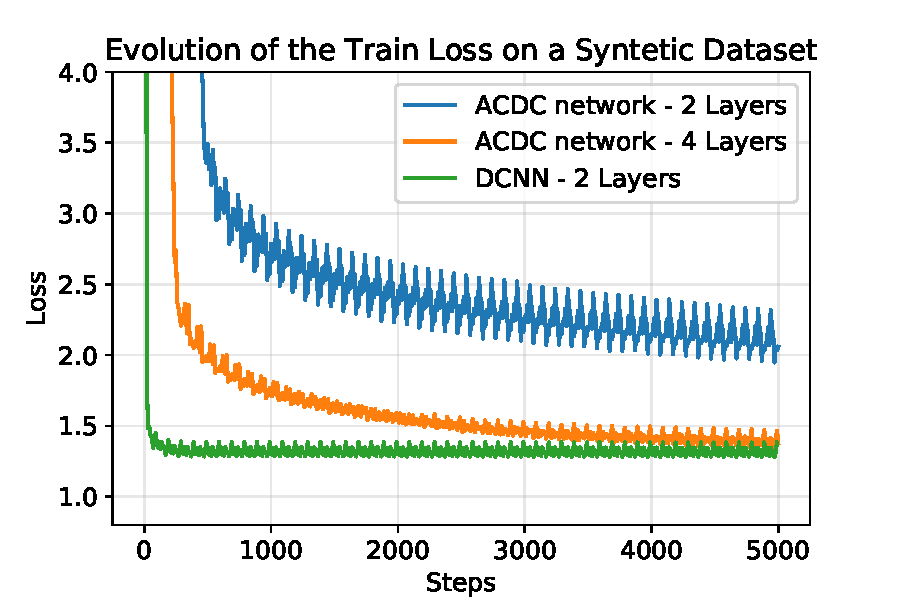
\includegraphics[scale=0.35]{figures/chapter3/acdc_regression.pdf}
%     \label{figure:adcd_regression}
%     }
% \subfigure[]{
%     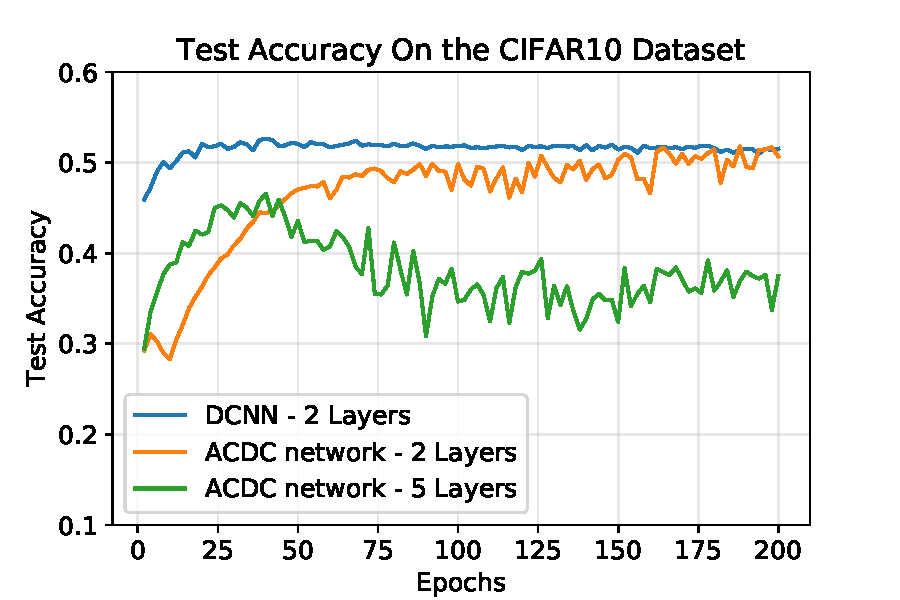
\includegraphics[scale=0.35]{figures/chapter3/acdc_cifar10.pdf}
%     \label{figure:acdc_cifar10}
%     }
% \caption{Comparison of DCNNs and \ACDC networks on two different tasks. Figure~\ref{figure:adcd_regression} shows the evolution of the training loss on a regression task with synthetic data. Figure~\ref{figure:acdc_cifar10} shows the test accuracy on the CIFAR-10 dataset.}
% \end{figure}



\begin{figure}
   \centering
   \begin{subfigure}[b]{0.49\textwidth}
       \centering
       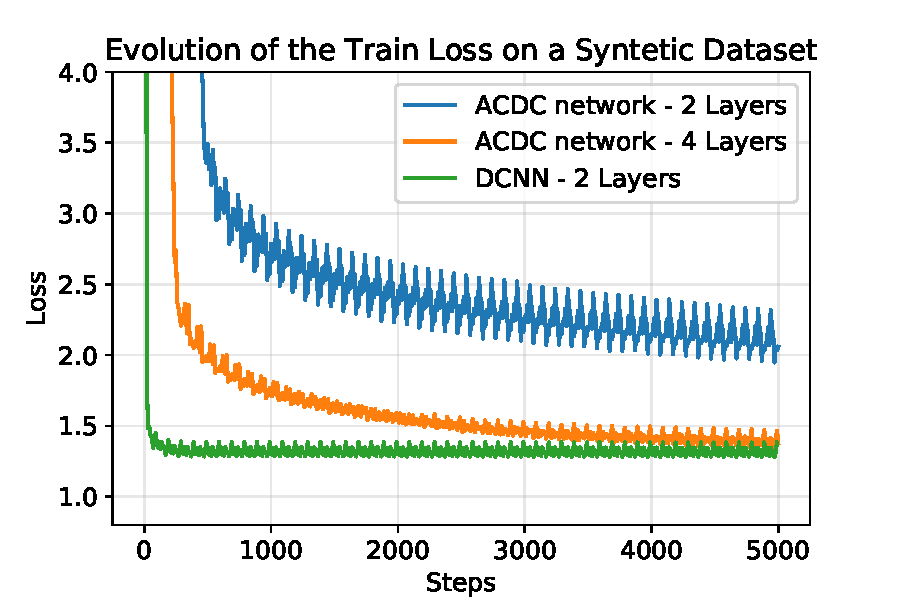
\includegraphics[width=\textwidth]{figures/chapter3/acdc_regression.pdf}
       \caption{Evolution of the training loss on a regression task with synthetic data.}
       \label{figure:acdc_regression}
   \end{subfigure}
   \hfill
   \begin{subfigure}[b]{0.49\textwidth}
       \centering
       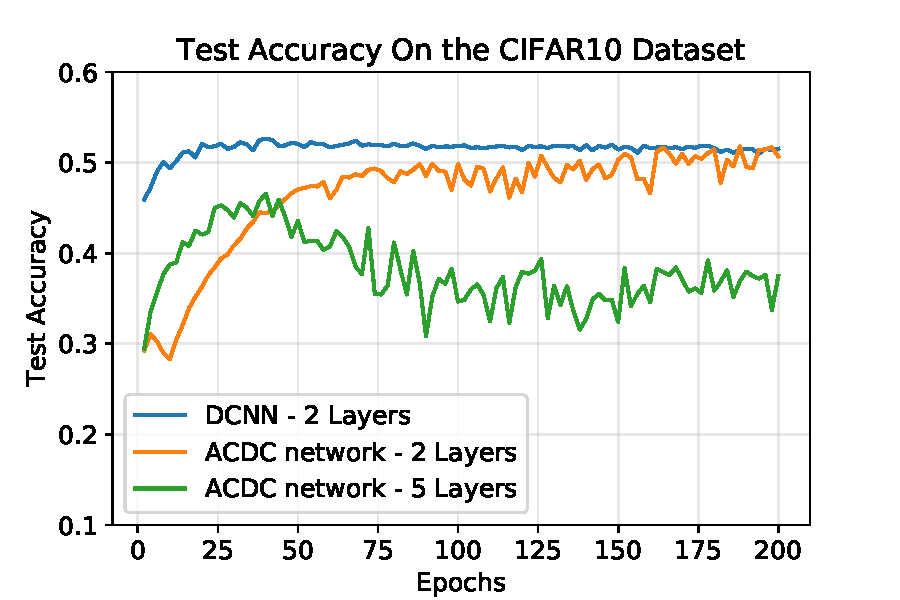
\includegraphics[width=\textwidth]{figures/chapter3/acdc_cifar10.pdf}
       \caption{Test accuracy on the CIFAR-10 dataset.~\\ \phantom{.}}
       \label{figure:acdc_cifar10}
   \end{subfigure}
   \caption{Comparison of DCNNs and \ACDC networks on two different tasks.}
\end{figure}




\paragraph{Comparison with \ACDC \citep{moczulski2015acdc}.}


In Section~\ref{section:ch3-related_work}, we have discussed the differences between the \ACDC framework and our approach from a theoretical perspective.
In this section, we conduct experiments to compare the performance of DCNNs with neural networks based on \ACDC layers. 
We first reproduce the experimental setting from \citet{moczulski2015acdc}, and compare both approaches using only linear networks (\ie networks without any ReLU activations).
The synthetic dataset has been created in order to reproduce the experiment on the regression linear problem proposed by~\citet{moczulski2015acdc}.
We draw $\Xmat$ and $\Wmat$ from a uniform distribution between [-1, +1] and $\epsilon$ from a normal distribution with mean 0 and variance $0.01$.
The relationship between $\Xmat$ and $\Ymat$ is define by $\Ymat = \Xmat\Wmat + \epsilon$. 
The results are presented in Figure~\ref{figure:acdc_regression}.
On this simple setting, while both architectures demonstrate good performance, we can observe that DCNNs offer a better convergence rate.
In Figure~\ref{figure:acdc_cifar10}, we compare neural networks with ReLU activations on CIFAR-10. 

We found that networks which are based only on \ACDC layers are difficult to train and offer poor accuracy on CIFAR-10 (we have tried different initialization schemes including the one from the original paper, and the one we introduce in this chapter).
\citet{moczulski2015acdc} manage to train a large VGG network  however these networks are generally highly redundant and the contribution of the structured layer is difficult to quantify. 
We also observe that adding a single dense layer improves the convergence rate of \ACDC in the linear case, which explains the good results of \citet{moczulski2015acdc}.
However, it is difficult to characterize the true contribution of the \ACDC layers when the network has a large number of expressive layers.

In contrast, deep DCNNs can be trained and offer good performance without additional dense layers (these results are in line with our experiments on the \yt dataset).
We can conclude that DCNNs are able to model complex relations at a low cost. 

% \begin{figure}[ht]
% \centering
% \subfigure[]{
%     \centering
%     
\includegraphics{graphs/cifar10_type.jpg}
%     \label{figure:cifar10_type}
%     }
% \subfigure[]{
%     \centering
%     
\includegraphics{graphs/scatterplot.jpg}
%     \label{figure:cifar10_with_channels_xp}
%     }
%     \caption{Figure~\ref{figure:cifar10_type}: network size vs. accuracy compared on Dense networks, DCNNs (our approach), DTNNs (our approach), neural networks based on Toeplitz matrices and neural networks based on Low Rank-based matrices. DCNNs outperforms alternatives structured approaches. Figure~\ref{figure:cifar10_with_channels_xp} shows the accuracy of different structured architecture given the number of trainable parameters.}
% \end{figure}



% \begin{figure}
%    \centering
%    \begin{subfigure}[b]{0.49\textwidth}
%        \centering
%        % 
\includegraphics[width=\textwidth]{graphs/cifar10_type.jpg}
%        \begin{tikzpicture}[scale=0.5]
\begin{axis}[
    legend cell align={left},
    xlabel={\large \#weights (x1000) },
    ylabel={Test Accuracy},
    xmin=21, xmax=370,
    ymin=0.2, ymax=0.6,
    legend pos=south east,
    ymajorgrids=true,
    grid style=dashed,
	]
    \addplot[color=red, line width=0.25mm, dashed] table [y=accuracy, x=weights]{figures/chapter3/data/cifar10/type/dense.dat};
    \addplot[mark=triangle, color=blue, line width=0.4mm] table [y=accuracy, x=weights]{figures/chapter3/data/cifar10/type/circulant.dat};
    \addplot[mark=square, color=red, line width=0.4mm] table [y=accuracy, x=weights]{figures/chapter3/data/cifar10/type/diag_toeplitz.dat};
    \addplot[mark=o, color=gray, line width=0.4mm] table [y=accuracy, x=weights]{figures/chapter3/data/cifar10/type/toeplitz.dat};
    \addplot[mark=diamond, color=brown, line width=0.4mm] table [y=accuracy, x=weights]{figures/chapter3/data/cifar10/type/low_rank.dat};
    \legend{
      Dense (9M weights),
      DCNN,
      DTNN,
      Toeplitz network,
      Low Rank network, 
     }
\end{axis}
\end{tikzpicture}

%        \caption{Network size vs. Accuracy compared on Dense networks, DCNNs (our approach), DTNNs (our approach), neural networks based on Toeplitz matrices and neural networks based on Low Rank-based matrices. DCNNs outperforms alternatives structured approaches.}
%        \label{figure:cifar10_type}
%    \end{subfigure}
%    \hfill
%    \begin{subfigure}[b]{0.49\textwidth}
%        \centering
%        % 
\includegraphics[width=\textwidth]{graphs/scatterplot.jpg}
%        \begin{tikzpicture}[scale=0.5]
\begin{axis}[
    xlabel={\large \#weights (x1000) },
    ylabel={Test Accuracy},
    legend pos=outer north east,
    legend cell align={left},
    ymajorgrids=true,
    grid style=dashed,
    ]
    % \addplot[mark=oplus*,blue] coordinates {(15, 0.6178)}; % Random Conv + Dense
    % \addplot[mark=oplus*,red] coordinates {(90, 0.8438)}; % Conv + Dense
    \addplot[mark=triangle*,blue] coordinates {(140, 0.7017)}; % ldr-sd (rank=1)
    \addplot[mark=triangle*,red] coordinates {(420, 0.7286)}; % ldr-sd (rank=10)
    \addplot[mark=diamond*,blue] coordinates {(110, 0.7111)}; % toeplitz-like (rank=1)
    \addplot[mark=diamond*,red] coordinates {(388, 0.7205)}; % toeplitz-like (rank=10)
    \addplot[mark=square*,green] coordinates {(124, 0.757)}; % Scattering + 1 DC
    \addplot[mark=square*,blue] coordinates {(217, 0.7856)}; % Scattering + 3 DC
    \addplot[mark=square*,red] coordinates {(66, 0.7535)}; % Scattering Avg pooling + 3 DC
    \addplot[mark=square*,brown] coordinates {(191, 0.764)}; % Scattering by channel + 4 DC
    % \addplot[mark=square*,green] coordinates {(131, 0.704)}; % Conv 32 + Max Pooling + 5 DC
    \legend{
        % Random Conv + Dense,
        % Conv + Dense,
        Scattering + LDR-SD (r=1),
        Scattering + LDR-SD (r=10),
        Scattering + Toeplitz-like (r=1),
        Scattering + Toeplitz-like (r=10),
        Scattering + 1 DC,
        Scattering + 3 DC,
        Scattering Avg pooling + 3 DC,
        Scattering by channel + 4 DC,
        % Conv + Max Pooling + DC,
    }
\end{axis}
\end{tikzpicture}

		
%        \caption{Accuracy of different structured architecture given the number of trainable parameters.~\\~\\~\\~\\~\\}
%        \label{figure:cifar10_with_channels_xp}
%    \end{subfigure}
% \end{figure}


\begin{figure}
   \centering
   \begin{tikzpicture}[scale=0.5]
\begin{axis}[
    legend cell align={left},
    xlabel={\large \#weights (x1000) },
    ylabel={Test Accuracy},
    xmin=21, xmax=370,
    ymin=0.2, ymax=0.6,
    legend pos=south east,
    ymajorgrids=true,
    grid style=dashed,
	]
    \addplot[color=red, line width=0.25mm, dashed] table [y=accuracy, x=weights]{figures/chapter3/data/cifar10/type/dense.dat};
    \addplot[mark=triangle, color=blue, line width=0.4mm] table [y=accuracy, x=weights]{figures/chapter3/data/cifar10/type/circulant.dat};
    \addplot[mark=square, color=red, line width=0.4mm] table [y=accuracy, x=weights]{figures/chapter3/data/cifar10/type/diag_toeplitz.dat};
    \addplot[mark=o, color=gray, line width=0.4mm] table [y=accuracy, x=weights]{figures/chapter3/data/cifar10/type/toeplitz.dat};
    \addplot[mark=diamond, color=brown, line width=0.4mm] table [y=accuracy, x=weights]{figures/chapter3/data/cifar10/type/low_rank.dat};
    \legend{
      Dense (9M weights),
      DCNN,
      DTNN,
      Toeplitz network,
      Low Rank network, 
     }
\end{axis}
\end{tikzpicture}

   \caption{Network size vs. Accuracy compared on Dense networks, DCNNs (our approach), DTNNs (our approach), neural networks based on Toeplitz matrices and neural networks based on Low Rank-based matrices. DCNNs outperforms alternatives structured approaches.}
   \label{figure:cifar10_type}
\end{figure}

\begin{figure}
   \centering
   \begin{tikzpicture}[scale=0.5]
\begin{axis}[
    xlabel={\large \#weights (x1000) },
    ylabel={Test Accuracy},
    legend pos=outer north east,
    legend cell align={left},
    ymajorgrids=true,
    grid style=dashed,
    ]
    % \addplot[mark=oplus*,blue] coordinates {(15, 0.6178)}; % Random Conv + Dense
    % \addplot[mark=oplus*,red] coordinates {(90, 0.8438)}; % Conv + Dense
    \addplot[mark=triangle*,blue] coordinates {(140, 0.7017)}; % ldr-sd (rank=1)
    \addplot[mark=triangle*,red] coordinates {(420, 0.7286)}; % ldr-sd (rank=10)
    \addplot[mark=diamond*,blue] coordinates {(110, 0.7111)}; % toeplitz-like (rank=1)
    \addplot[mark=diamond*,red] coordinates {(388, 0.7205)}; % toeplitz-like (rank=10)
    \addplot[mark=square*,green] coordinates {(124, 0.757)}; % Scattering + 1 DC
    \addplot[mark=square*,blue] coordinates {(217, 0.7856)}; % Scattering + 3 DC
    \addplot[mark=square*,red] coordinates {(66, 0.7535)}; % Scattering Avg pooling + 3 DC
    \addplot[mark=square*,brown] coordinates {(191, 0.764)}; % Scattering by channel + 4 DC
    % \addplot[mark=square*,green] coordinates {(131, 0.704)}; % Conv 32 + Max Pooling + 5 DC
    \legend{
        % Random Conv + Dense,
        % Conv + Dense,
        Scattering + LDR-SD (r=1),
        Scattering + LDR-SD (r=10),
        Scattering + Toeplitz-like (r=1),
        Scattering + Toeplitz-like (r=10),
        Scattering + 1 DC,
        Scattering + 3 DC,
        Scattering Avg pooling + 3 DC,
        Scattering by channel + 4 DC,
        % Conv + Max Pooling + DC,
    }
\end{axis}
\end{tikzpicture}

		
   \caption{Accuracy of different structured architecture given the number of trainable parameters.}
   \label{figure:cifar10_with_channels_xp}
\end{figure}


\paragraph{Comparison with Dense networks, Toeplitz networks and Low Rank networks.}
We now compare DCNNs with other state-of-the-art structured networks by measuring the accuracy on a flattened version of the CIFAR-10 dataset.
Our baseline is a dense feed-forward network with a fixed number of weights (9 million weights).
We compare with DCNNs and with DTNNs (see below), Toeplitz networks, and Low-Rank networks~\cite{8099498}.
We first consider Toeplitz networks which are stacked Toeplitz matrices interleaved with ReLU activations since Toeplitz matrices are closely related to circulant matrices.
However, Toeplitz networks have a different structure than DCNNs (they do not include diagonal matrices), therefore, we also experiment using DTNNs, a variant of DCNNs where all the circulant matrices have been replaced by Toeplitz matrices.
Finally we conduct experiments using networks based on low-rank matrices as they are also closely related to our work.
For each approach, we report the accuracy of several networks with a varying depth ranging from 1 to 40 (DCNNs, Toeplitz networks) and from 1 to 30 (from DTNNs).
For low-rank networks, we used a fixed depth network and increased the rank of each matrix from 7 to 40.
We also tried to increase the depth of low rank matrices, but we found that deep low-rank networks are difficult to train so we do not report the results here.
We compare all the networks based on the number of weights from 21K (0.2\% of the dense network) to 370K weights (4\% of the dense network) and we report the results in Figure~\ref{figure:cifar10_type}. 
First we can see that the size of the networks correlates positively with their accuracy which demonstrate successful training in all cases.
We can also see that the DCNNs achieves the maximum accuracy of 56\% with 20 layers ($\sim$ 200K weights) which is as good as the dense networks with only 2\% of the number of weights.
Other approaches also offer good trade-off but they are not able to reach the accuracy of a dense network.


\begin{table}[htb]
  \centering
  \begin{tabular}{lcc}
    \toprule
    \textbf{Architectures} & \textbf{\#Params} & \textbf{Acc.}  \\
    \midrule
    \textit{Dense} & \textit{9.4M}	& \textit{0.562} \\
    \textbf{\textit{DCNN $(5\ layers)$}} & \textbf{49K}	& \textbf{0.543} \\
    \textbf{\textit{DCNN $(2\ layers)$}} & \textbf{21K} & \textbf{0.536} \\
    LDR--TD	$(r = 2)$	        & 64K	& 0.511 \\
    LDR--TD	$(r = 3)$	        & 70K	& 0.473 \\
    Toeplitz-like $(r=2)$	    & 46K	& 0.483 \\
    Toeplitz-like $(r =3)$	    & 52K    & 0.496 \\
    \bottomrule
    \end{tabular}
    \caption{LDR networks compared with DCNNs on a flattend version of CIFAR-10. DCNNs outperform all LDR configurations with fewer weights. Remark: the numbers may differ from the original experiments by~\citet{Thomas_NIPS2018_8119} because we use the original dataset instead of a monochrome version.}
    \label{table:xp_ldr}
\end{table}

\begin{table}[htb]
  \centering
  \begin{tabular}{lcc}
    \toprule
    \textbf{Architectures} & \textbf{\#Params} & \textbf{Acc.}  \\
    \midrule
    \textbf{DC $(1\ layers)$} & \textbf{124K} & \textbf{0.757} \\
    \textbf{DC $(3\ layers)$} & \textbf{217K} & \textbf{0.785} \\
    \textbf{Ensemble x5 DC $(3\ layers)$} &  \textbf{1.08M} & \textbf{0.811} \\
    LDR-SD $(r=1)$ & 140K & 0.701 \\
    LDR-SD $(r=10)$ & 420K & 0.728 \\
    Toeplitz-like $(r=1)$ & 110K & 0.711 \\
    Toeplitz-like $(r=10)$ & 388K & 0.720 \\
    \bottomrule
    \end{tabular}
    \caption{Two depths scattering on CIFAR-10 followed by LDR or DC layer. Networks with DC layers outperform all LDR configurations with fewer weights.}
    \label{table:xp_ldr_scattering}
\end{table}


\paragraph{Comparison with LDR networks~\cite{Thomas_NIPS2018_8119}.}
We now compare DCNNs with the LDR framework using the network configuration experimented in the original paper: a single LDR structured layer followed by a dense layer.
In the LDR framework, we can change the size of a network by adjusting the rank of the residual matrix, effectively capturing matrices with a structure that is close to a known structure but not exactly (in the LDR framework, Toeplitz matrices can be encoded with a residual matrix with rank=2, so a matrix that can be encoded with a residual of rank=3 can be seen as Toeplitz-like.).
The results are presented in Table~\ref{table:xp_ldr} and demonstrate that DCNNs outperforms all LDR networks both in terms in size and accuracy.

\paragraph{Exploiting image features.}
Dense layers and DCNNs are not designed to capture task-specific features such as the translation invariance inherently useful in image classification.
We can further improve the accuracy of such general purpose architectures on image classification without dramatically increasing the number of trained parameters by stacking them on top of fixed (ie non-trained) transforms such as the scattering transform \cite{mallat2010recursive}.
In this section we compare the accuracy of various structured networks, enhanced with the scattering transform, on an image classification task, and run comparative experiments on CIFAR-10. 

Our test architecture consists of 2 depth scattering on the RGB images followed by a batch norm and LDR or DC layer.
To vary the number of parameters of Scattering+LDR architecture, we increase the rank of the matrix (stacking several LDR matrices quickly exhausted the memory).
The Figure \ref{figure:cifar10_with_channels_xp} and \ref{table:xp_ldr_scattering} shows the accuracy of these architectures given the number of trainable parameters.

First, we can see that the DCNN architecture very much benefits from the scattering transform and is able to reach a competitive accuracy over 78\%.
We can also see that scattering followed by a DC layer systematically outperforms scattering + LDR or scattering + Toeplitz-like with less parameters. 


\subsection{Comparison with other compression based approaches}


\begin{table}
  \centering
    \caption{Comparison with compression based approaches}
    \begin{tabular}{lcrc}
    \toprule
    \multicolumn{1}{c}{\textbf{Architecture}} & \multicolumn{1}{c}{\textbf{\#Params}} & \textbf{Error (\%)} \\
    \hline \\
    \textit{LeNet \cite{Lecun98gradient-basedlearning}} & \textit{4 257 674} & \textit{0.61} \\
    \multirow{2}[0]{*}{\textbf{DCNN}} & \textbf{25 620} & \textbf{1.74} \\
          & \textbf{31 764} & \textbf{1.60} \\
    \multirow{2}[0]{*}{HashNet \cite{Chen_Hashing_Trick}} & 46 875 & 2.79 \\
          &  78 125 & 1.99 \\
    \multirow{2}[0]{*}{Dark Knowledge \cite{44873}} & 46 875 & 6.32 \\
          &  78 125 & 2.16 \\
    \bottomrule
    \end{tabular}%
  \label{tab:mnist}%
\end{table}%


We provide a comparison with other compression based approaches such as HashNet \cite{Chen_Hashing_Trick}, Dark Knowledge \cite{44873} and Fast Food Transform (FF) \cite{7410530}. 
Table~\ref{tab:mnist} shows the test error of DCNN against other know compression techniques on the MNIST datasets. We can observe that DCNN outperform easily HashNet \cite{Chen_Hashing_Trick} and Dark Knowledge \cite{44873} with fewer number of parameters. The architecture with Fast Food (FF) \cite{7410530} achieves better performance but with convolutional layers and only $1$ Fast Food Layer as the last Softmax layer. 


\subsection{Large-scale video classification on the \yt dataset}

To understand the performance of deep DCNNs on large scale applications, we conducted experiments on the \yt video classification with 3.8 training examples introduced by~\citet{abu2016youtube}.
Notice that we favour this experiment over ImageNet applications because modern image classification architectures involve a large number of convolutional layers, and compressing convolutional layers is out of our scope. 
Also, as mentioned earlier, testing the performance of DCNN architectures mixed with a large number of expressive layers makes little sense.
The \yt includes two datasets describing 8 million labeled videos.
Both datasets contain audio and video features for each video.
In the first dataset (\emph{aggregated}) all audio and video features have been aggregated every 300 frames.
The second dataset (\emph{full}) contains the descriptors for all the frames.
To compare the models we use the GAP metric (Global Average Precision) proposed by~\citet{abu2016youtube}.
On the simpler \emph{aggregated} dataset we compared off-the-shelf DCNNs with a dense baseline with 5.7M weights.
On the full dataset, we designed three new compact architectures based on the state-of-the-art architecture introduced by~\citet{abu2016youtube}. 

\paragraph{Experiments on the aggregated dataset with DCNNs:}
We compared DCNNs with a dense baseline with 5.7 millions weights.
The goal of this experiment is to discover a good trade-off between depth and model accuracy.
To compare the models we use the GAP metric (Global Average Precision) following the experimental protocol in~\cite{abu2016youtube}, to compare our experiments. 

Table~\ref{table:youtube_agg_xp} shows the results of our experiments on the {\em aggrgated} \yt dataset in terms of number of weights, compression rate and GAP.
We can see that the compression ratio offered by the circulant architectures is high.
This comes at the cost of a little decrease of GAP measure.
The 32 layers DCNN is 46 times smaller than the original model in terms of number of parameters while having a close performance. 


\begin{table}
  \centering
  \caption{This table shows the GAP score for the \yt dataset with DCNNs. We can see a large increase in the score with deeper networks.}
  \begin{tabular}{lccc}
    \toprule
    \textbf{Architecture} & \textbf{\#Weights} &
    \textbf{GAP@20} \\
    \hline \\
    \textit{original} & \textit{5.7M} & \textit{0.773} \\
    4 DC & 25 410  (\textit{\textbf{0.44}}) & 0.599   \\
    32 DC  & 122 178 \textit{(2.11)} & 0.685   \\
    4 DC + 1 FC & 4.46M \textit{(77)} & \textbf{0.747} \\
  \hline
  \end{tabular}
  \label{table:youtube_agg_xp}
\end{table}

\begin{table}
  \centering
  \caption{This table shows the GAP score for the \yt dataset with different layer represented with our DC decomposition.}
  \begin{tabular}{lccc}
  \toprule
  \textbf{Architecture} & \textbf{\#Weights} & \textbf{GAP@20} \\
  \hline \\
  \textit{original} & \textit{45M} & \textit{0.846} \\
  DBoF with DC   & 36M (\textit{80}) & 0.838 \\
  FC with DC    & 41M (\textit{91}) & \textbf{0.845} \\
  MoE with DC   & 12M (\textit{\textbf{26}}) & 0.805 \\
  \hline
  \end{tabular}
  \label{table:youtube_full_xp}
\end{table}

\paragraph{Experiments with DCNNs Deep Bag-of-Frames Architecture:}
The Deep Bag-of-Frames architecture can be decomposed into three blocks of layers, as illustrated in Figure~\ref{figure:archi_youtube}.
The first block of layers, composed of the Deep Bag-of-Frames embedding (DBoF), is meant to model an embedding of these frames in order to make a simple representation of each video.
A second block of fully connected layers (FC) reduces the dimensionality of the output of the embedding and merges the resulting output with a concatenation operation.
Finally, the classification block uses a combination of Mixtures-of-Experts (MoE)~\cite{716791,45619} and Context Gating~\cite{miech2017learnable} to calculate the final class probabilities.
Table~\ref{table:youtube_full_xp} shows the results in terms of number of weights, size of the model (MB) and GAP on the full dataset, replacing the DBoF block reduces the size of the network without impacting the accuracy.
We obtain the best compression ratio by replacing the MoE block with DCNNs (26\%) of the size of the original dataset with a GAP score of 0.805 (95\% of the score obtained with the original architecture).
We conclude that DCNN are both theoretically sound and of practical interest in real, large scale applications.

\begin{figure}[htb]
  \centering
  \tikzset{%
  >={Latex[width=2mm,length=2mm]},
  % Specifications for style of nodes:
            base/.style = {rectangle, draw=black, text centered, font=\sffamily},
             box/.style = {base, rounded corners, text depth=3cm, minimum height=4cm, minimum width=3cm},
     transparent/.style = {rectangle, draw=black},
       circulant/.style = {base, fill=yellow!30},
       embedding/.style = {base, fill=blue!30, minimum width=2.5cm, minimum height=1cm},
           other/.style = {base, fill=white!30,  minimum width=2cm, minimum height=1cm},
              fc/.style = {base, fill=orange!30, minimum width=1.5cm, minimum height=1cm},
          gating/.style = {base, fill=green!30, minimum width=2cm, text width=2cm, minimum height=1cm},
             moe/.style = {base, fill=purple!30, minimum width=1.5cm, minimum height=1cm},
}

\begin{tikzpicture}[every node/.style={fill=white, font=\sffamily}, align=center]

  \draw (0.0, +2.)  node [other, draw=none] {\textbf{Embedding}};
  \draw (+3.7, +2.)  node [other, draw=none] {\textbf{Dim Reduction}};
  \draw (+8.0, +2.)  node [other, draw=none] {\textbf{Classification}};

  \draw (0, +0.8)  node [embedding] {Video};
  \draw (0, -0.8)  node [embedding] {Audio};

  \draw (+2.5, +0.8)  node (fc) [fc] {FC};
  \draw (+2.5, -0.8)  node (fc) [fc] {FC};

  \draw (+4.75, 0)  node (fc) [other] {concat};
  \draw (+7.0, 0)  node (moe) [moe] {MoE};
  \draw (+9.25, 0)  node (gating2) [gating] {Context Gating};
 
  \draw (+1.5, +2) [dashed] -- (+1.5, -1.7);
  \draw (+6, +2) [dashed] -- (+6, -1.7);
  
\end{tikzpicture}

  \caption{This figure shows the state-of-the-art neural network architecture, initially proposed by~\citet{abu2016youtube} and later improved by~\citet{miech2017learnable}, used in our experiment.}
  \label{figure:archi_youtube}
\end{figure}

\paragraph{Architectures \& Hyper-Parameters:} 
For the first set of our experiments (\emph{experiments on CIFAR-10}), we train all networks for 200 epochs, a batch size of 200, Leaky ReLU activation with a different slope.
We minimize the Cross Entropy Loss with Adam optimizer and use a piecewise constant learning rate of $5 \times 10^{-5}$, $2.5\times10^{-5}$, $5\times10^{-6}$ and $1\times10^{-6}$ after respectively 40K, 60K and 80K steps.
For the \yt dataset experiments, we built a neural network based on the SOTA architecture initially proposed by~\citet{abu2016youtube} and later improved by~\citet{miech2017learnable}.
Remark that no convolution layer is involved in this application since the input vectors are embeddings of video frames processed using state-of-the-art convolutional neural networks trained on ImageNet.
We trained our models with the CrossEntropy loss and used Adam optimizer with a 0.0002 learning rate and a 0.8 exponential decay every 4 million examples.
All fully connected layers are composed of 512 units.
DBoF, NetVLAD and NetFV are respectively 8192, 64 and 64 of cluster size for video frames and 4096, 32, 32 for audio frames.
We used 4 mixtures for the MoE Layer.
We used all the available 300 frames for the DBoF embedding.
In order to stabilize and accelerate the training, we used batch normalization before each non linear activation and gradient clipping. 

%%%%%%%%%%%%%%%%%%%%%%%%%%%%%%%%%%%%%%%%%%%%%%%%%%%%%%%%%%%%%%%%%%%%%%%%%%%%%%%
\section{Conclusion}
\label{section:ch3-conclusion}
%%%%%%%%%%%%%%%%%%%%%%%%%%%%%%%%%%%%%%%%%%%%%%%%%%%%%%%%%%%%%%%%%%%%%%%%%%%%%%%

This chapter deals with the training of diagonal circulant neural networks.
To the best of our knowledge, training such networks with a large number of layers had not been done before.
We also endowed this kind of models with theoretical guarantees, hence enriching and refining previous theoretical work from the literature.
More importantly, we showed that DCNNs outperform their competing structured alternatives, including the very recent general approach based on LDR networks.
Our results suggest that stacking diagonal circulant layers with non linearities improves the convergence rate and the final accuracy of the network.
Formally proving these statements constitutes the future directions of this work.
We would like to generalize the good results of DCNNs to convolutional neural networks.
We also believe that circulant matrices deserve a particular attention in deep learning because of their strong ties with convolutions: a circulant matrix operator is equivalent to the convolution operator with circular paddings.
This fact makes any contribution to the area of circulant matrices particularly relevant to the field of deep learning with impacts beyond the problem of designing compact models.
As future work, we would like to generalize our results to deep convolutional neural networks. 


% \section{Notations \& Definition}
% We note $\mathfrak{R}(z)$ and $\mathfrak{I}(z)$  the real and imaginary parts the complex number $z$.
% We note $\left(\ \cdot\ \right)_{t}$ is the $t^{th}$ component of a vector.
% Let $\ci$ be the imaginary number defined by $\ci^2=-1$.
% Define $\mathbf{1}_{n}$ as the \emph{n-}vector of ones.
% The rectified linear unit on the complex domain is defined by $\relu(z)=\max\left(0,\mathfrak{R}(z)\right)+\ci\max\left(0,\mathfrak{I}(z)\right)$.
% In the rest of this paper, we call $L$ and $n$ respectively the depth and the width of the network.
% Moreover, we call {\em total rank $k$}, the sum of the ranks of the matrices $W_{1}\ldots W_{L}$. ie $k = \sum_{i=1}^L rank(W_i)$.
% The notation $\left|\ \cdot\ \right|$ refers to the complex modulus.
% We introduce some necessary definitions regarding neural networks.  

% \begin{definition}[Deep ReLU network]\label{def:deep_relu_network-appendix}
% Given $L$ weight matrices $W = (W_1, \ldots, W_L)$ with $W_i \in \mathbb C^{n\times n}$ and  $L$ bias vectors $b = (b_1, \ldots, b_L)$  with  $b_i \in \mathbb C^n$, a {\em deep $\relu$ network} is a function $f_{W_L, b_L} : \mathbb C^n \rightarrow \mathbb C^n$ such that $f_{W, b}(x) =  (f_{W_L, b_L} \circ \ldots \circ f_{W_1, b_1})(x)$ where $f_{W_i, b_i}(x) = \phi(W_i x + b_i)$ and $\phi(.)$ is a $\relu$ non-linearity
% \footnote{Because our networks deal with complex numbers, we use an extension of the $\relu$ function to the complex domain. The most straightforward extension defined in \cite{DBLP:conf/iclr/TrabelsiBZSSSMR18} is as follows: $\mathrm{\relu}(z) = \relu \left( \mathfrak{R}(z) \right) +i \relu \left(\mathfrak{I}(z)\right)$, where $\mathfrak{R}$ and $\mathfrak{I}$ refer to the real and imaginary parts of $z$.}
% In the rest of this paper, we call $L$ and $n$ respectively the depth and the width of the network. Moreover, we call {\em total rank $k$}, the sum of the ranks of the matrices $W_{1}\ldots W_{L}$. ie $k = \sum_{i=1}^L rank(W_i)$.
% \end{definition}




% \section{Proofs of Section 3}

% \begin{theorem}
% (Reformulation from Huhtanen et al. \cite{Huhtanen2015})\label{theorem:huhtanen-appendix}
% For any given matrix $A\in\mathbb{C}^{n\times n}$, for any $\epsilon > 0$, there exists a sequence of matrices $B_1 \ldots B_{2n-1}$ where $B_{i}$ is a circulant matrix if $i$ is odd, and a diagonal matrix otherwise, such that $\norm{ B_{1}B_{2}\ldots B_{2n-1}-A } < \epsilon$.
% Moreover, if $A$ can be decomposed as $A=\sum_{i=1}^{k}D_{i}S^{i-1}$ where $S$ is the cyclic-shift matrix and $D_{1}\ldots D_{k}$ are diagonal matrices, then $A$ can be written as a product $B_{1}B_{2}\ldots B_{2k-1}$ where $B_{i}$ is a circulant matrix if $i$ is odd, and a diagonal matrix otherwise.
% \end{theorem}
%


% \begin{theorem}(Rank-based circulant decomposition) \label{theorem:rank-decomposition-appendix}
% Let $A\in\mathbb{C}^{n\times n}$ be a matrix of rank at most $k$. Assume that $n$ can be divided by $k$. For
% any $\epsilon>0$, there exists a sequence of $4k+1$ matrices $B_{1},\ldots,B_{4k+1},$ where $B_{i}$ is a circulant matrix if $i$ is odd, and a diagonal matrix otherwise, such that $\Vert B_1B_2\ldots B_{4k+1} - A\Vert < \epsilon$
% \end{theorem}

% \section{Proofs of Section 4}
%
% \begin{lemma} \label{lemma:product_of_mat_to_DNN}
% Let $W_{L},\ldots W_{1}\in\mathbb{C}^{n\times n}$, $b\in\mathbb{C}^{n}$ and let $\mathcal{X}\subset\mathbb{C}^{n}$ be a bounded set.
% There exists $\beta_{L} \ldots \beta_{1} \in \mathbb{C}^{n}$ such that for all $x \in \mathcal{X}$ we have $f_{W_{L},\beta_{L}} \circ \ldots \circ f_{W_{1},\beta_{1}}(x) = \relu \left(W_{L}W_{L-1} \ldots W_{1}x+b \right)$.
% \end{lemma}
%
% \begin{proof}[\proofreflem{lemma:product_of_mat_to_DNN}]
% Define $S = \left\{ \left(\left(\prod_{k=1}^{j} \Wmat_{k} \right) \xvec \right)_{t}: \xvec \in \mathcal{X}, t \in [n], j \in [L] \right\}$.
% Let $\Omega = \max\left\{ \mathfrak{R}(v): v \in S \right\} + \ci \max\left\{ \mathfrak{I}(v):v \in S \right\}$.
% Intuitively, the real and imaginary parts of $\Omega$ are the largest any activation in the network can have.
% Define $h_{j}(\xvec) = \Wmat_{j}\xvec + \beta_{j}$. Let $\beta_{1} = \Omega \mathbf{1}_{n}$.
% Clearly, for all $\xvec \in \mathcal{X}$ we have $h_{1}(\xvec)\ge0$, so $\relu \circ h_{1}(\xvec) = h_{1}(\xvec)$.
% More generally, for all $j < n-1$ define $\beta_{j+1} = \mathbf{1}_{n} \Omega - \Wmat_{j+1} \beta_{j}$.
% It is easy to see that for all $j < n$ we have $h_{j} \circ \ldots \circ h_{1}(\xvec) = \Wmat_{j}\Wmat_{j-1} \ldots \Wmat_{1}x + \mathbf{1}_{n} \Omega$.
% This guarantees that for all $j < n$, $h_{j} \circ \ldots \circ h_{1}(\xvec) = \relu \circ h_{j} \circ \ldots \circ \relu \circ h_{1}(\xvec)$.
% Finally, define $\beta_{L} = b - A_{L} \beta_{L-1}$.
% We have, $\relu \circ h_{L} \circ \ldots \circ \relu \circ h_{1}(\xvec) = \relu \left(\Wmat_{j} \ldots \Wmat_{1} \xvec + b \right)$. 
% \end{proof}
%
% \begin{lemma}\label{mainth_-appendix}
% Let $\mathcal{N}$ be a deep ReLU network of width $n$ and depth $L$, and let $\mathcal{X} \subset \mathbb{C}^{n}$ be a bounded set. For any $\epsilon > 0$, there exists a DCNN $\mathcal{N}'$ of width $n$ and of depth $(2n-1)L$ such that $\Vert \mathcal{N}(x) - \mathcal{N}'(x) \Vert < \epsilon$ for all $x \in \mathcal{X}$.
% \end{lemma}
%

% \begin{corollary} \label{cor:universal-appendix}
% Bounded width DCNNs are universal approximators in the following sense: for any continuous function $f:[0,1]^{n}\rightarrow\mathbb{R}_+$ of bounded supremum norm,
% for any $\epsilon>0$, there exists a DCNN
% $\mathcal{N}_{\epsilon}$ of width $n+3$ such that $\forall x\in[0,1]^{n+3}$, $\left|f(x_{1}\ldots x_{n})-\left(\mathcal{N}_{\epsilon}\left(x\right)\right)_{1}\right|<\epsilon$, where $\left(\cdot\right)_{i}$ represents the $i^{th}$ component of a vector.
% \end{corollary}

% \begin{theorem}[Rank-based expressive power of diagonal circulant neural networks] \label{theorem:low_rank_nn-appendix}
% Let $\mathcal{N}:f_{W_{L},b_{L}} \circ \ldots \circ f_{W_{1},b_{1}}$ be a deep ReLU network of width $n$, depth $L$ and a total rank $k$.
% Assume $n$ is a power of $2$.
% Let $\mathcal{X} \subset \mathbb{C}^{n}$ be a bounded set.
% For any $\epsilon>0$, there exists a DCNN $\mathcal{N}'$ of width $n$ such that $\norm{ \mathcal{N}(x)-\mathcal{N}'(x)} <\epsilon$ for all $x\in\mathcal{X}$.
% In addition, the depth of $\mathcal{N}'$ is bounded by $9k$.
% Moreover, if the rank of each matrix $A_i$ divides $n$, then the depth of $\mathcal{N}'$ is bounded by $L+4k$.
% \end{theorem}
%
% \begin{proof} \emph{(Theorem \ref{theorem:low_rank_nn-appendix})}
% Let $k_{1} \ldots k_{L}$ be the ranks of matrices $\Wmat_{1} \ldots \Wmat_{L}$, which are $n$-by-$n$ matrices.
% For all $i$, there exists $k_{i}' \in \{k_{i} \ldots 2k_{i}\}$ such that $k'_{i}$ is a power of $2$.
% Due to the fact that $n$ is also a power of $2$, $k'_{i}$ divides $n$.
% By Theorem~\ref{theorem:rank-decomposition-appendix}, for all $i$ each matrix $\Wmat_{i}$ can be decomposed as an alternating product of diagonal-circulant matrices $\Bmat_{i,1} \ldots \Bmat_{i,4k'_{i}+1}$ such that $\norm{ \Wmat_{i} - \Bmat_{i,1} \times \ldots \times \Bmat_{i,4k'_{i}+1}} < \epsilon$.
% Using the exact same technique as in Lemma~\ref{lemma:dcnn_approx_neural_network}, we can build a DCNN $\mathcal{N}'$ using matrices $\Bmat_{1,1} \ldots \Bmat_{L,4k'_{L}+1}$, such that $\norm{ \mathcal{N}(\xvec) - \mathcal{N}'(\xvec)} < \epsilon$ for all $\xvec \in \mathcal{X}$.
% The total number of layers is $\sum_{i}\left(4k_{i}'+1\right)\le L+8\sum_{i}k_{i}\le L+8.
% \textrm{total rank} \le 9.\textrm{total rank}$.
% \end{proof}
%
% Finally, what if we choose to use small depth networks to approximate deep ReLU networks where matrices are not of low rank?
% To answer this question, we first need to show the negative impact of replacing matrices by their low rank approximators in neural networks:
%
% \begin{proposition} \label{proposition:relu_to_svd}
% Let $\mathcal{N} = f_{W_{L},b_{L}} \circ \ldots \circ f_{W_{1},b_{1}}$ be a Deep ReLU network, where $W_{i} \in \mathbb{C}^{n \times n}, b_{i} \in \mathbb{C}^{n}$ for all $i \in [L]$. Let $\tilde{W}_{i}$ be the matrix obtained by an SVD approximation of rank $k$ of matrix $W_{i}$. Let $\sigma_{i,j}$ be the $j^{th}$ singular value of $W_{i}$. Define $\tilde{\mathcal{N}} = f_{\tilde{W_{L}},b_{L}} \circ \ldots \circ f_{\tilde{W_{1}},b_{1}}$. Then, for any $x \in \mathbb{C}^{n}$, we have:
% \begin{equation}
% \norm{ \mathcal{N}\left(x\right) - \tilde{\mathcal{N}} \left(x\right)} \le \frac{\left(\sigma_{max,1}^{L}-1\right)R\sigma_{max,k}}{\sigma_{max,1}-1}
% \end{equation}
% where $R$ is an upper bound on norm of the output of any layer in $\mathcal{N}$, and $\sigma_{max,j}=\max_{i}\sigma_{i,j}$.
% \end{proposition}
%
% \begin{proof} \emph{(Proposition~\ref{proposition:relu_to_svd})}
% Let $x_{0} \in \mathbb{C}^{n}$ and $\tilde{x}_{0} = x_{0}$.
% For all $i \in [L]$, define $x_{i} = \relu \left(W_{i} x_{i-1} + b \right)$ and $\tilde{x}_{i} = \relu \left( \tilde{W_{i}} \tilde{x}_{i-1} + b \right)$.
% By lemma \ref{lemma:bound_one_layer}, we have 
% \begin{equation}
%   \norm{ x_{i}-\tilde{x}_{i}} \le\sigma_{i,k+1}\norm{ x_{i-1}} +\sigma_{i,1}\norm{ x_{i-1}-\tilde{x}_{i-1}} 
% \end{equation}
% Observe that for any sequence $a_{0},a_{1}\ldots$ defined recurrently by $a_{0}=0$ and $a_{i}=ra_{i-1}+s$, the recurrence relation can be unfold as follows: $a_{i}=\frac{s\left(r^{i}-1\right)}{r-1}$.
% We can apply this formula to bound our error as follows:
% \begin{equation}
%   \norm{ x_{l} - \tilde{x}_{l} } \le\frac{ \left( \sigma_{max,1}^{l} - 1 \right) \sigma_{max,k} \max_{i} \norm{ x_{i} } }{\sigma_{max,1}-1}
% \end{equation}
% \end{proof}
%
% \begin{lemma} \label{lemma:bound_one_layer}
% Let $W\in\mathbb{C}^{n\times n}$ with singular values $\sigma_{1}\ldots\sigma_{n}$, and let $x,\tilde{x}\in\mathbb{C}^{n}$.
% Let $\tilde{W}$ be the matrix obtained by a SVD approximation of rank $k$ of matrix $W$.
% Then we have:
% \begin{equation}
%   \norm{ \relu \left( Wx + b \right) - \relu \left( \tilde{W}\tilde{x}+b\right)} \le\sigma_{k+1}\norm{ x} +\sigma_{1}\norm{ \tilde{x}-x} 
% \end{equation}
% \end{lemma}
%
% \begin{proof} {\em (Lemma~\ref{lemma:bound_one_layer})}
% Recall that $\norm{ W} _{2}=\sup_{z}\frac{\norm{ Wz}_2 }{\norm{ z}_2 }=\sigma_{1}=\norm{ \tilde{W}} _{2}$, because $\sigma_{1}$ is the greatest singular value of both $W$ and $\tilde{W}$. Also, note that $\norm{ W-\tilde{W}} _{2}=\sigma_{k+1}$. Let us bound the formula without ReLUs:
%
% \begin{align*}
%   \norm{ \left(Wx+b\right)-\left(\tilde{W}\tilde{x}+b\right)}  & =\norm{ \left(Wx+b\right)-\left(\tilde{W}\tilde{x}+b\right)} \\
%    & =\norm{ Wx-\tilde{W}x-\tilde{W}\left(\tilde{x}-x\right)} \\
%    & \le \norm{ \left(W-\tilde{W}\right)x} +\norm{ \tilde{W}} _{2}\norm{ \tilde{x}-x} \\
%    & \le \norm{ x} \sigma_{k+1}+\sigma_{1}\norm{ \tilde{x}-x} 
% \end{align*}
%
% Finally, it is easy to see that for any pair of vectors $\avec,\bvec \in \Cn$, we have $\norm{ \relu(\avec) - \relu(\bvec)} \le \norm{\avec - \bvec} $.
% This concludes the proof.
% \end{proof}
%
% \begin{corollary} \label{corollary:relu_to_circ}
% Consider any deep ReLU network $\mathcal{N} = f_{W_{L},b_{L}} \circ \ldots \circ f_{W_{1},b_{1}}$ of depth $L$ and width $n$.
% Let $\sigma_{max,j} = \max_{i} \sigma_{i,j}$ where $\sigma_{i,j}$ is the $j^{th}$ singular value of $W_{i}$.
% Let $\mathcal{X} \subset \mathbb{C}^{n}$ be a bounded set.
% Let $k$ be an integer dividing $n$.
% There exists a DCNN $\mathcal{N}' = f_{D_{m}C_{m},b'_{m}} \circ \ldots \circ f_{D_{1}C_{1},b'_{1}}$ of width $n$ and of depth $m=L(4k+1)$, such that for any $x\in\mathcal{X}$:
% \begin{equation}
%   \norm{ \mathcal{N}\left(x\right) - \mathcal{N}'\left(x\right)} < \frac{\left(\sigma_{max,1}^{L}-1\right)R\sigma_{max,k}}{\sigma_{max,1}-1}
% \end{equation}
% where $R$ is an upper bound on the norm of the outputs of each layer in $\mathcal{N}$.
% \end{corollary}
%
% \begin{proof} \emph{(Corollary \ref{corollary:relu_to_circ})}
% Let $\tilde{\mathcal{N}}=f_{\tilde{W_{L}},b_{L}}\circ\ldots\circ f_{\tilde{W_{1}},b_{1}}$, where each $\tilde{W}_{i}$ is the matrix obtained by an SVD approximation of rank $k$ of matrix $W_{i}$.
% With Proposition~\ref{proposition:relu_to_svd}, we have an error bound on $\Vert \mathcal{N}\left(x\right)-\tilde{\mathcal{N}}\left(x\right)\Vert $.
% Now each matrix $\tilde{W}_{i}$ can be replaced by a product of $k$ diagonal-circulant matrices.
% By theorem \ref{theorem:low_rank_nn-appendix}, this product yields a DCNN of depth $m = L(4k+1)$, strictly equivalent to $\tilde{\mathcal{N}}$ on $\mathcal{X}$.
% This conludes the proof.
% \end{proof}
%



  
%%%%%%%%%%%%%%%%%%%%%%%%%%%%%%%%%%%%%%%%%%%%%%%%%%%%%%%%%%%%%%%%%%%%%%%%%%%%%%%
\chapter{Lipschitz Bound of Convolutional Neural Network}
\label{chapter:lipschitz_bound}
%%%%%%%%%%%%%%%%%%%%%%%%%%%%%%%%%%%%%%%%%%%%%%%%%%%%%%%%%%%%%%%%%%%%%%%%%%%%%%%
\localtableofcontents

% \begin{abstract}
% This paper tackles the problem of Lipschitz regularization of Convolutional Neural Networks. Lipschitz regularity is now established as a key property of modern deep learning with implications in training stability, generalization, robustness against adversarial examples, etc. However, computing the exact value of the Lipschitz constant of a neural network is known to be NP-hard. Recent attempts from the literature introduce upper bounds to approximate this constant that are either efficient but loose or accurate but computationally expensive. In this work, by leveraging the theory of Toeplitz matrices, we introduce a new upper bound for convolutional layers that is both tight and easy to compute. Based on this result we devise an algorithm to train Lipschitz regularized Convolutional Neural Networks.
% \end{abstract}


%%%%%%%%%%%%%%%%%%%%%%%%%%%%%%%%%%%%%%%%%%%%%%%%%%%%%%%%%%%%%%%%%%%%%%%%%%%%%%%
\section{Introduction}
\label{section:ch4-introduction}
%%%%%%%%%%%%%%%%%%%%%%%%%%%%%%%%%%%%%%%%%%%%%%%%%%%%%%%%%%%%%%%%%%%%%%%%%%%%%%%


The last few years have witnessed a growing interest in Lipschitz regularization of neural networks, with the aim of improving their generalization~\cite{bartlett2017spectrally}, their robustness to adversarial attacks~\cite{tsuzuku2018lipschitz, farnia2018generalizable}, or their generation abilities (\eg for GANs: \cite{miyato2018spectral,arjovsky2017wasserstein}).
Unfortunately computing  the exact Lipschitz constant of a neural network is NP-hard~\cite{scaman2018lipschitz} and in practice, existing techniques such as~\cite{scaman2018lipschitz, NIPS2019_9319} or~\cite{latorre2020lipschitz} are difficult to implement for neural networks with more than one or two layers, which hinders their use in deep learning applications.

To overcome this difficulty, most of the work has focused on computing the Lipschitz constant of {\em individual layers} instead.
The product of the Lipschitz constant of each layer is an upper-bound for the Lipschitz constant of the entire network, and it can be used as a surrogate to perform Lipschitz regularization.
Since most common activation functions (such as ReLU) have a Lipschitz constant equal to one, the main bottleneck is to compute the Lipschitz constant of the underlying linear application which is equal to its maximal singular value.
The work in this line of research mainly relies on the celebrated iterative algorithm by~\citet{golub2000eigenvalue} used to approximate the maximum singular value of a linear function.
Although generic and accurate, this technique is also computationally expensive, which impedes its usage in large training settings. 

In this paper we introduce a new tight and easy to compute  upper bound on the largest singular value of convolution layers.
We rely on Toeplitz matrix theory and its links with Fourier analysis.
It is known that the sequence of elements that characterizes a Toeplitz matrix is the Fourier transform of a given trigonometric polynomial.
We extend this result to doubly-block Toeplitz matrices (\ie block Toeplitz matrices where each block is Toeplitz) and devise a bound on the singular values of these matrices as a function of a multivariate trigonometric polynomial.
Implementing this bound in the context of convolutional neural networks, requires further to consider a sequence of doubly-block Toeplitz matrices, since the entries are commonly chosen to be tensors of more than one dimension.
As a main result, we devise an upper bound for a stacked sequence of doubly-block Toeplitz matrices, which fits well the requirements of CNNs, both in terms of applicability and efficiency.
From our analysis immediately follows an algorithm for bounding the Lipschitz constant of a convolutional layer, and by extension the Lipschitz constant of the whole network. 

Finally, we illustrate our approach on adversarial robustness.
Recent work has shown that empirical methods such as adversarial training offer poor generalization~\cite{schmidt2018adversarially}, and can be improved by applying Lipschitz regularization~\cite{farnia2018generalizable}.
To illustrate the benefit of our new method, we train a large, state-of-the-art Wide ResNet architecture with Lipschitz regularization and show that it offers a significant improvement over adversarial training alone, and over other methods for Lipschitz regularization.
To sum up, we make the following  contributions:
\begin{enumerate}
    \item We devise an upper bound on the singular values of the operator matrix of convolutional layers by leveraging Toeplitz matrix theory and its links with Fourier analysis. 
    \item We propose an efficient algorithm to compute this upper bound which enables its use in the context of convolutional neural networks.
    \item We use our method to regularize the Lipschitz constant of neural networks in the area of adversarial robustness and show that it offers a significant improvement over adversarial training alone.
\end{enumerate}

%%%%%%%%%%%%%%%%%%%%%%%%%%%%%%%%%%%%%%%%%%%%%%%%%%%%%%%%%%%%%%%%%%%%%%%%%%%%%%%
\section{Related Work}
\label{section:ch4-related_work}
%%%%%%%%%%%%%%%%%%%%%%%%%%%%%%%%%%%%%%%%%%%%%%%%%%%%%%%%%%%%%%%%%%%%%%%%%%%%%%%

A popular technique for approximating the maximal singular value of a matrix is the power method~\cite{golub2000eigenvalue}, an iterative algorithm which yields a good approximation of the maximum singular value when the algorithm is able to run for a sufficient number of iterations. 
\citet{yoshida2017spectral, miyato2018spectral} have used the power method to normalize the spectral norm of each layer of a neural network, and showed that the resulting models offered improved generalization performance and generated better examples when they were used in the context of GANs. 
\citet{farnia2018generalizable} built upon the work of~\citet{miyato2018spectral} and proposed a power method specific for convolutional layers that leverages the deconvolution operation and avoid the computation of the gradient.
They used it in combination with adversarial training. 
In the same vein, \citet{gouk2018regularisation} demonstrated that regularized neural networks using the power method also offered improvements over their non-regularized counterparts. 
Furthermore, \citet{tsuzuku2018lipschitz} have shown that a neural network can be more robust to some adversarial attacks, if the prediction margin of the network (\ie the difference between the first and the second maximum logit) is higher than a minimum threshold that depends on the global Lipschitz constant of the network.
Building on this observation, they use the power method to compute an upper bound on the global Lipschitz constant, and maximize the prediction margin during training.
Finally, \citet{scaman2018lipschitz} have used automatic differentiation combined with the power method to compute a tighter bound on the global Lipschitz constant of neural networks.
Despite a number of interesting results, using the power method is expensive and results in prohibitive training times. 

Other approaches to regularize the Lipschitz constant of neural networks have been proposed by~\citet{sedghi2018iclr} and~\citet{singla2019bounding}.
The method of~\citet{sedghi2018iclr} exploits the properties of circulant matrices to approximate the maximal singular value of a convolutional layer.
Although interesting, this method results in a loose approximation of the maximal singular value of a convolutional layer.
Furthermore, the complexity of their algorithm is dependent on the convolution input which can be high for large datasets such as ImageNet.
More recently, \citet{singla2019bounding} have successfully bounded the operator norm of the Jacobian matrix of a convolution layer by the Frobenius norm of the reshaped kernel.
This technique has the advantage to be very fast to compute and to be independent of the input size but it also results in a loose approximation. 

To build robust neural networks, \citet{cisse2017parseval} and ~\citet{NIPS2019_9673} have proposed to constrain the Lipschitz constant of neural networks by using orthogonal convolutions.
\citet{cisse2017parseval} use the concept of \emph{parseval tight frames}, to constrain their networks.
\citet{NIPS2019_9673} built upon the work of~\citet{cisse2017parseval} to propose an efficient construction method of orthogonal convolutions.  

Finally, recent work~\citet{NIPS2019_9319,latorre2020lipschitz} has proposed a tight bound on the Lipschitz constant of the full network with the use of semi-definite programming.
These works are theoretically interesting but lack scalability (\ie the bound can only be computed on small networks).


%%%%%%%%%%%%%%%%%%%%%%%%%%%%%%%%%%%%%%%%%%%%%%%%%%%%%%%%%%%%%%%%%%%%%%%%%%%%%%%
\section{A Primer on Toeplitz and block Toeplitz matrices}
\label{section:primer_toeplitz_matrix}
%%%%%%%%%%%%%%%%%%%%%%%%%%%%%%%%%%%%%%%%%%%%%%%%%%%%%%%%%%%%%%%%%%%%%%%%%%%%%%%

\subsection{Convolution as Matrix Multiplication}\label{section:conv_matrix_multiplication}

A discrete convolution between a signal $\mathbf{x}$ and a kernel $\mathbf{k}$ can be expressed as a  product between the vectorization of $\mathbf{x}$ and a doubly-block Toeplitz matrix $\textbf{M}$, whose coefficients have been chosen to match the convolution $\mathbf{x} * \mathbf{k}$.
For a 2-dimensional signal $\mathbf{x} \in \mathbb{R}^{n \times n}$ and a kernel $\mathbf{k} \in \mathbb{R}^{m \times m}$ with $m$ odd, the convolution operation can be written as follows:
\begin{equation} \label{equation:equation_conv_as_matrix}
    \reshape(\mathbf{y}) = \reshape(\pad(\mathbf{x}) * \mathbf{k}) = \Mmat \reshape(\mathbf{x})
\end{equation}
where $\Mmat$ is a $n^2$-by-$n^2$  doubly-block Toeplitz matrix, \ie a block Toeplitz matrix where the blocks are also Toeplitz (Note that this is not a doubly-block circulant matrix because of the padding.), $\mathbf{y}$ is the output of size $q \times q$ with $q = n - m + 2p + 1$, (see \eg \cite{dumoulin2016guide}).
The $\reshape: \mathbb{R}^{n \times n} \rightarrow \mathbb{R}^{n^2}$ operator is defined as follows: $\reshape(\mathbf{x})_q = \mathbf{x}_{\lfloor q/n \rfloor,\ q\mod n}$.
The $\pad: \mathbb{R}^{n \times n} \rightarrow \mathbb{R}^{(n+2p) \times (n+2p)}$ operator is a zero-padding operation which takes a signal $\mathbf{x}$ of shape $\mathbb{R}^{n \times n}$ and adds $0$ on the edges so as to obtain a new signal $\mathbf{y}$ of shape $\mathbb{R}^{(n+2p) \times (n+2p)}$.
In order to have the same shape between the convoluted signal and the signal, we set $ p = \lfloor m/2 \rfloor$ \footnote{We take a square signal and an odd size square kernel to simplify the notation but the same applies for any input and kernel size.
Also, we take a specific padding in order to have the same size between the input and output signal.
But everything in the paper can be generalized to any paddings.}.

We now present an example of the convolution operation with doubly-block Toeplitz matrix.
Let us define a kernel $\mathbf{k} \in \mathbb{R}^{3\times3}$ as follows:
\begin{equation}
    \mathbf{k} = \begin{pmatrix}
        k_{0} & k_{1} & k_{2} \\
        k_{3} & k_{4} & k_{5} \\
        k_{6} & k_{7} & k_{8} 
    \end{pmatrix}
\end{equation}
If we set the padding to 1, then, the matrix $\Mmat$ is a tridiagonal doubly-block Toeplitz matrix of size $n \times n$ and has the following form:
\begin{equation}
    \Mmat = \begin{pmatrix}
    \Tmat_0 & \Tmat_{1} &  &  & 0  \\
    \Tmat_{2} & \Tmat_0 & \Tmat_{1} &  &  \\
     & \Tmat_{2} & \scalebox{.70}{$\ddots$} & \scalebox{.70}{$\ddots$} &   \\
     &  & \scalebox{.70}{$\ddots$} & \Tmat_0 & \Tmat_{1}  \\
    0 &  &  & \Tmat_{2} & \Tmat_0  \\
    \end{pmatrix}
    \label{equation:operator_matrix}
\end{equation}

where $\Tmat_j$ are banded Toeplitz matrices and the values of $\mathbf{k}$ are distributed in the Toeplitz blocks as follow:
\begin{align}
\Tmat_0 = \begin{psmallmatrix}
    k_{4} & k_{3} &  &  &  0 \\
    k_{5} & k_{4} & k_{3} &  &   \\
     & k_{5} & \scalebox{.40}{$\ddots$} & \scalebox{.40}{$\ddots$}  \\
     &  &  \scalebox{.40}{$\ddots$} & k_{4} & k_{3}  \\
    0 &  &  & k_{5} & k_{4}  \\
    \end{psmallmatrix} &&
\Tmat_{1} = \begin{psmallmatrix}
    k_{7} & k_{6} &  &  &  0 \\
    k_{8} & k_{7} & k_{6} &  &   \\
     & k_{8} & \scalebox{.40}{$\ddots$} & \scalebox{.40}{$\ddots$} &    \\
     &  &  \scalebox{.40}{$\ddots$} & k_{7} & k_{6}  \\
    0 &  &  & k_{8} & k_{7}  \\
    \end{psmallmatrix} &&
\Tmat_{2} = \begin{psmallmatrix}
    k_{1} & k_{0} &  &  &  0 \\
    k_{2} & k_{1} & k_{0} &  &   \\
     & k_{2} & \scalebox{.40}{$\ddots$} & \scalebox{.40}{$\ddots$} &    \\
     &  &  \scalebox{.40}{$\ddots$} & k_{1} & k_{0}  \\
    0 &  &  & k_{2} & k_{1}  \\
    \end{psmallmatrix} 
\end{align}


\paragraph{Remark 1: } Note that the size of the operator matrix $\Mmat$ of a convolution operation depends on the size of the signal. If a signal $\mathbf{x}$ has size $n \times n$, the vectorized signal will be of size $n^2$ and the operator matrix will be of size $n^2 \times n^2$ which can be very large. Indeed, in deep learning practice the size of the images used for training can range from 32 (CIFAR-10) to hundred for high definition images (ImageNet). Therefore, with classical methods, computing the singular values of this operator matrix can be very expensive.

\paragraph{Remark 2: } In the particular case of zero padding convolution operation, the operator matrix is a Toeplitz block with circulant block (i.e. each block of the Toeplitz block is a circulant matrix) which is a particular case of doubly-block Toeplitz matrices. 


\subsection{Generating a Toeplitz matrix and block Toeplitz matrix from a trigonometric polynomial}
An $n\times n$ Toeplitz matrix $\mathbf A$ is fully determined by a two-sided sequence of scalars: $\{a_\seqidx\}_{\seqidx \in \seqsetN}$, whereas an $nm\times nm$ block Toeplitz matrix $\Bmat$ is fully determined by a two-sided sequence of blocks $\{\Bmat_\seqidx\}_{\seqidx \in \seqsetN}$ and where each block $\Bmat_\seqidx$ is an $m \times m$ matrix.  

% \begin{equation}
%     \Amat \triangleq  \begin{psmallmatrix}
%       a_0 & a_{1}   & a_{2} & \cdots & \cdots & a_{n-1}  \\
%       a_{-1} & a_0 & a_{1} & \ddots & & \vdots \\
%       a_{-2} & a_{-1} & \ddots & \ddots & \ddots & \vdots \\ 
%      \vdots & \ddots & \ddots & \ddots & a_{1} & a_{2}\\
%      \vdots & & \ddots & a_{-1} & a_{0} & a_{1} \\
%     a_{-n+1} & \cdots & \cdots & a_{-2} & a_{-1} & a_0
%     \end{psmallmatrix} \quad \quad
%     \Bmat \triangleq  \begin{psmallmatrix}
%       \Bmat_0 & \Bmat_{1}   & \Bmat_{2} & \cdots & \cdots & \Bmat_{n-1}  \\
%       \Bmat_{-1} & \Bmat_0 & \Bmat_{1} & \ddots & & \vdots \\
%       \Bmat_{-2} & \Bmat_{-1} & \ddots & \ddots & \ddots & \vdots \\ 
%      \vdots & \ddots & \ddots & \ddots & \Bmat_{1} & \Bmat_{2}\\
%      \vdots & & \ddots & \Bmat_{-1} & \Bmat_{0} & \Bmat_{1} \\
%     \Bmat_{-n+1} & \cdots & \cdots & \Bmat_{-2} & \Bmat_{-1} & \Bmat_0
%     \end{psmallmatrix}
% \end{equation}

The trigonometric polynomial that \emph{generates} the Toeplitz matrix $\Amat$ can be defined as follows:
\begin{equation}
    f_{\Amat}(\omega) \triangleq \sum_{h \in N} a_h e^{\ci h \omega}
\end{equation}
The function $f_{\Amat}$ is said to be the \emph{generating function} of $\Amat$. To recover the Toeplitz matrix from its generating function, we have the following operator presented in Section~\ref{subsection:generating_function} of the main paper:
\begin{equation} \label{equation:toeplitz_operator}
    \leftmat \Tmat(f) \rightmat_{i, j} \triangleq  \frac{1}{2\pi} \int_0^{2\pi} e^{-\ci (i - j)\omega} f(\omega) \,d\omega .
\end{equation}
We can now show that $\Tmat(f_{\Amat}) = \Amat$: 
\begingroup
\allowdisplaybreaks
\begin{align}
    \leftmat \Tmat(f_\Amat) \rightmat_{i, j} &= \frac{1}{2\pi} \int_0^{2\pi} e^{-\ci (i-j)\omega} f_{\Amat}(\omega) \,d\omega  \\
    &= \frac{1}{2\pi} \int_0^{2\pi} e^{-\ci (i-j) \omega} \sum_{h \in N} a_h e^{\ci h \omega} \,d\omega  \\
    &= \frac{1}{2\pi} \int_0^{2\pi} \sum_{h \in N} a_h e^{\ci (j - i + h) \omega} \,d\omega  \\
    &= \sum_{h \in N} a_h \frac{1}{2\pi} \int_0^{2\pi} e^{\ci (j - i + h) \omega} \,d\omega 
    = a_{j-i} .
\end{align}
\endgroup
Because:
\begin{equation}
    \frac{1}{2\pi} \int_0^{2\pi} e^{\ci k \omega} \,d\omega = \left\{
                \begin{array}{ll}
                  1, & \text{if}\ k = 0, \\
                  0, & \text{if}\ k\ \text{is a non-zero integer number.}
                \end{array}
                \right.
\end{equation}

The same reasoning can be applied to block Toeplitz matrices. Instead of being complex-valued, the trigonometric polynomial that {\em generates} the block Toeplitz $\Bmat$ is matrix-valued and can be defined as follows:
\begin{equation}
    f_{\Bmat}(\omega) \triangleq \sum_{h \in N} \Bmat_h e^{\ci h \omega}
\end{equation}

The function $f_{\Bmat}$ is said to be the \emph{generating function} of $\Bmat$. To recover the block Toeplitz matrix from its generating function, we use the Toeplitz operator defined in Equation~\ref{equation:toeplitz_operator}. We can show that $\Tmat(f_\Bmat) = \Bmat$:

\begingroup
\allowdisplaybreaks
\begin{align}
    \leftmat \Tmat(f_\Bmat) \rightmat_{i, j} &= \frac{1}{2\pi} \int_0^{2\pi} e^{-\ci (i-j)\omega} f_{\Bmat}(\omega) \,d\omega  \\
    &= \frac{1}{2\pi} \int_0^{2\pi} e^{-\ci (i-j) \omega} \sum_{h \in N} \Bmat_h e^{\ci h \omega} \,d\omega  \\
    &= \frac{1}{2\pi} \int_0^{2\pi} \sum_{h \in N} \Bmat_h e^{\ci (j - i + h) \omega} \,d\omega  \\
    &= \sum_{h \in N} \Bmat_h \frac{1}{2\pi} \int_0^{2\pi} e^{\ci (j - i + h) \omega} \,d\omega 
    = \Bmat_{j-i} .
\end{align}
\endgroup




In order to devise a bound on the Lipschitz constant of a convolution layer as used by the Deep Learning community, we study the properties of doubly-block Toeplitz matrices.
In this section, we first introduce the necessary background on Toeplitz and block Toeplitz matrices, and introduce a new result on doubly-block Toeplitz matrices.

Toeplitz matrices and block Toeplitz matrices are well-known types of structured matrices.
A Toeplitz matrix  (respectively a block Toeplitz matrix) is a matrix in which each scalar (respectively block) is repeated identically along diagonals.

An $n \times n$ Toeplitz matrix $\Amat$ is fully determined by a two-sided sequence of scalars: $\{a_\seqidx\}_{\seqidx \in \seqsetN}$, whereas an $nm\times nm$ block Toeplitz matrix $\Bmat$ is fully determined by a two-sided sequence of blocks $\{\Bmat_\seqidx\}_{\seqidx \in \seqsetN}$, where $\seqsetN = \{-n+1,\dots, n-1 \}$ and where each block $\Bmat_\seqidx$ is an $m \times m$ matrix.  

\begin{equation*}
  \Amat = \leftmatrix
    a_0 & a_{1} & \cdots & a_{n-1} \\ \vspace{0.1cm}
    a_{-1} & a_0 & \ddots & \vdots \\ \vspace{0.3cm}
   \vdots & \ddots & a_{0} & a_{1} \\ 
  a_{-n+1} & \cdots  & a_{-1}    & a_0 
  \rightmatrix \quad \quad \quad \quad 
    \Bmat = \leftmatrix
    \Bmat_0 & \Bmat_{1} & \cdots & \Bmat_{n-1} \\ \vspace{0.1cm}
    \Bmat_{-1} & \Bmat_0 & \ddots & \vdots \\ \vspace{0.3cm}
   \vdots & \ddots & \Bmat_0 & \Bmat_{1} \\ 
  \Bmat_{-n+1} & \cdots  & \Bmat_{-1}  & \Bmat_0 
  \rightmatrix.
\end{equation*}

Finally, a doubly-block Toeplitz matrix is a block Toeplitz matrix in which each block is itself a Toeplitz matrix.
In the remainder, we will use the standard notation $\leftmat\ \cdot\ \rightmat_{i,j \in \{0,\ldots,n-1\}}$ to construct (block) matrices.
For example, $\Amat = \leftmat a_{j-i} \rightmat_{i,j \in \{0,\ldots,n-1\}}$ and $\Bmat = \leftmat \Bmat_{j-i} \rightmat_{i,j \in \{0,\ldots,n-1\}}$.

\subsection{Bound on the singular value of Toeplitz and block Toeplitz matrices}
\label{subsection:generating_function}

A standard tool for manipulating (block) Toeplitz matrices is the use of Fourier analysis.
Let $\{a_\seqidx\}_{\seqidx \in \seqsetN}$ be the sequence of coefficients of the Toeplitz matrix $\Amat \in \mathbb{R}^{n\times n}$ and let $\{\Bmat_\seqidx\}_{\seqidx \in \seqsetN}$ be the sequence of $m\times m$ blocks of the block Toeplitz matrix $\Bmat$.
The complex-valued function $f(\omega) = \sum_{\seqidx \in \seqsetN} a_\seqidx e^{\ci \seqidx \omega}$ and the matrix-valued function $F(\omega) = \sum_{\seqidx \in \seqsetN} \Bmat_\seqidx e^{\ci \seqidx \omega}$ are the \emph{inverse Fourier transforms} of the sequences $\{a_\seqidx\}_{\seqidx \in \seqsetN}$ and $\{\Bmat_\seqidx\}_{\seqidx \in \seqsetN}$, with $\omega \in \mathbb{R}$.
From these two functions, one can recover these two sequences using the standard Fourier transform:

\begin{equation}
    a_\seqidx = \frac{1}{2\pi} \int_0^{2\pi} e^{-\ci \seqidx \omega} f(\omega) d\omega \quad \quad \Bmat_\seqidx = \frac{1}{2\pi} \int_0^{2\pi} e^{-\ci \seqidx \omega} F(\omega) d\omega .
\end{equation}

From there, similarly to the work done by~\citet{gray2006toeplitz,gutierrez2012block}, we can define an operator $\Tmat$ mapping integrable functions to matrices:

\begin{equation}
  \Tmat(g)  \triangleq\leftmat\frac{1}{2\pi}\int_{0}^{2\pi}e^{-\ci(i-j)\omega}g(\omega)\,d\omega\rightmat_{i,j\in\{0,\ldots,n-1\}} . \label{equation:expression_toeplitz_matrix}
\end{equation}

Note that if $f$ is the inverse Fourier transform of $\{a_\seqidx\}_{\seqidx \in \seqsetN}$, then $\Tmat(f)$ is equal to $\Amat$.
Also, if $F$ is the inverse Fourier transform of $\{\Bmat_\seqidx\}_{\seqidx \in \seqsetN}$ as defined above, then the integral in Equation~\ref{equation:expression_toeplitz_matrix} is matrix-valued, and thus $\Tmat(F) \in \mathbb{R}^{mn \times mn}$ is the block matrix $\Bmat$.

Now, we can state two known theorems which upper bound the maximal singular value of Toeplitz and block Toeplitz matrices with respect to their generating functions.
In the rest of the paper, we refer to $\sigma_1(\ \cdot\ )$ as the maximal singular value. 

\begin{theorem}[Bound on the singular values of Toeplitz matrices] \label{theorem:teoplitz_sup_singular}
Let $f: \mathbb{R} \rightarrow \mathbb{C}$, be continuous and $2\pi$-periodic. Let $\Tmat(f) \in \mathbb{R}^{n \times n}$ be a Toeplitz matrix generated by the function $f$, then:
\begin{align}
  \sigma_1 \left( \Tmat(f) \right) \leq \sup_{\omega \in [0, 2\pi]} |f(\omega)|.
\end{align}
\end{theorem}

Theorem~\ref{theorem:teoplitz_sup_singular} is a direct application of  Lemma 4.1 by~\citet{gray2006toeplitz} for real Toeplitz matrices. 
\begin{theorem}[Bound on the singular values of Block Toeplitz matrices ~\citet{gutierrez2012block}] \label{theorem:block_teoplitz_sup_singular}
Let $F: \mathbb{R} \rightarrow \mathbb{C}^{m \times m}$ be a matrix-valued function which is continuous and $2 \pi$-periodic.
Let $\Tmat(F) \in \mathbb{R}^{mn \times mn}$ be a block Toeplitz matrix generated by the function $F$, then:
\begin{align}
  \sigma_1 \left( \Tmat(F) \right) \leq \sup_{\omega \in [0, 2\pi]} \sigma_1 \left( F\left( \omega \right) \right) .
\end{align}
\end{theorem}

\subsection{Bound on the singular value of Doubly-Block Toeplitz matrices}
\label{section:bound_singular_value_doubly_block_toeplitz}

We extend the reasoning from Toeplitz and block Toeplitz matrices to doubly-block Toeplitz matrices (\ie block Toeplitz matrices where each block is also a Toeplitz matrix).
A doubly-block Toeplitz matrix can be generated by a function $f: \mathbb{R}^2 \rightarrow \mathbb{C}$ using the 2-dimensional inverse Fourier transform.
For this purpose, we define an operator $\Dmat$ which maps a function $f: \mathbb{R}^2 \rightarrow \mathbb{C}$ to a doubly-block Toeplitz matrix of size $nm \times nm$.
For the sake of clarity, the dependence of $\Dmat(f)$  on $m$ and $n$ is omitted.
Let $\Dmat(f) =\leftmat\Dmat_{i,j}(f)\rightmat_{i,j\in\{0,\ldots ,n-1\}}$ where $\Dmat_{i,j}$ is defined as:
\begin{equation} \label{equation:doubly_block_toeplitz_operator}
  \Dmat_{i,j}(f) = \leftmat \frac{1}{4\pi^{2}} \int_{[0,2\pi]^{2}} e^{- \ci \left((i-j)\omega_{1}+(k-l)\omega_{2}\right)}f(\omega_{1},\omega_{2})\,d(\omega_{1},\omega_{2}) \rightmat_{k,l\in\{0,\ldots,m-1\}} .
\end{equation}

We are now able to combine Theorem~\ref{theorem:teoplitz_sup_singular} and Theorem~\ref{theorem:block_teoplitz_sup_singular} to bound the maximal singular value of doubly-block Toeplitz matrices with respect to their generating functions. 

Note that in the following, we only consider generating functions as trigonometric polynomials with real coefficients therefore the matrices generated by $\Dmat(f)$ are real. We can now combine Theorems~\ref{theorem:teoplitz_sup_singular} and~\ref{theorem:block_teoplitz_sup_singular} to bound the maximal singular value of a doubly-block Toeplitz Matrix. 

\begin{theorem}[Bound on the maximal singular value of a Doubly-Block Toeplitz Matrix] \label{theorem:doubly_block_teoplitz_sup_singular}
Let $\Dmat(f) \in \mathbb{R}^{nm \times nm}$ be a doubly-block Toeplitz matrix generated by the function $f$, then:
\begin{align}
  \sigma_{1} \left( \Dmat(f) \right) &\leq \sup_{\omega_1, \omega_2 \in [0, 2\pi]^2}|f(\omega_1,\omega_2)|
\end{align}
where the function $f: \mathbb{R}^2 \rightarrow \mathbb{C}$, is a multivariate trigonometric polynomial of the form:
\begin{equation}\label{equation:muli_variate_poly_on_M}
    f(\omega_1, \omega_2) \triangleq \sum_{h_1 \in \seqsetN} \sum_{h_2 \in \seqsetM} d_{h_1, h_2} e^{\ci (h_1 \omega_1 + h_2 \omega_2)},
\end{equation}
where $d_{h_{1},h_{2}}$ is the ${h_2}^\textrm{th}$ scalar of the ${h_1}^\textrm{th}$ block of the doubly-Toeplitz matrix $\Dmat(f)$, and where $\seqsetM = \{-m+1,\dots, m-1 \}$.
\end{theorem}


\begin{proof}[\proofrefth{theorem:doubly_block_teoplitz_sup_singular}]
A doubly-block Toeplitz matrix is by definition a block matrix where each block is a Toeplitz matrix. We can then express a doubly-block Toeplitz matrix with the operator $\Tmat(F)$ where the matrix-valued generating function $F$ has Toeplitz coefficient. Let us define a matrix-valued trigonometric polynomial $F:\mathbb{R}\rightarrow\mathbb{C}^{n \times n}$ of the form:
\begin{equation}
    F(\omega_1) = \sum_{h_1 \in N} \Amat_{h_1}e^{\ci h_1\omega_1}
\end{equation}
where $\Amat_{h_1}$ are Toeplitz matrices of size $m \times m$ determined by the sequence $\{d_{h_1, -m+1}, \dots, d_{h_1, m-1} \}$. 
From Theorem~\ref{theorem:block_teoplitz_sup_singular} we have:
\begin{equation}
\sigma_1\left(\Tmat(F) \right) \leq \sup_{\omega_1 \in [0,2\pi] } \sigma_{1}\left( F(\omega_1) \right) \label{equation:th_bound_block_toeplitz}
\end{equation}

Because Toeplitz matrices are closed under addition and scalar product, $F(\omega_1)$ is also a Toeplitz matrix of size $m \times m$. 
We can thus define a function $f:\mathbb{R}^{2} \rightarrow \mathbb{C}$ such that $f(\omega_1,\ \cdot\ )$ is the generating function of $F(\omega_1)$. From Theorem~\ref{theorem:teoplitz_sup_singular}, we can write:
\begin{align}
    \sigma_{1}\left( F(\omega_1) \right) &\leq \sup_{\omega_2 \in [0,2\pi]} \left| f(\omega_1, \omega_2) \right| \\
    \Leftrightarrow \sup_{\omega_1 \in [0,2\pi]} \sigma_{1}\left( F(\omega_1) \right) &\leq  \sup_{\omega_1, \omega_2 \in [0,2\pi]^2} \left| f(\omega_1, \omega_2) \right| \\
    \Leftrightarrow \sigma_1\left(\Tmat(F) \right) &\leq \sup_{\omega_1, \omega_2 \in [0,2\pi]^2} \left| f(\omega_1, \omega_2) \right|
\end{align}
where the function $f$ is of the form:
\begin{equation}
f(\omega_1,\omega_2) = \sum_{h_1 \in N} \sum_{h_2 \in M} d_{h_1, h_2} e^{\ci \left( h_1\omega_1 + h_2 \omega_2\right)}
\end{equation}
Because the function $f(\omega_1,\ \cdot\ )$ is the generating function of $F(\omega_1)$ is it easy to show that the function $f$ is the generating function of $\Tmat(F)$. Therefore, $\Tmat(F) = \Dmat(f)$ which concludes the proof. 
\end{proof}


%%%%%%%%%%%%%%%%%%%%%%%%%%%%%%%%%%%%%%%%%%%%%%%%%%%%%%%%%%%%%%%%%%%%%%%%%%%%%%%
\section{Bound on the Singular Values of Convolutional Layers}
\label{section:bound_lipschitz_cst_conv}
%%%%%%%%%%%%%%%%%%%%%%%%%%%%%%%%%%%%%%%%%%%%%%%%%%%%%%%%%%%%%%%%%%%%%%%%%%%%%%%

From now on, without loss of generality, we will assume that $n=m$ to simplify notations.
It is well known that a discrete convolution operation with a 2d kernel applied on a 2d signal is equivalent to a matrix multiplication with a doubly-block Toeplitz matrix~\cite{jain1989fundamentals}.
However, in practice, the signal is most of the time 3-dimensional (RGB images for instance).
We call the channels of a signal \emph{channels in} denoted $cin$.
The input signal is then of size $cin \times n \times n$.
Furthermore, we perform multiple convolutions of the same signal which corresponds to the number of channels the output will have after the operation.
We call the channels of the output \emph{channels out} denoted $cout$.
Therefore, the kernel, which must take into account \emph{channels in} and \emph{channels out}, is defined as a 4-dimensional tensor of size: $\cout \times \cin \times s \times s$. 

The operation performed by a 4-dimensional kernel on a 3d signal can be expressed by the concatenation (horizontally and vertically) of doubly-block Toeplitz matrices.
Hereafter, we bound the singular value of multiple vertically stacked doubly-block Toeplitz matrices which corresponds to the operation performed by a 3d kernel on a 3d signal.

\begin{theorem}[Bound on the maximal singular value of stacked Doubly-block Toeplitz matrices] \label{theorem:bound_sv_stacked_dbt} 
Consider doubly-block Toeplitz matrices $\Dmat(f_1), \dots, \Dmat(f_{\cin})$ where $f_i: \Rbb^2 \rightarrow \Cbb$ is a generating function.
Construct a matrix $\Mmat$ with $\cin\times n^2$ rows and $n^2$ columns, as follows:
\begin{equation}
  \Mmat \triangleq \leftmat \Dmat^\top(f_1), \dots, \Dmat^\top(f_{\cin}) \rightmat^\top .
\end{equation}
Then, with $f_i$ a multivariate polynomial of the same form as Equation~\ref{equation:muli_variate_poly_on_M}, we have:
\begin{align} \label{equation:bound_asymptotic_equiv}
  \sigma_1 \left( \Mmat \right) &\leq \sup_{\omega_1, \omega_2 \in \left[0, 2\pi\right]^2} \sqrt{ \sum_{i=1}^{\cin} \left|f_i\right (\omega_1, \omega_2)|^2} .
\end{align}
\end{theorem}

In order to prove Theorem~\ref{theorem:bound_sv_stacked_dbt}, we will need the following lemmas:

\begin{lemma}[\citet{zhang2011matrix}] \label{theorem:diff_positive_semidefinite_matrices}
Let $\Amat$ and $\Bmat$ be Hermitian positive semi-definite matrices. If $\Amat - \Bmat$ is positive semi-definite, then:
\begin{equation*}
    \lambda_1 \left( \Bmat \right) \leq \lambda_1 \left( \Amat \right)
\end{equation*}
\end{lemma}

\begin{lemma}[\citet{serra1994preconditioning}] \label{theorem:block_toeplitz_positive_definite}
If the doubly-block Toeplitz matrix $\Dmat(f)$ is generated by a non-negative function $f$ not identically zero, then the matrix $\Dmat(f)$ is positive definite. 
\end{lemma}

\begin{lemma}[\citet{serra1994preconditioning}] \label{theorem:block_toeplitz_hermitian}
If the doubly-block Toeplitz matrix $\Dmat(f)$ is generated by a function $f: \mathbb{R}^2 \rightarrow \mathbb{R}$, then the matrix $\Dmat(f)$ is Hermitian. 
\end{lemma}

\begin{lemma}[\citet{gutierrez2012block}] \label{theorem:properties_block_toeplitz}
Let $f:\mathbb{R}^2 \rightarrow \mathbb{C}$ and $g:\mathbb{R}^2 \rightarrow \mathbb{C}$ be two continuous and $2\pi$-periodic functions. Let $\Dmat(f)$ and $\Dmat(g)$ be doubly-block Toeplitz matrices generated by the function $f$ and $g$ respectively. Then:
\begin{itemize}
    \item $\Dmat^\top(f) = \Dmat(f^*)$
    \item $\Dmat(f) + \Dmat(g) = \Dmat(f + g)$
\end{itemize}
\end{lemma}

Before proving Theorem~\ref{theorem:bound_sv_stacked_dbt}, we generalize the famous Widom identity \cite{widom1976asymptotic} that express the relation between Toeplitz and Hankel matrix to doubly-block Toeplitz and Hankel matrices.
We will need to generalize the doubly-block Toeplitz operator presented in Section~\ref{section:bound_singular_value_doubly_block_toeplitz}.
From now on, without loss of generality, we will assume that $n=m$ to simplify notations. 

Let $\Hmat^{\alpha_p} (f) = \leftmat \Hmat^{\alpha_p}_{i,j}(f) \rightmat_{i,j \in \{0 \ldots n-1 \}}$ where $\Hmat^{\alpha_p}_{i,j}$ is defined as:

\begin{equation}
  \Hmat^{\alpha_p}_{i,j}(f) =\leftmat \frac{1}{4\pi^{2}}\int_{[0,2\pi]^{2}} e^{-\ci \alpha_p(i, j, k, l, \omega_1, \omega_2)}  f(\omega_{1},\omega_{2})\,d(\omega_{1},\omega_{2})
  \rightmat_{k,l \in \{0, \ldots, n-1 \}} .
\end{equation}
Note that as with the operator $\Dmat(f)$ we only consider generating functions as trigonometric polynomials with real coefficients therefore the matrices generated by $\Hmat(f)$ are real. 

We will use the following $\alpha$ functions:
\begin{itemize}
    \item[] $\alpha_0(i, j, k, l, \omega_1, \omega_2) = (-j-i-1)\omega_1 + (k-l)\omega_2$
    \item[] $\alpha_1(i, j, k, l, \omega_1, \omega_2) = (i-j)\omega_1 + (-l-k-1)\omega_2$
    \item[] $\alpha_2(i, j, k, l, \omega_1, \omega_2) = (-j-i-1)\omega_1 + (-l-k-1)\omega_2$
    \item[] $\alpha_3(i, j, k, l, \omega_1, \omega_2) = (-j-i+n)\omega_1 + (-l-k-1)\omega_2$
\end{itemize}
As with the doubly-block Toeplitz operator $\Dmat(f)$, the matrices generated by the operator $\Hmat^{\alpha_p}$ are of size $n^2 \times n^2$. 

We now present the generalization of the Widom identity for Doubly-Block Toeplitz matrices below:
\begin{lemma}[Generalization of Widom Identity] \label{theorem:widom_idenity}
Let $f:\mathbb{R}^2 \rightarrow \mathbb{C}$ and $g:\mathbb{R}^2 \rightarrow \mathbb{C}$ be two continuous and $2\pi$-periodic functions. 
We can decompose the Doubly-Block Toeplitz matrix $\Dmat(fg)$ as follows:
\begin{equation}
    \Dmat(fg) = \Dmat(f)\Dmat(g) + \sum_{p=0}^3 \Hmat^{\alpha_p \top}(f^*) \Hmat^{\alpha_p}(g) + \Qmat \left( \sum_{p=0}^3 \Hmat^{\alpha_p \top}(f) \Hmat^{\alpha_p }(g^*) \right) \Qmat.
\end{equation}
where $\Qmat$ is the anti-identity matrix of size $n^2 \times n^2$.
\end{lemma}

\begin{proof}[\proofreflem{theorem:widom_idenity}]
Let $(i, j)$ be matrix indexes such $(\ \cdot\ )_{i, j}$ correspond to the value at the $i^\textrm{th}$ row and $j^\textrm{th}$ column, let us define the following notation:
\begin{align*}
    i_1 &= \left\lfloor i/n \right\rfloor \quad \quad &&j_1 = \left\lfloor j/n \right\rfloor \\
    i_2 &= i \mod n \quad \quad &&j_2 = j \mod n
\end{align*}

Let us define $\hat{f}$ as the 2 dimensional Fourier transform of the function $f$. We refer to $\hat{f}_{h_1, h_2}$ as the Fourier coefficient indexed by $(h_1, h_2)$ where $h_1$ correspond to the index of the block of the doubly-block Toeplitz and $h_2$ correspond to the index of the value inside the block. More precisely, we have 
\begin{align}
    \leftmat \Dmat(f) \rightmat_{i, j} &= \hat{f}_{(\left\lfloor j/n \right\rfloor - \left\lfloor i/n \right\rfloor), ((j \mod n) - (i \mod n)))} \label{equation:expression_fourier} \\
    \leftmat \Hmat^{\alpha_0}(f) \rightmat_{i, j} &= \hat{f}_{(\left\lfloor j/n \right\rfloor + \left\lfloor i/n \right\rfloor + 1), ((j \mod n) - (i \mod n)))} \\
    \leftmat \Hmat^{\alpha_1}(f) \rightmat_{i, j} &= \hat{f}_{(\left\lfloor j/n \right\rfloor - \left\lfloor i/n \right\rfloor), ((j \mod n) + (i \mod n) + 1))} \\
    \leftmat \Hmat^{\alpha_2}(f) \rightmat_{i, j} &= \hat{f}_{(\left\lfloor j/n \right\rfloor - \left\lfloor i/n \right\rfloor), ((j \mod n) - (i \mod n)))} \\
    \leftmat \Hmat^{\alpha_3}(f) \rightmat_{i, j} &= \hat{f}_{(\left\lfloor j/n \right\rfloor + \left\lfloor i/n \right\rfloor + n), ((j \mod n) + (i \mod n) + 1))}
\end{align}

We simplify the notation of the expressions above as follow:
\begin{align}
    \leftmat \Dmat(f) \rightmat_{i, j} &= \hat{f}_{(j_1 - i_1), (j_2 - i_2 )} \\
    \leftmat \Hmat^{\alpha_0}(f) \rightmat_{i, j} &= \hat{f}_{(j_1 + i_1 + 1), (j_2 - i_2 )} \\
    \leftmat \Hmat^{\alpha_1}(f) \rightmat_{i, j} &= \hat{f}_{(j_1 - i_1), (j_2 + i_2 + 1)} \\
    \leftmat \Hmat^{\alpha_2}(f) \rightmat_{i, j} &= \hat{f}_{(j_1 - i_1), (j_2 - i_2 )} \\
    \leftmat \Hmat^{\alpha_3}(f) \rightmat_{i, j} &= \hat{f}_{(j_1 + i_1 + n), (j_2 + i_2 + 1)}
\end{align}

The convolution theorem states that the Fourier transform of a product of two functions is the convolution of their Fourier coefficients. Therefore, one can observe that the entry $(i, j)$ of the matrix $\Dmat(f g)$ can be express as follows:

\begin{equation*}
    \leftmat \Dmat(f g) \rightmat_{i, j} = \sum_{k_1 = -2n + 1}^{2n-1} \sum_{k_2 = -2n + 1}^{2n-1} \hat{f}_{(k_1-i_1),(k_2-i_2)} \hat{g}_{(j_1-k_1),(j_2-k_2)}. 
\end{equation*}


By splitting the double sums and simplifying, we obtain:
\begin{align} \label{equation:split_double_sum}
\left( \Dmat(f g) \right)_{i, j} &= 
\sum_{k_1, k_2 \in P} \left(
\hat{f}_{(k_1-i_1),(k_2-i_2)} \hat{g}_{(j_1-k_1),(j_2-k_2)} +
\hat{f}_{(-k_1-i_1-1),(k_2-i_2)} \hat{g}_{(j_1+k_1+1),(j_2-k_2)} \right. \notag \\ &\quad+ \left.
\hat{f}_{(k_1-i_1),(-k_2-i_2-1)} \hat{g}_{(j_1-k_1),(j_2+k_2+1)} +
\hat{f}_{(-k_1-i_1-1),(-k_2-i_2-1)} \hat{g}_{(j_1+k_1+1),(j_2+k_2+1)} \right. \notag \\ &\quad+ \left.
\hat{f}_{(k_1-i_1+n),(-k_2-i_2-1)} \hat{g}_{(j_1-k_1-n),(j_2+k_2+1)} +
\hat{f}_{(k_1-i_1+n),(k_2-i_2)} \hat{g}_{(j_1-k_1-n),(j_2-k_2)} \right. \notag \\ &\quad+ \left.
\hat{f}_{(k_1-i_1),(k_2-i_2+n)} \hat{g}_{(j_1-k_1),(j_2-k_2-n)} +
\hat{f}_{(k_1-i_1+n),(k_2-i_2+n)} \hat{g}_{(j_1-k_1-n),(j_2-k_2-n)} \right. \notag \\ &\quad+ \left.
\hat{f}_{(-k_1-i_1-1),(k_2-i_2+n)} \hat{g}_{(j_1+k_1+1),(j_2-k_2-n)}  \right)
\end{align}
where $P = \{ (k_1, k_2)\ |\ k_1, k_2 \in \mathbb{N} \cup 0, 0 \leq k_1 \leq n-1,  0 \leq k_2 \leq n-1 \}$.


Furthermore, we can observe the following:
\begin{equation*}
    \leftmat \Dmat(f) \Dmat(g) \rightmat_{i, j} = \sum_{k = 0}^{n^2} \leftmat\Dmat(f)\rightmat_{i, k} \leftmat\Dmat(g)\rightmat_{k, j}  = \sum_{k_1, k_2 \in P} \hat{f}_{(k_1-i_1),(k_2-i_2)} \hat{g}_{(j_1-k_1),(j_2-k_2)}
\end{equation*}

{\allowdisplaybreaks
\begin{flalign*}
    % # H1_a_.T @ H1_b
    \leftmat \Hmat^{\alpha_1 \top}(f^*) \Hmat^{\alpha_1}(g) \rightmat_{i, j} &=  \sum_{k_1, k_2 \in P} \hat{f}^*_{(k_1+i_1+1),(i_2-k_2)} \hat{g}_{(j_1+k_1+1),(j_2-k_2)} \\
    &=  \sum_{k_1, k_2 \in P} \hat{f}_{(-k_1-i_1-1),(k_2-i_2)} \hat{g}_{(j_1+k_1+1),(j_2-k_2)} \\
    % # H2_a_.T @ H2_b
    \leftmat \Hmat^{\alpha_2 \top}(f^*) \Hmat^{\alpha_2}(g) \rightmat_{i, j} &=  \sum_{k_1, k_2 \in P} \hat{f}^*_{(i_1-k_1),(k_2+i_2+1)} \hat{g}_{(j_1-k_1),(j_2+k_2+1)} \\
    &=  \sum_{k_1, k_2 \in P} \hat{f}_{(k_1-i_1),(-k_2-i_2-1)} \hat{g}_{(j_1-k_1),(j_2+k_2+1)} \\
    % # H3_a_.T @ H3_b
    \leftmat \Hmat^{\alpha_3 \top}(f^*) \Hmat^{\alpha_3}(g) \rightmat_{i, j} &=  \sum_{k_1, k_2 \in P} \hat{f}^*_{(k_1+i_1+1),(k_2+i_2+1)} \hat{g}_{(j_1+k_1+1),(k_2+j_2+1)} \\
    &= \sum_{k_1, k_2 \in P} \hat{f}_{(-k_1-i_1-1),(-k_2-i_2-1)} \hat{g}_{(j_1+k_1+1),(k_2+j_2+1)} \\
    % # H4_a_.T @ H4_b
    \leftmat \Hmat^{\alpha_4 \top}(f^*) \Hmat^{\alpha_4}(g) \rightmat_{i, j} &= \sum_{k_1, k_2 \in P} \hat{f}^*_{(i_1-k_1-n),(k_2+i_2+1)} \hat{g}_{(j_1-k_1-n),(j_2+k_2+1)} \\
    &=  \sum_{k_1, k_2 \in P} \hat{f}_{(k_1-i_1+n),(-k_2-i_2-1)} \hat{g}_{(j_1-k_1-n),(j_2+k_2+1)} \\
\end{flalign*}
}
Let us define the matrix $\Qmat$ of size $n^2 \times n^2$ as the anti-identity matrix. We have the following:

{\allowdisplaybreaks
\begin{flalign*}
    % # Y @ H1_a.T @ H1_b_ @ Y
    \leftmat \Hmat^{\alpha_1 \top}(f) \Hmat^{\alpha_1}(g^*) \rightmat_{i, j} &= \sum_{k_1, k_2 \in P} \hat{f}_{(k_1+i_1+1),(i_2-k_2)} \hat{g}^*_{(j_1+k_1+1),(j_2-k_2)} \\
    &= \sum_{k_1, k_2 \in P} \hat{f}_{(k_1+i_1+1),(i_2-k_2)} \hat{g}_{(-j_1-k_1-1),(k_2-j_2)} \\
    \Leftrightarrow \leftmat \Qmat \Hmat^{\alpha_1 \top}(f) \Hmat^{\alpha_1}(g^*) \Qmat \rightmat_{i, j} &= \sum_{k_1, k_2 \in P} \hat{f}_{(k_1-i_1+n),(k_2-i_2)} \hat{g}_{(j_1-k_1-n),(j_2-k_2)} \\
    % # Y @ H2_a.T @ H2_b_ @ Y
    \leftmat \Hmat^{\alpha_2 \top}(f) \Hmat^{\alpha_2}(g^*) \rightmat_{i, j} &=  \sum_{k_1, k_2 \in P} \hat{f}_{(i_1-k_1),(k_2+i_2+1)} \hat{g}^*_{(j_1-k_1),(j_2+k_2+1)} \\
    &=  \sum_{k_1, k_2 \in P} \hat{f}_{(i_1-k_1),(k_2+i_2+1)} \hat{g}_{(k_1-j_1),(-j_2-k_2-1)} \\
    \Leftrightarrow \leftmat \Qmat \Hmat^{\alpha_2 \top}(f) \Hmat^{\alpha_2}(g^*) \Qmat \rightmat_{i, j} &=  \sum_{k_1, k_2 \in P} \hat{f}_{(k_1-i_1),(k_2-i_2+n)} \hat{g}_{(j_1-k_1),(j_2-k_2-n)} \\
    % # Y @ H3_a.T @ H3_b_ @ Y
    \leftmat \Hmat^{\alpha_3 \top}(f) \Hmat^{\alpha_3}(g^*) \rightmat_{i, j} &=  \sum_{k_1, k_2 \in P}  \hat{f}_{(k_1+i_1+1),(k_2+i_2+1)} \hat{g}^*_{(j_1+k_1+1),(k_2+j_2+1)} \\
    &=  \sum_{k_1, k_2 \in P} \hat{f}_{(k_1+i_1+1),(k_2+i_2+1)} \hat{g}_{(-j_1-k_1-1),(-k_2-j_2-1)} \\
    \Leftrightarrow \leftmat \Qmat \Hmat^{\alpha_3 \top}(f) \Hmat^{\alpha_3}(g^*) \Qmat \rightmat_{i, j} &=  \sum_{k_1, k_2 \in P} \hat{f}_{(k_1-i_1+n),(k_2-i_2+n)} \hat{g}_{(j_1-k_1-n),(-k_2+j_2-n)} \\
    % # Y @ H4_a.T @ H4_b_ @ Y
    \leftmat \Hmat^{\alpha_4 \top}(f) \Hmat^{\alpha_4}(g^*) \rightmat_{i, j} &=  \sum_{k_1, k_2 \in P}  \hat{f}_{(-k_1+i_1-n),(k_2+i_2+1)} \hat{g}^*_{(j_1-k_1-n),(j_2+k_2+1)} \\
    &= \sum_{k_1, k_2 \in P} \hat{f}_{(-k_1+i_1-n),(k_2+i_2+1)} \hat{g}_{(-j_1+k_1+n),(-j_2-k_2-1)} \\
    \Leftrightarrow \leftmat \Qmat \Hmat^{\alpha_4 \top}(f) \Hmat^{\alpha_4}(g^*) \Qmat \rightmat_{i, j} &= \sum_{k_1, k_2 \in P} \hat{f}_{(-k_1-i_1-1),(k_2-i_2+n)} \hat{g}_{(j_1+k_1+1),(j_2-k_2-n)}
\end{flalign*}
}

Now, we can observe from Equation~\ref{equation:split_double_sum} that:
\begin{equation}
    \Dmat(fg) = \Dmat(f)\Dmat(g) + \sum_{p=0}^3 \Hmat^{\alpha_p \top}(f^*) \Hmat^{\alpha_p}(g) + \Qmat \left( \sum_{p=0}^3 \Hmat^{\alpha_p \top}(f) \Hmat^{\alpha_p}(g^*) \right) \Qmat.
\end{equation}
which concludes the proof. 
\end{proof}

Now we can prove Theorem~\ref{theorem:bound_sv_stacked_dbt} which bounds the maximal singular value of vertically stacked doubly-block Toeplitz matrices with their generating functions. 

\begin{proof}[\proofrefth{theorem:bound_sv_stacked_dbt}]
First, let us observe the following:
\begin{equation}
    \sigma_1^2 \left( \Mmat \right) = \lambda_1 \left( \Mmat^{\top} \Mmat \right) = \lambda_1 \left( \sum_{i=1}^{\cin} \Dmat^{\top} \left(f_i \right) \Dmat (f_i) \right).
\end{equation}

And the fact that:
\begin{align}
    \lambda_1 \left( \sum_{i=1}^{\cin} \Dmat \left(|f_i|^2 \right) \right) \quad &\stackrel{\text{by Lemma~\ref{theorem:properties_block_toeplitz}}}{=} \quad \lambda_1 \left( \Dmat \left( \sum_{i=1}^{\cin} |f_i|^2 \right) \right) \\ 
    \quad &\stackrel{\text{by Lemma~\ref{theorem:block_toeplitz_hermitian}}}{=} \quad \sigma_1 \left( \Dmat \left( \sum_{i=1}^{\cin} |f_i|^2 \right) \right) \\
    \quad &\stackrel{\text{by Theorem~\ref{theorem:doubly_block_teoplitz_sup_singular}}}{\leq} \quad \sup_{\omega_1, \omega_2 \in [0, 2\pi]^2} \sum_{i=1}^{\cin} |f_i(\omega_1, \omega_2)|^2.
\end{align}

To prove the Theorem, we simply need to verify the following inequality:

\begin{equation}
    \lambda_1 \left( \sum_{i=1}^{\cin} \Dmat^{\top} \left(f_i \right) \Dmat (f_i) \right) \leq \lambda_1 \left( \Dmat \left( \sum_{i=1}^{\cin} |f_i|^2 \right) \right). \label{equation:eq2}
\end{equation}

From the positive definiteness of the following matrix:

\begin{equation}
    \Dmat \left( \sum_{i=1}^{\cin} |f_i|^2 \right) - \sum_{i=1}^{\ci} \Dmat^{\top} \left(f_i \right) \Dmat (f_i),
\end{equation}

one can observe that the r.h.s is a real symmetric positive definite matrix by Lemma~\ref{theorem:block_toeplitz_positive_definite} and \ref{theorem:block_toeplitz_hermitian}. Furthermore, the l.h.s is a sum of positive semi-definite matrices. Therefore, if the subtraction of the two is positive semi-definite, one could apply Lemma~\ref{theorem:diff_positive_semidefinite_matrices} to prove the inequality
~\ref{equation:eq2}. 


We know from Lemma~\ref{theorem:widom_idenity} that 
\begin{equation}
    \Dmat(fg) - \Dmat(f)\Dmat(g) = \sum_{p=0}^3 \Hmat^{\alpha_p \top}(f^*) \Hmat^{\alpha_p}(g) + \Qmat \left( \sum_{p=0}^3 \Hmat^{\alpha_p \top}(f) \Hmat^{\alpha_p}(g^*) \right) \Qmat.
\end{equation}
By instantiating $f = f^*$, $g = f$ and with the use of Lemma~\ref{theorem:properties_block_toeplitz}, we obtain:
\begin{align}
    \Dmat(f^* f) - \Dmat(f^*)\Dmat(f)
    &= \Dmat(|f|^2) - \Dmat^{\top}(f)\Dmat(f) \\
    &= \sum_{p=0}^3 \Hmat^{\alpha_p \top}(f)\Hmat^{\alpha_p}(f) + \Qmat \left( \sum_{p=0}^3 \Hmat^{\alpha_p \top}(f^*)\Hmat^{\alpha_p} (f^*) \right) \Qmat . \label{equation:widom_identity_block_topelitz}
\end{align}

From Equation~\ref{equation:widom_identity_block_topelitz}, we can see that the matrix $\Dmat(|f|^2) - \Dmat^{\top}(f)\Dmat(f)$
is positive semi-definite because it can be decomposed into a sum of positive semi-definite matrices.
Therefore, because positive semi-definiteness is closed under addition, we have:
\begin{align}
    \sum_{i=1}^{\cin} \leftmat \Dmat \left( |f_i|^2 \right) - \Dmat^{\top} \left(f_i \right) \Dmat (f_i) \rightmat &\geq 0
\end{align}

By re-arranging and with the use Lemma~\ref{theorem:properties_block_toeplitz}, we obtain:
\begin{align}
   \sum_{i=1}^{\cin} \leftmat \Dmat \left( |f_i|^2 \right) \rightmat - \sum_{i=1}^{\cin} \leftmat \Dmat^{\top} \left(f_i \right) \Dmat (f_i) \rightmat &\geq 0 \\
    \Dmat \left( \sum_{i=1}^{\cin} |f_i|^2 \right) - \sum_{i=1}^{\cin} \leftmat \Dmat^{\top} \left(f_i \right) \Dmat (f_i) \rightmat &\geq 0
\end{align}


We can conclude that the inequality~\ref{equation:eq2} is true and therefore by Lemma~\ref{theorem:diff_positive_semidefinite_matrices} we have:
\begin{align}
    \lambda_1 \left( \sum_{i=1}^{\cin} \Dmat^{\top} \left(f_i \right) \Dmat (f_i) \right) &\leq \lambda_1 \left( \Dmat \left( \sum_{i=1}^{\cin} |f_i|^2 \right) \right) \\
    \Leftrightarrow \sigma_1^2 \left( \Mmat \right) &\leq \sup_{\omega_1, \omega_2 \in [0, 2\pi]^2} \sum_{i=1}^{\cin} |f_i(\omega_1, \omega_2)|^2 \\
    \Leftrightarrow \sigma_1 \left( \Mmat \right) &\leq \sup_{\omega_1, \omega_2 \in [0, 2\pi]^2} \sqrt{ \sum_{i=1}^{\cin} |f_i(\omega_1, \omega_2)|^2 }
\end{align}
which concludes the proof. 
\end{proof}


To have a bound on the full convolution operation, we extend Theorem~\ref{theorem:bound_sv_stacked_dbt} to take into account the number of output channels.
The matrix of a full convolution operation is a block matrix where each block is a doubly-block Toeplitz matrices. Below, we present our main result:

\begin{theorem}[Bound on the maximal singular value on the convolution operation] \label{theorem:bound_max_sv_convolution} 
Let us define doubly-block Toeplitz matrices $\Dmat(f_{11}), \dots, \Dmat(f_{\cin\times \cout})$ where $f_{ij}: \mathbb{R}^2 \rightarrow \mathbb{C}$ is a generating function. Construct a matrix $\Mmat$ with $\cin\times n^2$ rows and $\cout\times n^2$ columns such as
Then, with $f_{ij}$ a multivariate polynomial of the same form as Equation~\ref{equation:muli_variate_poly_on_M}, we have:
\begin{equation} \label{equation:lipbound_sv}
 \sigma_1 \left( \Mmat \right) \leq \sqrt{ \sum_{i=1}^{\cout} \sup_{\omega_1, \omega_2 \in [0, 2\pi]^2} \sum_{j = 1}^{\cin} \left|f_{ij}(\omega_1, \omega_2) \right|^2 } .
\end{equation} 
\end{theorem}


First, in order to prove Theorem~\ref{theorem:bound_max_sv_convolution}, we will need the following lemma which bound the singular values of a matrix constructed from the concatenation of multiple matrix. 

\begin{lemma}[Bound on the singular values of concatenation of matrices] \label{theorem:bound_concatenation_matrices}
Let us define matrices $\Amat_1, \dots, \Amat_p$ with $\Amat_i \in \mathbb{R}^{n \times n}$. Let us construct the matrix $\Mmat \in \mathbb{R}^{n \times pn}$ as follows:
\begin{equation}
    \Mmat \triangleq \leftmat \Amat_1, \dots, \Amat_p \rightmat
\end{equation}
where $\leftmat\ \cdot\ \rightmat$ define the concatenation operation. Then, we can bound the singular values of the matrix $\Mmat$ as follows:
\begin{equation}
    \sigma_1(\Mmat) \leq \sqrt{\sum_{i=1}^p \sigma_1(\Amat_i)^2}
\end{equation}
\end{lemma}
\begin{proof}
\begin{align}
    \sigma_1\left(\Mmat\right)^2 &= \lambda_1\left(\Mmat \Mmat^\top\right) \\
    &= \lambda_1\left( \sum_{i=1}^p\Amat_i \Amat_i^\top  \right) \\
    &\leq \sum_{i=1}^p \lambda_1\left( \Amat_i \Amat_i^\top  \right) \\
    &\leq \sum_{i=1}^p \sigma_1\left( \Amat_i \right)^2 \\
    \Leftrightarrow \sigma_1\left(\Mmat\right) &\leq \sqrt{\sum_{i=1}^p \sigma_1(\Amat_i)^2}
\end{align}
which concludes the proof.
\end{proof}


\begin{proof}[\proofrefth{theorem:bound_max_sv_convolution}]
Let us define the matrix $\Mmat_i$ as follows:
\begin{equation}
    \Mmat_i = \leftmat \Dmat(f_{1, i})^\top, \dots, \Dmat(f_{\cin, i})^\top \rightmat^\top .
\end{equation}
We can express the matrix $\Mmat$ as the concatenation of multiple $\Mmat_i$ matrices:
\begin{equation}
    \Mmat = \leftmat \Mmat_1, \dots, \Mmat_{\cout} \rightmat
\end{equation}
Then, we can bound the singular values of the matrix $\Mmat$ as follows:
\begin{align}
    \sigma_1\left(\Mmat\right) &\stackrel{\text{by Lemma~\ref{theorem:bound_concatenation_matrices}}}{\leq} \sqrt{\sum_{i=1}^{\cout} \sigma_1(\Mmat_i)^2} \\
    \sigma_1\left(\Mmat\right) &\stackrel{\text{by Theorem~\ref{theorem:bound_sv_stacked_dbt}}}{\leq} \sqrt{\sum_{j=1}^{\cout} \sup_{\omega_1, \omega_2 \in [0, 2\pi]^2} \sum_{i=1}^{\cin} |f_{ij}(\omega_1, \omega_2)|^2 }
\end{align}
which concludes the proof. 
\end{proof}



We can easily express the bound in Theorem~\ref{theorem:bound_max_sv_convolution} with the values of a 4-dimensional kernel.
Let us define a kernel $\mathbf{k} \in \mathbb{R}^{\cout \times \cin \times s \times s}$, a padding $p \in \mathbb{N}$ and $d = \lfloor s / 2 \rfloor$ the degree of the trigonometric polynomial, then:
\begin{equation}
  f_{ij}(\omega_1, \omega_2) = \sum_{h_1 = -d}^d \sum_{h_2 = -d}^d k_{i, j, h_1,h_2} e^{\ci (h_1 \omega_1 + h_2 \omega_2)}.
\end{equation}
where $k_{i, j, h_1,h_2} = \leftmat \mathbf{k} \rightmat_{i, j, a, b}$ with $a =  s - p - 1 + i$ and $b =  s - p - 1 + j$.

In the rest of the paper, we will refer to the bound in Theorem~\ref{theorem:bound_max_sv_convolution} applied to a kernel as $\lipbound$ and we denote $\lipbound(\mathbf{k})$ the Lipschitz upper bound of the convolution performed by the kernel $\mathbf{k}$. 


%%%%%%%%%%%%%%%%%%%%%%%%%%%%%%%%%%%%%%%%%%%%%%%%%%%%%%%%%%%%%%%%%%%%%%%%%%%%%%%
\section{Computation and Performance Analysis of LipBound}
\label{section:computation_performance_lipbound}
%%%%%%%%%%%%%%%%%%%%%%%%%%%%%%%%%%%%%%%%%%%%%%%%%%%%%%%%%%%%%%%%%%%%%%%%%%%%%%%

This section aims at analyzing the bound introduced in Theorem~\ref{theorem:bound_max_sv_convolution}.
First, we present an algorithm to efficiently compute the bound, we analyze its tightness by comparing it against the true maximal singular value.
Finally, we compare the efficiency and the accuracy of our bound against the state-of-the-art. 

\subsection{Computing the maximum modulus of a trigonometric polynomial}\label{subsection:computing_max_modulus_trig_polynomial}


\begin{figure*}[htb]
  \centering
  \begin{minipage}{.24\linewidth}
    \centering
    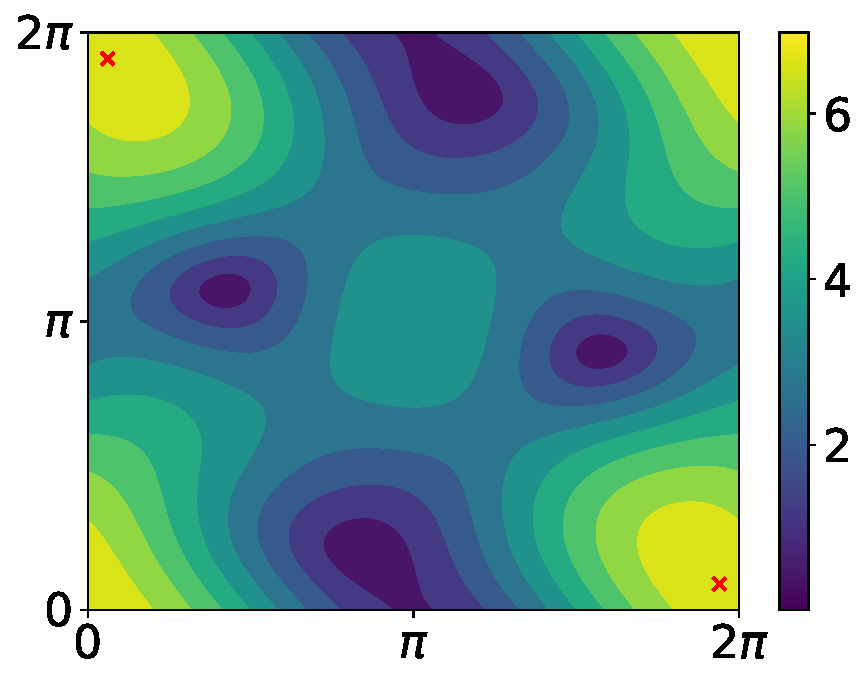
\includegraphics[scale=0.23]{figures/chapter4/contour_poly_200_1_1_3.pdf}\\kernel $1\times3\times3$
  \end{minipage}
  \begin{minipage}{.24\linewidth}
      \centering
      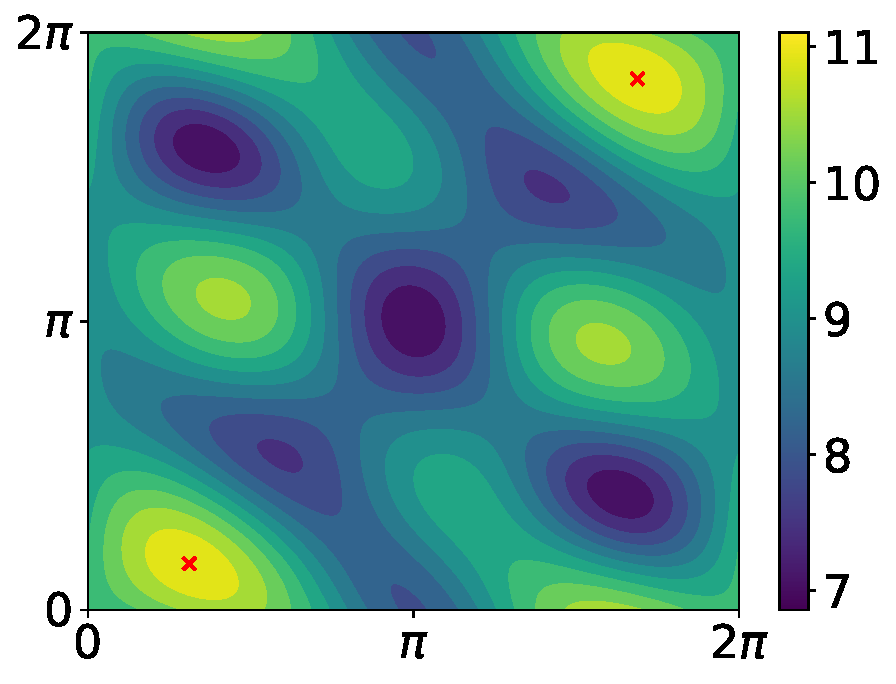
\includegraphics[scale=0.23]{figures/chapter4/contour_poly_200_1_9_3.pdf}\\kernel $9\times3\times3$
  \end{minipage}
  \begin{minipage}{.24\linewidth}
      \centering
      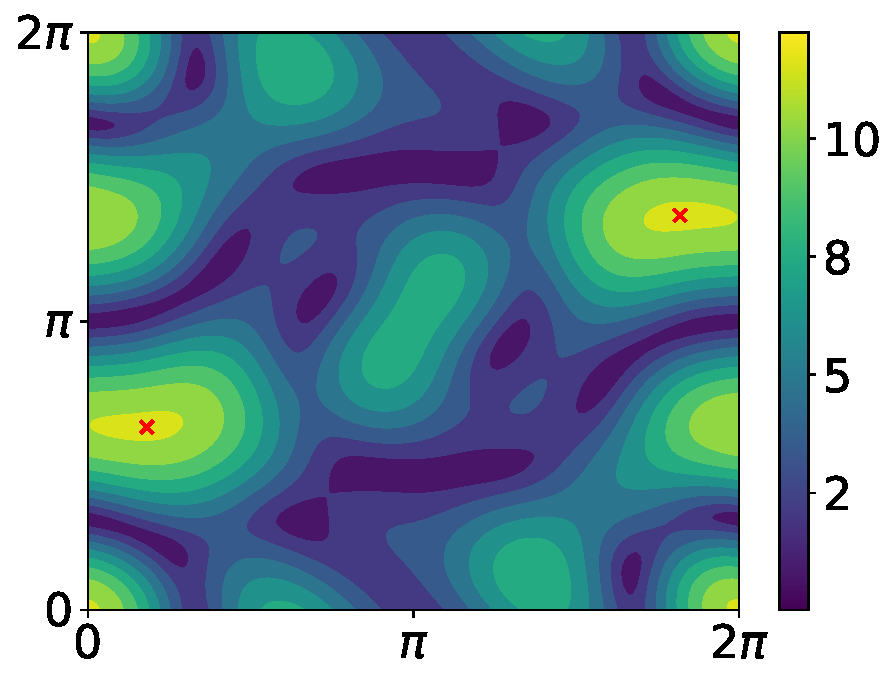
\includegraphics[scale=0.23]{figures/chapter4/contour_poly_200_1_1_5.pdf}\\kernel $1\times5\times5$
  \end{minipage}
  \begin{minipage}{.24\linewidth}
      \centering
      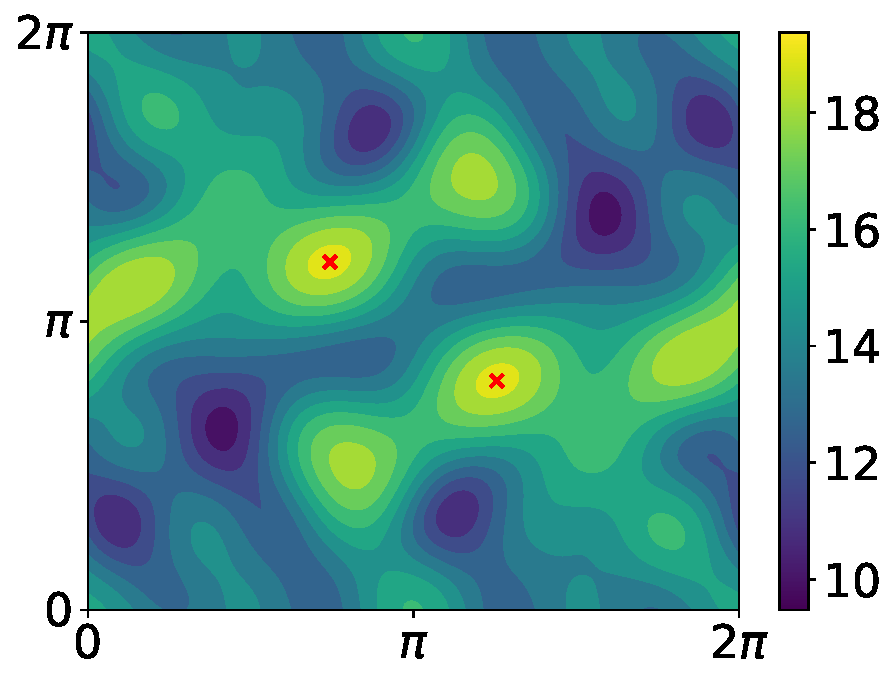
\includegraphics[scale=0.23]{figures/chapter4/contour_poly_200_1_9_5.pdf}\\kernel $9\times5\times5$
  \end{minipage}
  \caption{These figures represent the contour plot of multivariate trigonometric polynomials where the values of the coefficient are the values of a random convolutional kernel. The red dots in the figures represent the maximum modulus of the trigonometric polynomials.}
  \label{figure:contour_plot_trigonometric_polynomials}
\end{figure*}%

\begin{algorithm}
  \caption{PolyGrid Algorithm} \label{algorithm:PolyGrid}
  \begin{algorithmic}[1]
    \Procedure{PolyGrid}{$f, S$}\Comment{polynomial $f$, number of samples $S$}
      \State $\sigma \gets 0$, 
      \State $\omega_1 \gets 0$
      \State $\omega_2 \gets 0$
      \State $\epsilon \gets \frac{2\pi}{S}$
      \For{$i=0$ \textbf{to} $S-1$}
	\For{$j=0$ \textbf{to} $S-1$}
	  \State $\omega_2 \gets \omega_2 + \epsilon$
	  \State $\sigma \gets \max( \sigma, f(\omega_1, \omega_2))$
	\EndFor
      \EndFor
      \State \textbf{return} $\sigma$ \Comment{approximated maximum modulus of $f$}
    \EndProcedure
  \end{algorithmic}
\end{algorithm}

In order to compute $\lipbound$ from Theorem~\ref{theorem:bound_max_sv_convolution}, we have to compute the maximum modulus of several trigonometric polynomials.
However, finding the maximum modulus of a trigonometric polynomial has been known to be NP-Hard~\cite{pfister2018bounding}, and in practice they exhibit low convexity (see Figure~\ref{figure:contour_plot_trigonometric_polynomials}).
We found that for 2-dimensional kernels, a simple grid search algorithm such as PolyGrid (see Algorithm~\ref{algorithm:PolyGrid}), works better than more sophisticated approximation algorithms (\eg ~\citet{green1999calculating,de2009finding}).
This is because the complexity of the computation depends on the degree of the polynomial which is equal to $\lfloor s / 2 \rfloor$ where $s$ is the size of the kernel and is usually small in most practical settings (\eg $s=3$).
Furthermore, the grid search algorithm can be parallelized effectively on CPUs or GPUs and runs within less time than alternatives with lower asymptotic complexity. 

To fix the number of samples $S$ in the grid search, we rely on the work of~\cite{pfister2018bounding}, who has analyzed the quality of the approximation depending on $S$.
Following, this work we first define $\Theta_S$, the set of $S$ equidistant sampling points as follows:
\begin{equation}
  \Theta_S \triangleq \left\{ \omega \mid \omega = k \cdot \frac{2\pi}{S} \mbox{ with }  k = 0,\ldots, S-1 \right\}.
\end{equation}
Then, for a trigonometric polynomial $f: [0, 2\pi]^2 \rightarrow \mathbb{C}$, we have:
\begin{equation}
  \max_{\omega_1, \omega_2 \in [0,2\pi]^2} \left| f(\omega_1, \omega_2) \right| \leq (1 - \alpha)^{-1} \max_{\omega_1', \omega_2' \in \Theta_S^2} \left| f(\omega_1', \omega_2') \right|,
\end{equation}
where $d$ is the degree of the polynomial and $\alpha = 2d / S$.
For a $3\times3$ kernel which gives a trigonometric polynomial of degree 1, we use $S = 10$ which gives $\alpha = 0.2$.
Using this result, we can now compute $\lipbound$ for a convolution operator with $cout$ output channels as per Theorem~\ref{theorem:bound_sv_stacked_dbt}.
 
% The code to for computing $\lipbound$ with NumPy~\cite{numpy} and PyTorch~\cite{paszke2019pytorch} is publicly available.\footnote{\url{https://github.com/MILES-PSL/upper_bound_lipschitz_convolutional_layers}}.


\subsection{Analysis of the tightness of the bound}
\label{section:analysis_tightness_bound}

In this section, we study the tightness of the bound with respect to the dimensions of the doubly-block Toeplitz matrices.
For each $n \in \mathbb{N}$, we define the matrix  $\Mmat^{(n)}$ of size $kn^2 \times n^2$ as follows:
\begin{equation}
  \Mmat^{(n)} \triangleq \textstyle \leftmat \Dmat^{(n)\top}(f_1), \dots, \Dmat^{(n)\top}(f_k) \textstyle \rightmat^\top
\end{equation}
where the matrices $\Dmat^{(n)}(f_i)$ are of size $n^2 \times n^2$. 
To analyze the tightness of the bound, we define the function $\Gamma$, which computes the difference between $\lipbound$ and the maximal singular value of the function $\Mmat^{(n)}$:
\begin{equation} \label{equation:function_convergence}
  \Gamma(n) = \lipbound(\mathbf{k}_{\Mmat^{(n)}}) - \sigma_1(\Mmat^{(n)})
\end{equation}
where $\mathbf{k}_{\Mmat^{(n)}}$ is the  convolution kernel of the convolution defined by the matrix $\Mmat^{(n)}$.

\begin{figure}[ht]
  \centering
  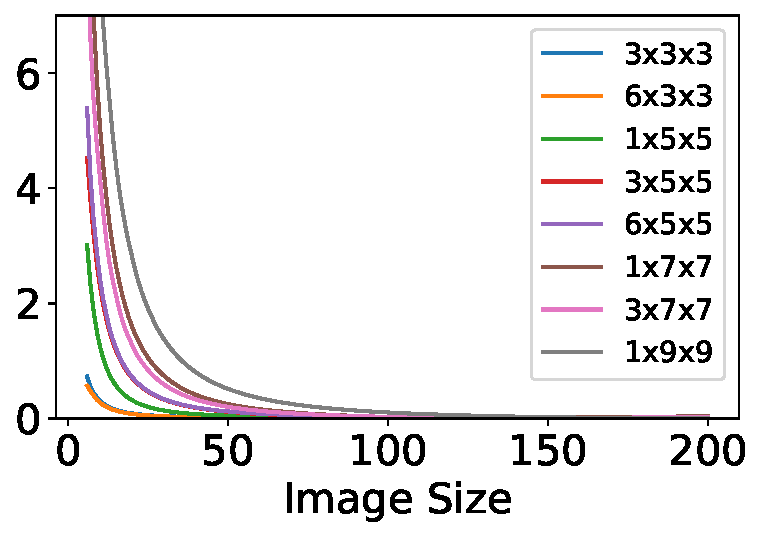
\includegraphics[scale=0.50]{figures/chapter4/convergence_bound.pdf}
  \caption{This graph represents the function $\Gamma(n)$ defined in Section~\ref{section:analysis_tightness_bound} for different kernel size.}
  \label{figure:convergence_bound}
\end{figure}


To compute the exact largest singular value of $\Mmat^{(n)}$ for a specific $n$, we use the Implicitly Restarted Arnoldi Method (IRAM) ~\cite{lehoucq1996deflation} available in SciPy.
The results of this experiment are presented in Figure~\ref{figure:convergence_bound}.
We observe that the difference between the bound and the actual value (approximation gap) quickly decreases as the input size increases.
For an input size of $50$, the approximation gap is as low as $0.012$ using a standard $6\times3\times3$ convolution kernel.
For a larger input size such as ImageNet ($224$), the gap is lower than $4.10^{-4}$.
Therefore $\lipbound$ gives an almost exact value of the maximal singular value of the operator matrix for most realistic settings.

\subsection{Comparison of LipBound with other state-of-the-art approaches} \label{subsection:comparaison_sota}

\begin{table}[ht]
  \centering
  \caption{The following table compares different approaches for computing an approximation of the maximal singular value of a convolutional layer. It shows the ratio between the approximation and the true maximal singular value. The approximation is better for a ratio close to one.}
  {\footnotesize
    \begin{tabular}{lrccrcc}
    \toprule
      &   & \multicolumn{2}{c}{\textbf{1x3x3}} &   & \multicolumn{2}{c}{\textbf{32x3x3}} \\
    \cmidrule{3-4}\cmidrule{6-7}  &   & \textbf{Ratio} & \textbf{Time (ms)} &   & \textbf{Ratio} & \textbf{Time (ms)} \\
    \midrule
    \citeauthor{sedghi2018iclr} &   & $\phantom{.}0.431\pm0.042$ & $1088\pm251$ &   & $\phantom{.}0.666\pm0.123$ & $1729\pm399$ \\
    \citeauthor{singla2019bounding} &   & $\phantom{.}1.293\pm0.126$ & $\phantom{..}1.90\pm0.48$ &   & $\phantom{.}1.441\pm0.188$ & $\phantom{..}1.90\pm0.46$ \\
    \citeauthor{farnia2018generalizable} (10 iter) &   & $\phantom{.}0.973\pm0.006$ & $\phantom{..}4.30\pm0.64$ &   & $\phantom{.}0.972\pm0.004$ & $\phantom{..}4.93\pm0.67$ \\
    \midrule
    \midrule
    \textbf{LipBound (Ours)} &   & $\mathbf{0.992}\pm0.012$ & $\phantom{.}\mathbf{0.49}\pm0.05$ &   & $\mathbf{0.984}\pm0.021$ & $\phantom{.}\mathbf{0.63}\pm0.46$ \\
    \bottomrule
    \end{tabular}%
  }
  \label{table:comparaison}%
\end{table}


In this section we compare our PolyGrid algorithm with the values obtained using alternative approaches.
We consider the 3 alternative techniques by~\citet{sedghi2018iclr,singla2019bounding,farnia2018generalizable} which have been described in Section~\ref{section:ch4-related_work}. 

To compare the different approaches, we extracted 20 kernels from a trained model.
For each kernel we construct the corresponding doubly-block Toeplitz matrix and compute its largest singular value.
Then, we compute the ratio between the approximation obtained with the approach in consideration and the exact singular value obtained by SVD, and average the ratios over the 20 kernels.
Thus good approximations result in approximation ratios that are close to 1.
The results of this experiment are presented in Table~\ref{table:comparaison}.
The comparison has been made on a Tesla V100 GPU. 
The time was computed with the PyTorch CUDA profiler and we warmed up the GPU before starting the timer.

The method introduced by~\citet{sedghi2018iclr} computes an approximation of the singular values of convolutional layers.
We can see in Table~\ref{table:comparaison} that the value is off by an important margin.
This technique is also computationally expensive as it requires computing the SVD of $n^2$ small matrices where $n$ is the size of inputs.
\citet{singla2019bounding} have shown that the singular value of the reshape kernel is a bound on the maximal singular value of the convolution layer.
Their approach is very efficient but the approximation is loose and overestimate the real value.
As said previously, the power method provides a good approximation at the expense of the efficiency.
We use the special Convolutional Power Method from~\citet{farnia2018generalizable} with 10 iterations.
The results show that our proposed technique: PolyGrid algorithm can get the best of both worlds.
It achieves a near perfect accuracy while being very efficient to compute. 

We provide in the supplementary material a benchmark on the efficiency of $\lipbound$ on multiple convolutional architectures. 


%%%%%%%%%%%%%%%%%%%%%%%%%%%%%%%%%%%%%%%%%%%%%%%%%%%%%%%%%%%%%%%%%%%%%%%%%%%%%%%
\section{Application: Lipschitz Regularization for Adversarial Robustness}
\label{section:experiments}
%%%%%%%%%%%%%%%%%%%%%%%%%%%%%%%%%%%%%%%%%%%%%%%%%%%%%%%%%%%%%%%%%%%%%%%%%%%%%%%

\begin{table}[t]
  \centering
  \caption{This table shows the Accuracy under $\ltwo$ and $\linf$ attacks of CIFAR10 dataset. We compare vanilla Adversarial Training with the combination of Lipschitz regularization and Adversarial Training. We also compare the effectiveness of the power method by~\citet{farnia2018generalizable} and $\lipbound$. The parameters $\lambda_2$ from Equation~\ref{equation:objectif_function} is equal to $0.008$ for AT+PM and AT+LipReg. It has been chosen from a grid search among 10 values. The attacks below are computed with 200 iterations. }
    \begin{tabular}{lcccc}
    \toprule
      & \textbf{Accuracy} & \textbf{PGD-$\linf$} & \textbf{C\&W-$\ltwo$ 0.6} & \textbf{C\&W-$\ltwo$ 0.8} \\
    \midrule
    \textbf{Baseline} & $\mathbf{0.953}\pm0.001$ & $\phantom{.}0.000\pm0.000$ & $\phantom{.}0.002\pm0.000$ & $\phantom{.}0.000\pm0.000$ \\
    \textbf{AT} & $\phantom{.}0.864\pm0.001$ & $\phantom{.}0.426\pm0.000$ & $\phantom{.}0.477\pm0.000$ & $\phantom{.}0.334\pm0.000$ \\
    \textbf{AT+PM} & $\phantom{.}0.788\pm0.010$ & $\phantom{.}0.434\pm0.007$ & $\phantom{.}0.521\pm0.005$	 & $\phantom{.}0.419\pm0.003$ \\
    \textbf{AT+LipReg} & $\phantom{.}0.808\pm0.022$ & $\mathbf{0.457}\pm0.002$ & $\mathbf{0.547}\pm0.022$ & $\mathbf{0.438}\pm0.020$ \\
    \bottomrule
    \end{tabular}%
  \label{tab:table_cifar10_robustness}%
\end{table}%

One promising application of Lipschitz regularization is in the area of adversarial robustness.
Empirical techniques to improve robustness against adversarial examples such as Adversarial Training only impact the training data,  and often show poor generalization capabilities~\cite{schmidt2018adversarially}. 
\citet{farnia2018generalizable} have shown that the adversarial generalization error depends on the Lipschitz constant of the network, which suggests that the adversarial test error can be improved by applying Lipschitz regularization in addition to adversarial training. 

In this section, we illustrate the usefulness of LipBound by training a state-of-the-art Wide ResNet architecture~\cite{zagoruyko2016wide} with Lipschitz regularization and adversarial training.
Our regularization scheme is inspired by the one used by~\citet{yoshida2017spectral} but instead of using the power method, we use our \textbf{PloyGrid} algorithm presented in Section~\ref{subsection:computing_max_modulus_trig_polynomial} which efficiently computes an upper bound on the maximal singular value of convolutional layers. 

We introduce the \textbf{AT+LipReg} loss to combine Adversarial Training and our Lipschitz regularization scheme in which layers with a large Lipschitz constant are penalized.
We consider a neural network $\mathcal N_\theta : \mathcal X \rightarrow \mathcal Y$ with $\ell$ layers $\phi^{(1)}_{\theta_1}, \ldots, \phi^{(\ell)}_{\theta_\ell}$ where $\theta^{(1)}, \ldots, \theta^{(\ell -1)}$ are the kernels of the first $\ell - 1$ convolutional layers and $\theta_\ell$ is the weight matrix of the last fully-connected  layer $\phi^{(\ell)}_{\theta_\ell}$.
Given a distribution $\mathcal D$ over $\mathcal X \times \mathcal Y$, we can train the parameters $\theta$ of the network by minimizing the AT+LipReg loss as follows:
\begin{equation} \label{equation:objectif_function}
    \min_{\theta} \mathbb E_{x,y \sim \mathcal D} \left[ \max_{\norm{\tau}_\infty \leq \epsilon} \mathcal{L}(\mathcal{N}_\theta(x + \tau), y)  + \lambda_1 \sum_{i=1}^\ell {\textstyle \norm{\theta_i}_\text{F}} + \lambda_2 \sum_{i=1}^{\ell-1} \log\left( \lipbound\left(\theta_i\right)\right) \right]
\end{equation}
where $\mathcal L$ is the cross-entropy loss function, and $\lambda_1$, $\lambda_2$ are two user-defined hyper-parameters.
Note that regularizing the sum of logs is equivalent to regularizing the product of all the $\lipbound$ which is an upper bound on the global Lipschitz constant.
In practice, we also include the upper bound on the Lipschitz of the batch normalization because we can compute it very efficiently (see C.4.1 of~\citet{tsuzuku2018lipschitz}) but we omit the last fully connected layer. 

\begin{figure}[ht]
   \centering
   \begin{subfigure}[b]{0.49\textwidth}
       \centering
       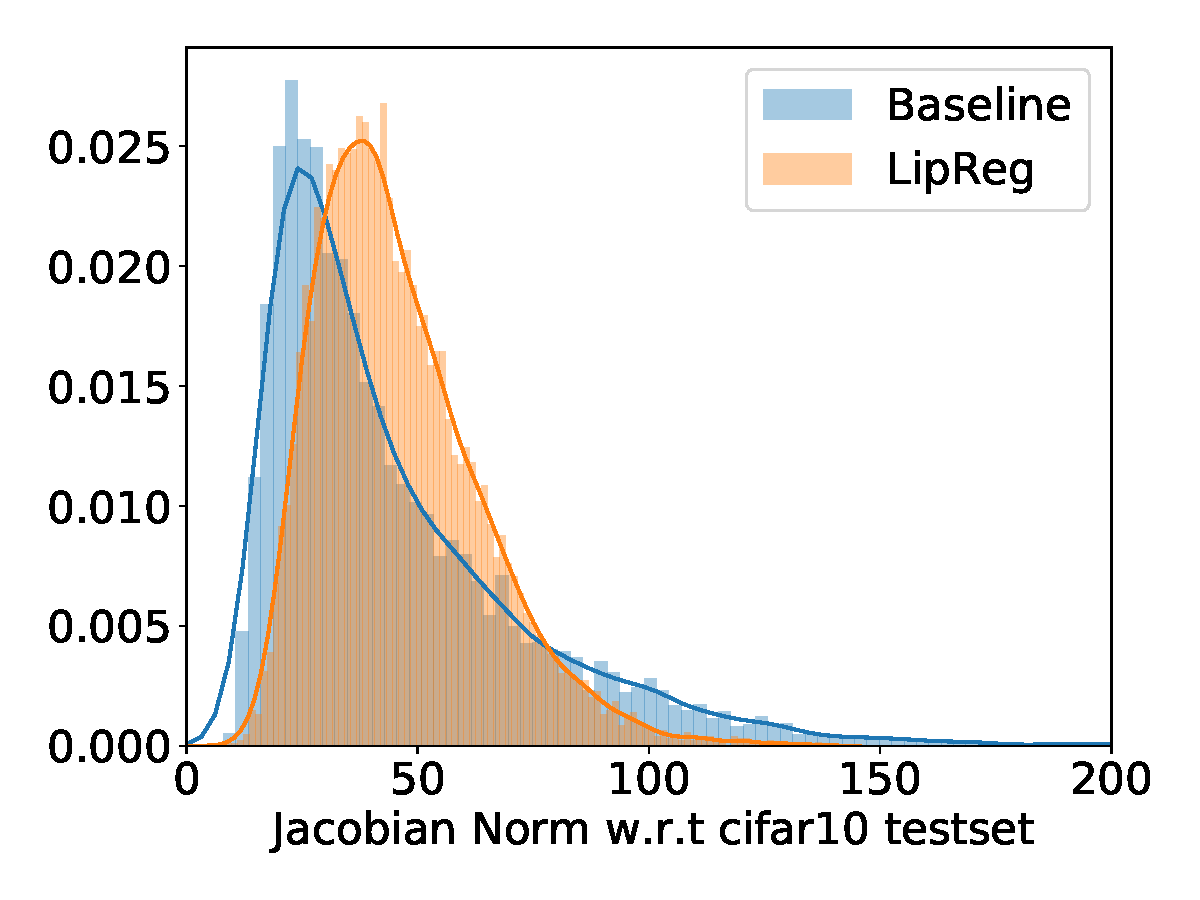
\includegraphics[width=\textwidth]{figures/chapter4/jacobian_distribution_v1.pdf}\\(a)
   \end{subfigure}
   \hfill
   \begin{subfigure}[b]{0.49\textwidth}
       \centering
       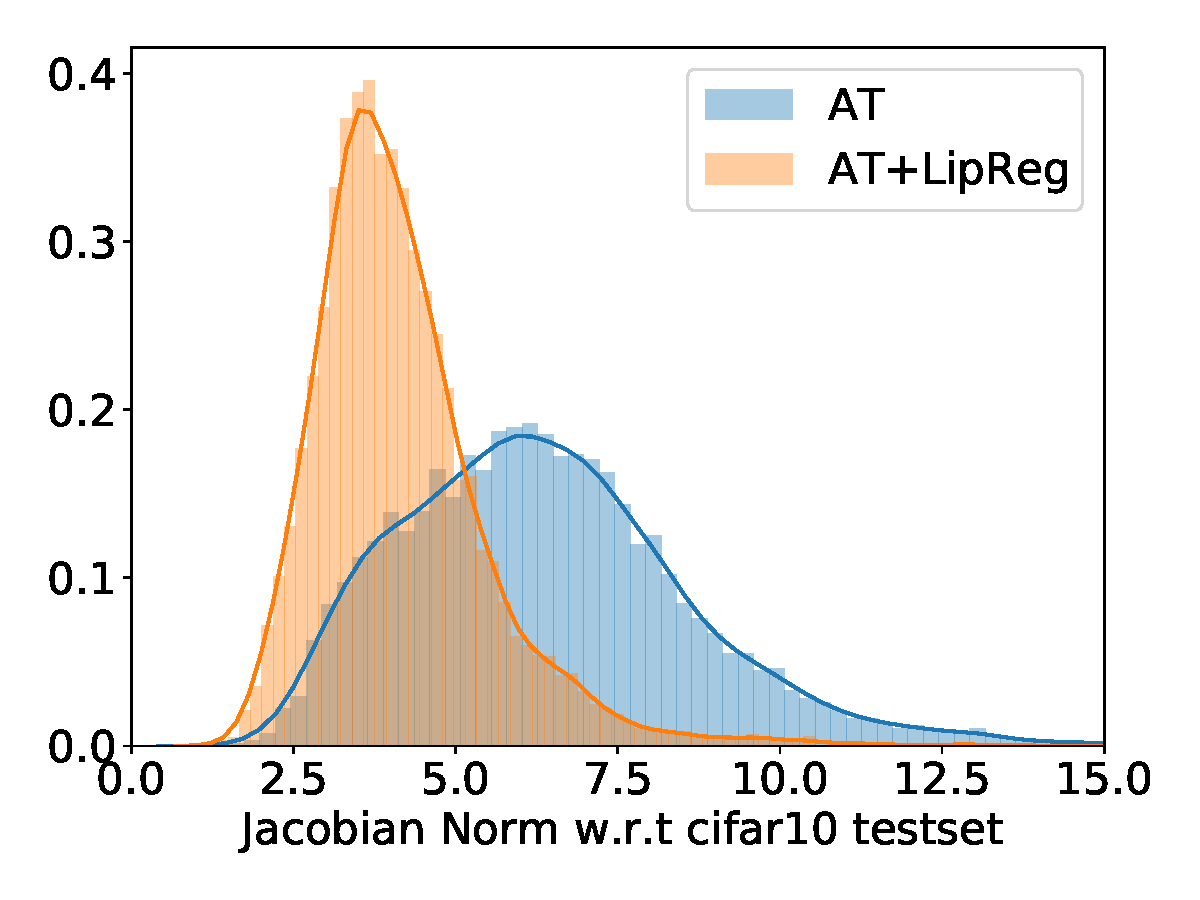
\includegraphics[width=\textwidth]{figures/chapter4/jacobian_distribution_v2.pdf}\\(b)
   \end{subfigure}
   \caption{These figures show the distribution of the norm of the Jacobian matrix w.r.t the CIFAR10 test set from a Wide Resnet trained with different schemes. Although Lipschitz regularization is not a Jacobian regularization, we can observe a clear shift in the distribution. This suggests that our method does not only work layer-wise, but also at the level of the entire network.}
   \label{figure:jacobian_distribution}
\end{figure}


\begin{figure}[ht]
   \centering
   \begin{subfigure}[b]{0.49\textwidth}
       \centering
       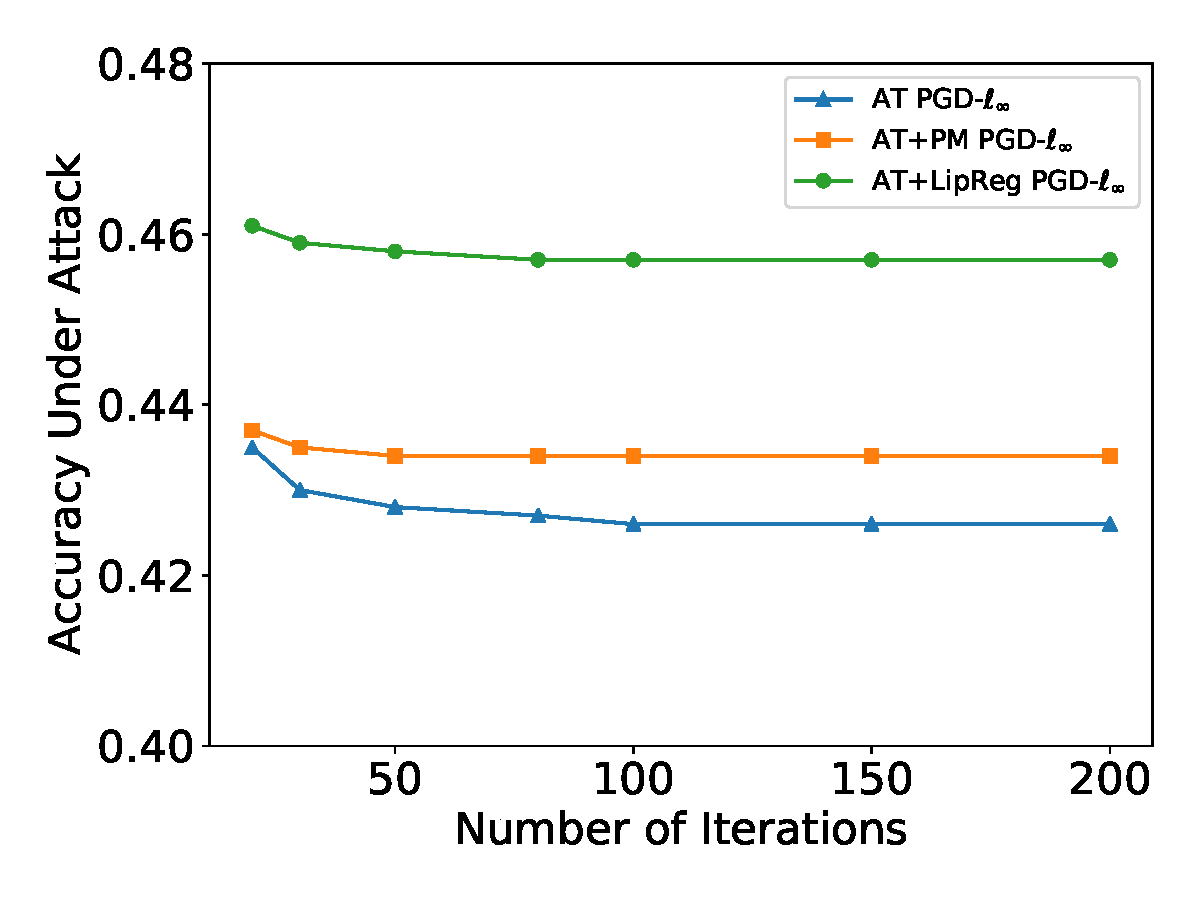
\includegraphics[width=\textwidth]{figures/chapter4/attacks_iter_pgd.pdf}\\(a)
   \end{subfigure}
   \hfill
   \begin{subfigure}[b]{0.49\textwidth}
       \centering
       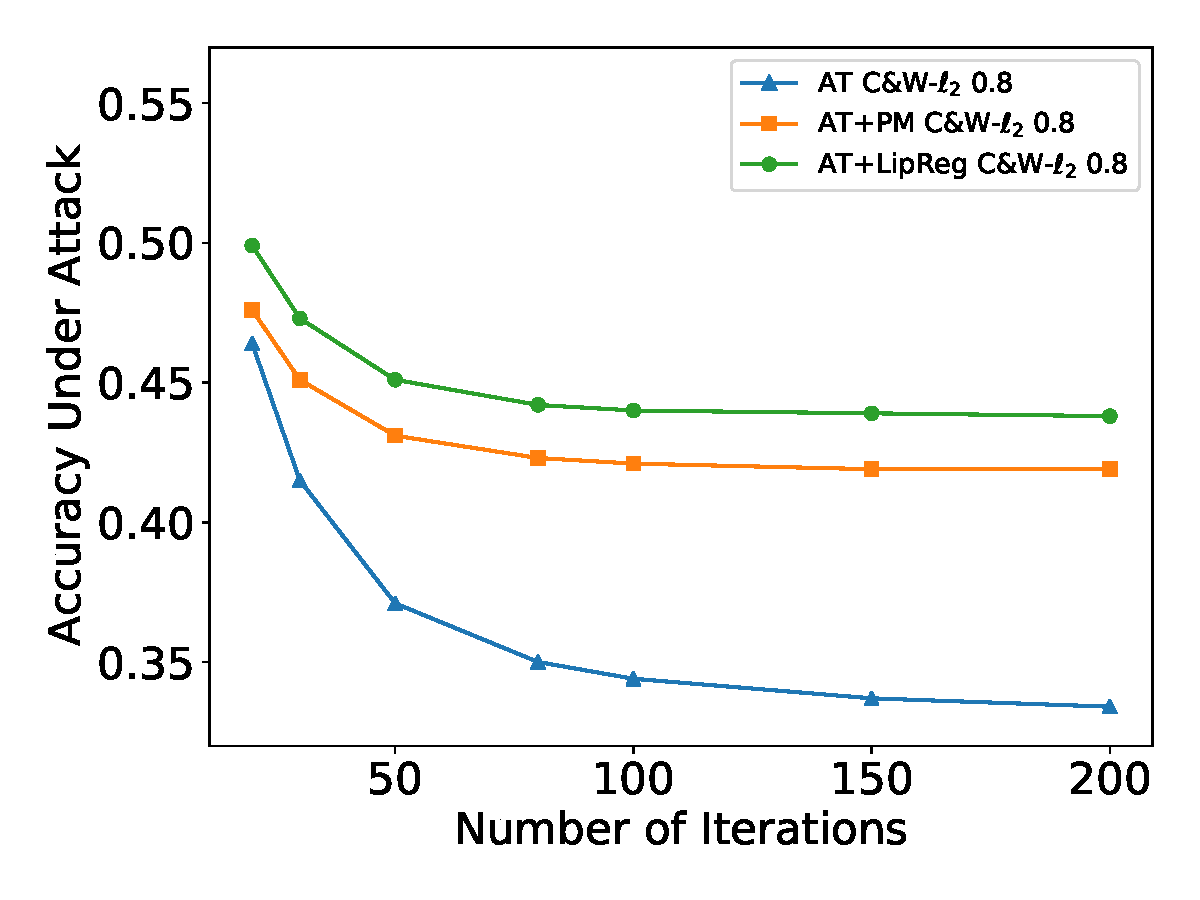
\includegraphics[width=\textwidth]{figures/chapter4/attacks_iter_cw.pdf}\\(b)
   \end{subfigure}
   \caption{These figures show the Accuracy under attack on CIFAR10 test set with PGD-$\linf$ and C\&W-$\ltwo$ attacks for several classifiers trained with Adversarial Training given the number of iterations.}
   \label{figure:attacks_iter}
\end{figure}


% \begin{figure*}[htb]
%   \centering
%   \begin{minipage}{.24\linewidth}
%     \centering
%     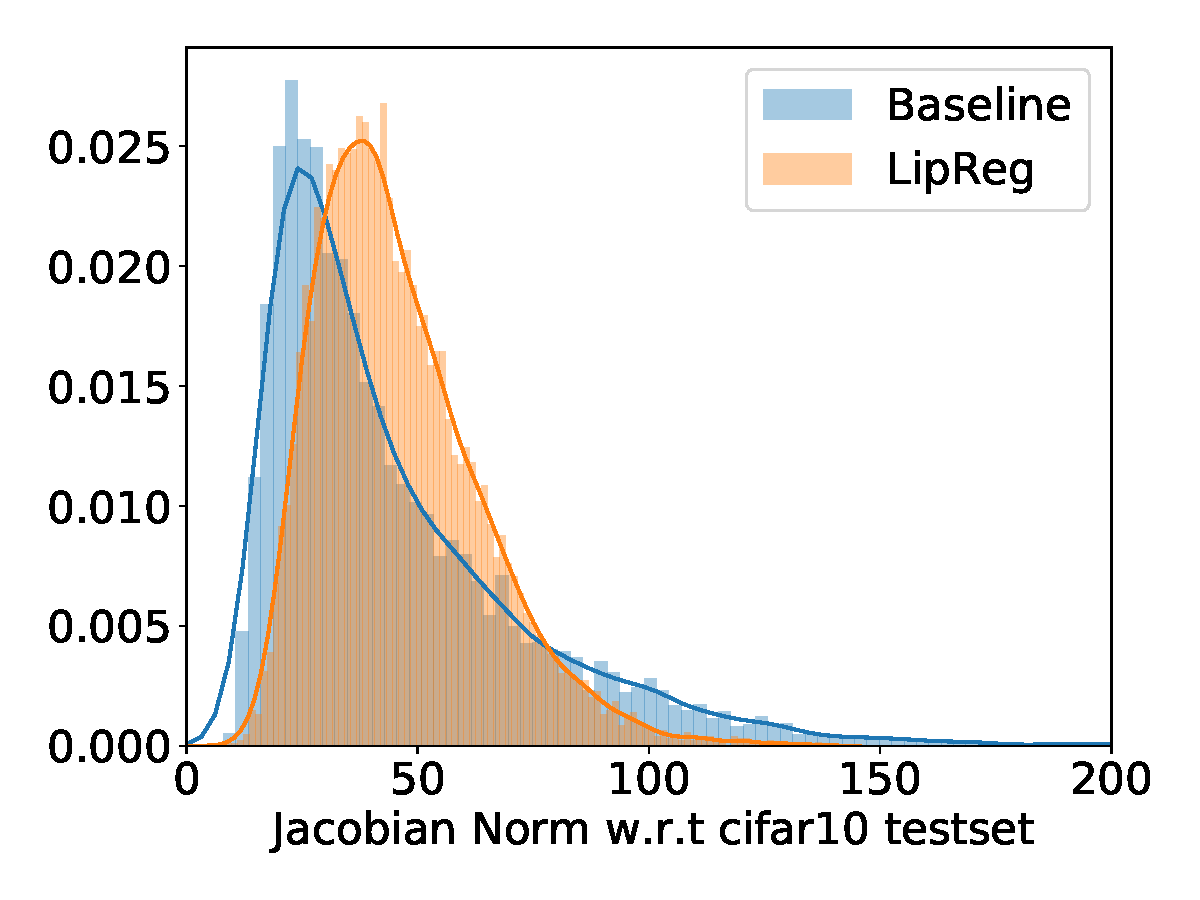
\includegraphics[scale=0.16]{figures/chapter4/jacobian_distribution_v1.pdf}\\{(a)}
%   \end{minipage}
%   \hfill
%   \begin{minipage}{.24\linewidth}
%     \centering
%     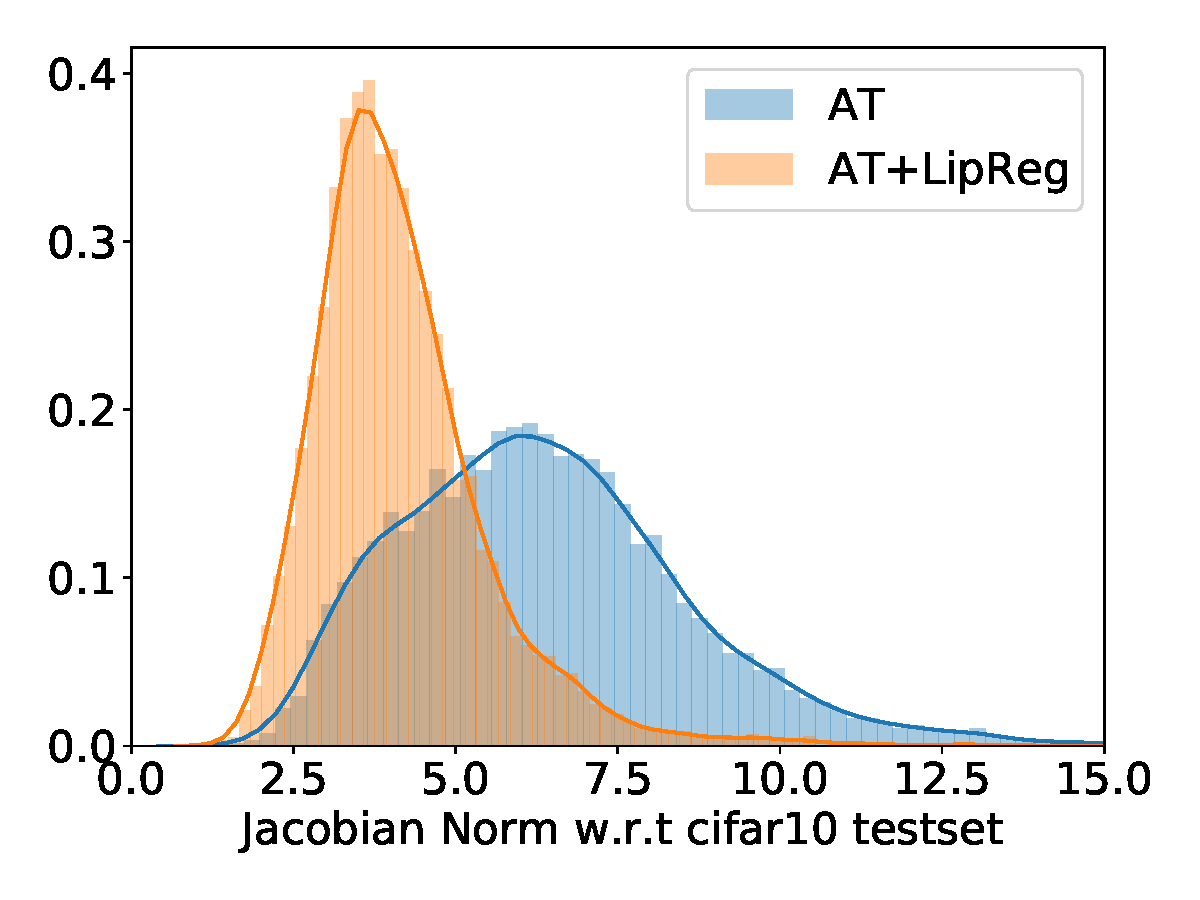
\includegraphics[scale=0.16]{figures/chapter4/jacobian_distribution_v2.pdf}\\{(b)}
%   \end{minipage}
%   \hfill
%   \begin{minipage}{.24\linewidth}
%     \centering
%     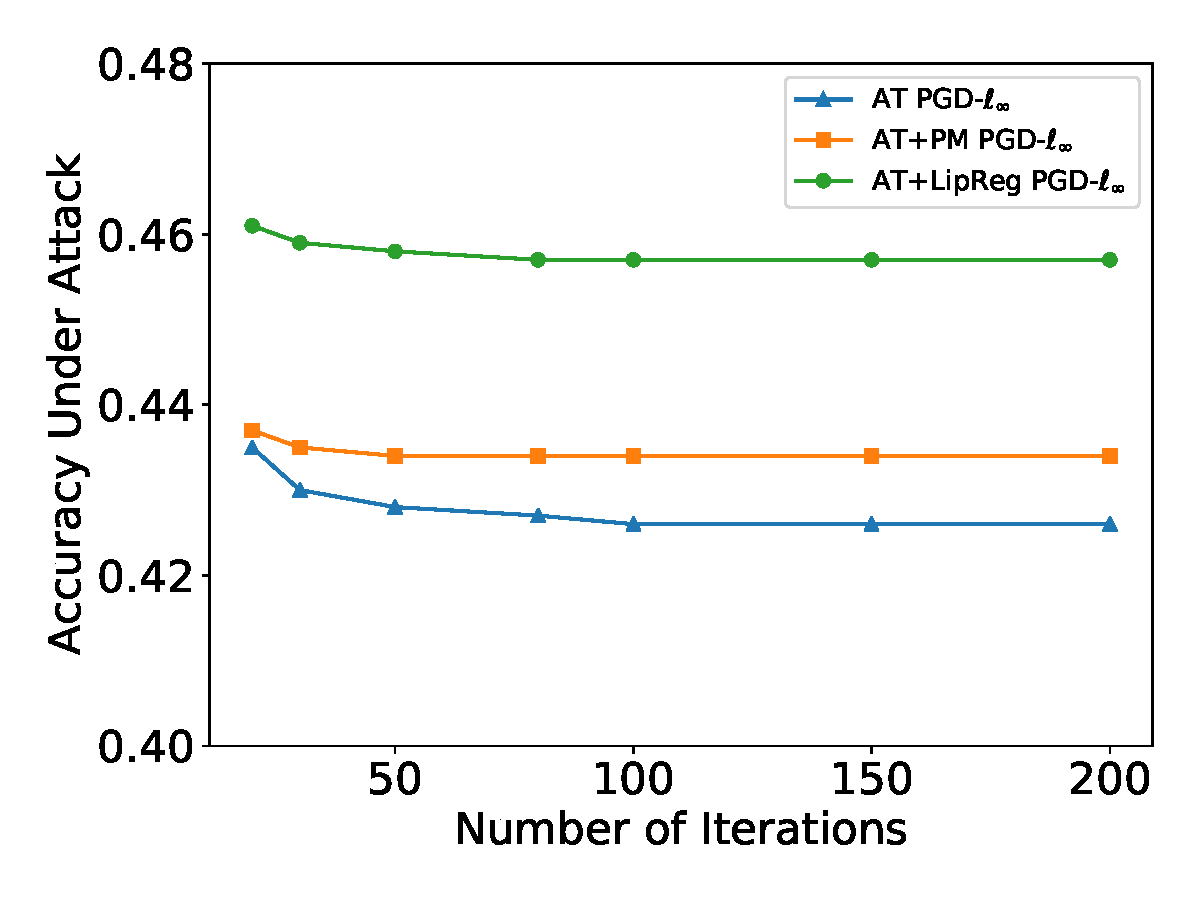
\includegraphics[scale=0.16]{figures/chapter4/attacks_iter_pgd.pdf}\\{(c)}
%   \end{minipage}
%   \hfill
%   \begin{minipage}{.24\linewidth}
%     \centering
%     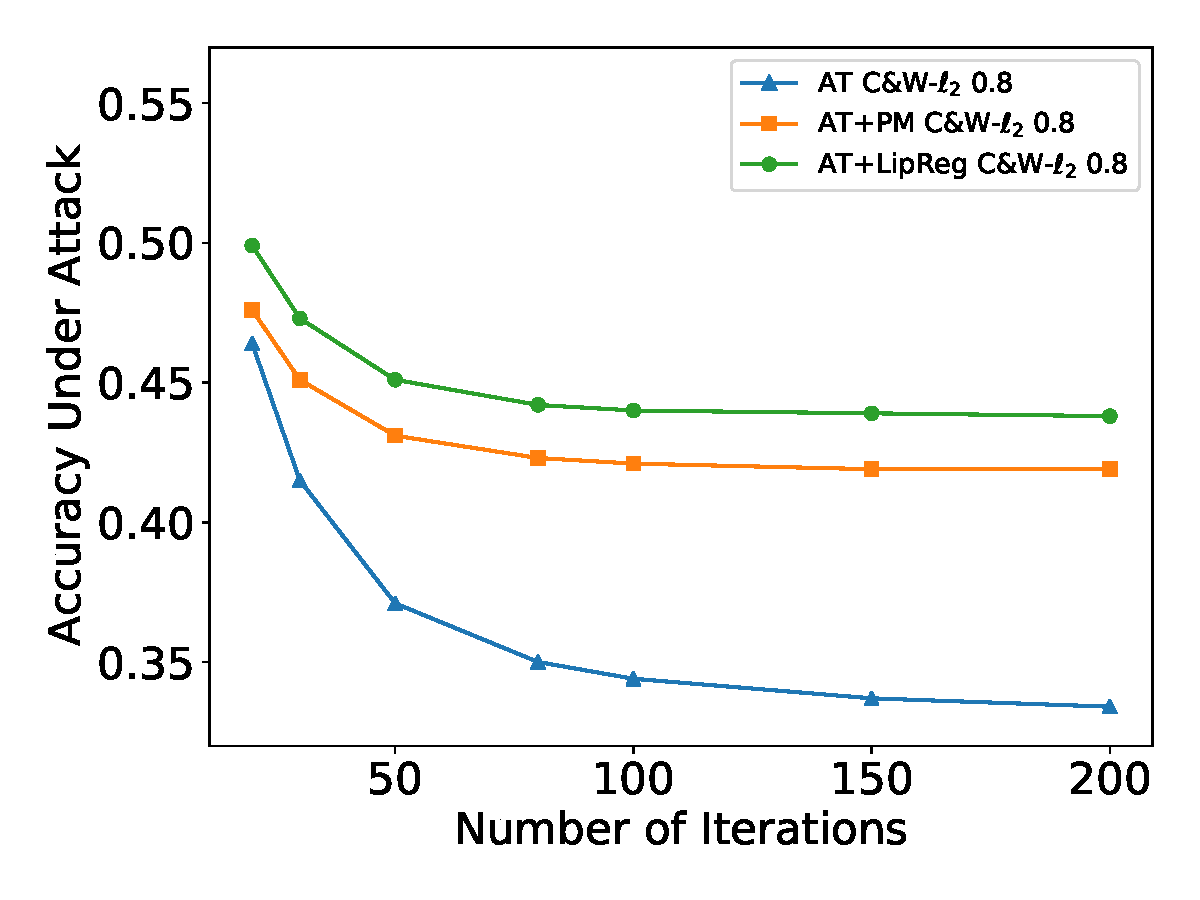
\includegraphics[scale=0.16]{figures/chapter4/attacks_iter_cw.pdf}\\{(d)}
%   \end{minipage}
%   \caption{Figures (a) and (b) show the distribution of the norm of the Jacobian matrix w.r.t the CIFAR10 test set from a Wide Resnet trained with different schemes. Although Lipschitz regularization is not a Jacobian regularization, we can observe a clear shift in the distribution. This suggests that our method does not only work layer-wise, but also at the level of the entire network. Figures (c) and (d) show the Accuracy under attack on CIFAR10 test set with PGD-$\linf$ and C\&W-$\ltwo$ attacks for several classifiers trained with Adversarial Training given the number of iterations.}
%   \label{figure:dist_jacobian_attacks_iter}
% \end{figure*}%


In this section, we compare the robustness of Adversarial Training~\cite{goodfellow2014explaining, madry2018towards} against the combination of Adversarial Training and Lipschitz regularization.
To regularize the Lipschitz constant of the network, we use the objective function defined in Equation~\ref{equation:objectif_function}.
We train Lipschitz regularized neural network with LipBound (Theorem~\ref{theorem:bound_max_sv_convolution}) implemented with PolyGrid (Algorithm~\ref{algorithm:PolyGrid}) (AT+LipBound) with $S = 10$ or with the specific power method for convolutions introduced by~\citet{farnia2018generalizable} with 10 iterations (AT+PM). 

Table~\ref{tab:table_cifar10_robustness} shows the gain in robustness against strong adversarial attacks.
We can observe that both AT+LipBound and AT+PM offer a better defense against adversarial attacks and that AT+LipBound offers a further improvement over the Power Method.
The Figure~\ref{figure:attacks_iter} (b) shows the Accuracy under attack with different number of iterations. 

Finally, we also conducted an experiment to study the impact of the regularization on the gradients of the whole network by measuring the norm of the Jacobian matrix, averaged over the inputs from the test set.
The results of this experiment are presented in Figure~\ref{figure:jacobian_distribution} (a) and show more concentrated gradients with Lipschitz regularization, which is the expected effect.
This suggests that our method does not only work layer-wise, but also at the level of the entire network.
A second experiment, using Adversarial Training, presented in Figure~\ref{figure:jacobian_distribution} (b) demonstrates that the effect is even stronger when the two techniques are combined together.
This corroborates the work by~\cite{farnia2018generalizable}.
It also demonstrates that Lipschitz regularization and Adversarial Training (or other Jacobian regularization techniques) are complementary.
Hence they offer an increased robustness to adversarial attacks as demonstrated above.

\paragraph{Experimental Settings}
We use the Wide ResNet architecture introduced by~\citet{zagoruyko2016wide} to train our classifiers (for details of the hyper-parameters used, see the supplementary material).
For Adversarial Training ~\cite{madry2018towards}, we use Projected Gradient Descent with an $\epsilon = 8/255 (\approx 0.031)$, a step size of $\textstyle \frac{\epsilon}{5} (\approx 0.0062)$ and 10 iterations, we use a random initialization but run the attack only once.
To evaluate the robustness of our classifiers, we rigorously followed the experimental protocol proposed by~\citet{tramer2020adaptive} and~\citet{carlini2019evaluating}.
More precisely, as an $\linf$ attack, we use PGD with the same parameters ($\epsilon = 8/255$, a step size of $\textstyle \frac{\epsilon}{5}$) but we increase the number of iterations up to 200 with 10 restarts.
For each image, we select the perturbation that maximizes the loss among all the iterations and the 10 restarts.
As $\ltwo$ attacks, we use a bounded version of the~\cite{carlini2017towards} attack.
We choose $0.6$ and $0.8$ as bounds for the $\ltwo$ perturbation. Note that the $\ltwo$ ball with a radius of $0.8$ has approximately the same volume as the $\linf$ ball with a radius of $0.031$ for the dimensionality of CIFAR10. 


\subsection{Results on CIFAR100 dataset \& Hyper-parameters}

\begin{table}[htb]
  \centering
  \caption{This table shows the Accuracy under $\ltwo$ and $\linf$ attacks of CIFAR100 dataset. We compare Adversarial Training with the combination of Lipschitz regularization and Adversarial Training \cite{madry2018towards}. The $\lambda_2$ parameters which control the Lipschitz regularization is $0.008$, it has been chosen among a grid search of 10 values. The attacks below are computed with 200 iterations.}
    \begin{tabular}{lcccc}
    \toprule
      & \textbf{Accuracy} & \textbf{PGD-$\linf$} & \textbf{C\&W-$\ltwo$ 0.6} & \textbf{C\&W-$\ltwo$ 0.8} \\
    \midrule
    \textbf{Baseline} & $\mathbf{0.792}\pm0.000$ & $\phantom{.}0.000\pm0.000$ & $\phantom{.}0.001\pm0.000$ & $\phantom{.}0.000\pm0.000$ \\
    \textbf{AT} & \phantom{.}$0.591\pm0.000$ & $\phantom{.}0.199\pm0.000$ & $\phantom{.}0.263\pm0.000$ & $\phantom{.}0.183\pm0.000$ \\
    \textbf{AT+LipReg} & \phantom{.}$0.552\pm0.019$ & $\mathbf{0.215}\pm0.004$ & $\mathbf{0.294}\pm0.010$ & $\mathbf{0.226}\pm0.008$ \\
    \bottomrule
    \end{tabular}%
  \label{tab:results_cifar100}%
\end{table}%


\paragraph{Hyper-parameters used for training classifiers on CIFAR10 \& CIFAR100 dataset}
For all our experiments, we use the Wide Resnet architecture \cite{zagoruyko2016wide} with 28 layers and a width factor of 10. We train our networks for 200 epochs with a batch size of $200$. We use Stochastic Gradient Descent with a momentum of $0.9$, an initial learning rate of $0.1$ with exponential decay of 0.1 (MultiStepLR gamma = 0.1) after the epochs $60$, $120$ and $160$. 

\subsection{Results on ImageNet dataset \& Hyper-parameters}

\begin{table}[htb]
  \centering
  \caption{This table shows the accuracy and accuracy under attack of ImageNet dataset with different training schemes. We compare Adversarial Training with the combination of Lipschitz regularization and Adversarial Training \cite{madry2018towards}. }
    {\footnotesize
    \begin{tabular}{lccccccccc}
    \toprule
      & \multicolumn{1}{c}{\multirow{2}[4]{*}{$\lambda_2$}} & \multicolumn{1}{c}{\multirow{2}[4]{*}{\textbf{Natural}}} &   & \multicolumn{2}{c}{\textbf{PGD-}$\linf$} &   & \multicolumn{3}{c}{\textbf{C\&W-}$\ltwo$} \\
\cmidrule{5-6}\cmidrule{8-10}      &   &   &   & \multicolumn{1}{c}{0.02} & \multicolumn{1}{c}{0.031} &   & \multicolumn{1}{c}{1.00} & \multicolumn{1}{c}{2.00} & \multicolumn{1}{c}{3.00} \\
    \midrule
    \textbf{AT} & \multicolumn{1}{c}{-} & 0.509 &   & 0.251 & 0.118 &   & 0.307 & 0.168 & 0.099 \\
    \textbf{AT+LipReg} & 0.0006 & \textbf{0.515} &   & \textbf{0.255} & \textbf{0.121} &   & \textbf{0.316} & \textbf{0.177} & \textbf{0.105} \\
    \textbf{AT+LipReg} & 0.0010 & \textbf{0.519} &   & \textbf{0.259} & \textbf{0.123} &   & \textbf{0.338} & \textbf{0.204} & \textbf{0.129} \\
    \bottomrule
    \end{tabular}%
    }
\end{table}%


\paragraph{Hyper-parameters used for training and attacking classifiers on ImageNet dataset}

For all our experiments, we use the Resnet-101 architecture \cite{he2016deep}. We have used Stochastic Gradient Descent with a momentum of $0.9$, a weight decay of $0.0001$, label smoothing of $0.1$, an initial learning rate of $0.1$ with exponential decay of $0.1$ (MultiStepLR gamma = $0.1$) after the epochs $30$ and $60$. We have used Exponential Moving Average over the weights with a decay of $0.999$. We have trained our networks for 80 epochs with a batch size of $4096$. For Adversarial Training, we have used PGD with 5 iterations, $\epsilon = 8/255 (\approx 0.031)$ and a step size of $\frac{\epsilon}{5} (\approx 0.0062)$. 

To evaluate the robustness of our classifiers in ImageNet, we have used an $\linf$ and an $\ltwo$ attacks. More precisely, as an $\linf$ attack, we use PGD with an epsilon of 0.02 and 0.031, a step size of $\textstyle \frac{\epsilon}{5}$) but we increase the number of iterations to 30 with 5 restarts. For each image, we select the perturbation that maximizes the loss among all the iterations and the 10 restarts. As $\ltwo$ attacks, we use a bounded version of the~\cite{carlini2017towards} attack. We have used $1$, $2$ and $3$ as bounds for the $\ltwo$ perturbation. 


%%%%%%%%%%%%%%%%%%%%%%%%%%%%%%%%%%%%%%%%%%%%%%%%%%%%%%%%%%%%%%%%%%%%%%%%%%%%%%%
\section{Conclusion}
\label{section:ch4-conclusion}
%%%%%%%%%%%%%%%%%%%%%%%%%%%%%%%%%%%%%%%%%%%%%%%%%%%%%%%%%%%%%%%%%%%%%%%%%%%%%%%

In this chapter, we introduced a new bound on the Lipschitz constant of convolutional layers that is both accurate and efficient to compute.
We used this bound to regularize the Lipschitz constant of neural networks and demonstrated its computational efficiency in training large neural networks with a regularized Lipschitz constant.
As an illustrative example, we   combined our bound with adversarial training, and showed that this increases the robustness of the trained networks to  adversarial attacks.
The scope of our results goes beyond this application and can be used  in a wide variety of settings, for example, to stabilize Generative Adversarial Networks, or improve generalization capabilities of classifiers, to mention a few.
Our future work will focus on investigating these fields. 



% \section{Notations}
% Below are the notations we will use for the theorems and proofs. 
% \begin{itemize}
% \itemsep0em 
%     \item Let $\ci = \sqrt{-1}$.
%     \item We denote $\sigma_1(\Amat) = \sigma_{max}(\Amat)$ the maximum singular value of the matrix $\Amat$. 
%     \item We denote $\lambda_1(\Amat) = \lambda_{max}(\Amat)$ the maximum eigenvalue of the Hermitian matrix $\Amat$. 
%     \item For any function $f: \mathcal{X} \rightarrow \mathbb{C}$, we denote $f^*$ the conjugate function of $f$.
%     \item Let $\Amat$ be a $n \times n$ symmetric real matrix, we say that 
%     \begin{itemize}
%         \item[] $\Amat$ is positive definite, and we note $\Amat > 0$ if $\mathbf{x}^{\top} \Amat \mathbf{x} > 0$ for all non-zero $\mathbf{x}$ in $\mathbb{R}^{n}$.
%         \item[] $\Amat$ is positive semi-definite, and we note $\Amat \geq 0$ if $\mathbf{x}^{\top} \Amat \mathbf{x} \geq 0$ for all non-zero $\mathbf{x}$ in $\mathbb{R}^{n}$.
%     \end{itemize}
%     \item Let $N = \{ -n+1, \dots, n-1 \}$ and $M = \{ -m+1, \dots, m-1 \}$
% \end{itemize}


% \section{Discussion on the Convolution Operation}



%
% \section{Additional Results and Discussions on the Experiments}
%
%
%
% \subsection{Additional Results and Discussion of Section~\ref{subsection:comparaison_sota}}
%
%
% \begin{table}[htb]
%   \centering
%   \caption{This table shows the efficiency of LipBound computation vs the Power Method with 10 iterations on the full networks.}
%   {\footnotesize
%     \begin{tabular}{llllr}
%     \toprule
%       &   & \multicolumn{1}{c}{\textbf{LipBound (ms)}} & \multicolumn{1}{c}{\textbf{Power Method (ms)}} & \textbf{Ratio} \\
%     \midrule
%      \cite{krizhevsky2012imagenet} & \textbf{AlexNet} & \phantom{....}$4.75\pm1.1$ & \phantom{....}$38.75\pm2.52$ & \textbf{8.14 }\\
%     \midrule
%     \multirow{5}[2]{*}{\cite{he2016deep}} & \textbf{ResNet 18} & \phantom{..}$29.88\pm1.73$ & \phantom{..}$148.35\pm14.92$ & \textbf{4.96 }\\
%       & \textbf{ResNet 34} & \phantom{..}$54.73\pm3.62$ & \phantom{..}$266.85\pm25.35$ & \textbf{4.87 }\\
%       & \textbf{ResNet 50} & \phantom{..}$60.77\pm4.62$ & \phantom{..}$467.61\pm36.52$ & \textbf{7.69 }\\
%       & \textbf{ResNet 101} & $102.72\pm11.53$ & \phantom{..}$817.06\pm102.87$ & \textbf{7.95 }\\
%       & \textbf{ResNet 152} & $158.80\pm20.84$ & $1373.57\pm164.37$ & \textbf{8.64} \\
%     \midrule
%     \multirow{4}[2]{*}{\cite{huang2017densely}} & \textbf{DenseNet 121} & $125.55\pm14.59$ & \phantom{..}$937.35\pm11.52$ & \textbf{7.46 }\\
%       & \textbf{DenseNet 161} & $176.11\pm19.13$ & $1292.61\pm30.5$ & \textbf{7.33} \\
%       & \textbf{DenseNet 169} & $188.03\pm19.74$ & $1372.62\pm21.16$ & \textbf{7.29} \\
%       & \textbf{DenseNet 201} & $281.13\pm23.41$ & $1930.19\pm170.79$ & \textbf{6.86 }\\
%     \midrule
%     \multirow{4}[2]{*}{\cite{simonyan2014very}} & \textbf{VGG 11} & \phantom{..}$13.73\pm1.19$ & \phantom{....}$81.78\pm4.45$ & \textbf{5.95 }\\
%       & \textbf{VGG 13} & \phantom{..}$14.96\pm1.99$ & \phantom{..}$102.04\pm4.2$ & \textbf{6.82 }\\
%       & \textbf{VGG 16} & \phantom{..}$21.92\pm1.94$ & \phantom{..}$132.29\pm5.99$ & \textbf{6.03 }\\
%       & \textbf{VGG 19} & \phantom{..}$29.05\pm0.66$ & \phantom{..}$162.28\pm4.87$ & \textbf{5.58 }\\
%     \midrule
%     \cite{zagoruyko2016wide} & \textbf{WideResnet 50-2} & $113.28\pm45.44$ & \phantom{..}$468.74\pm6.54$ & \textbf{4.13 }\\
%     \midrule
%     \multirow{2}[2]{*}{\cite{iandola2016squeezenet}} & \textbf{SqueezeNet 1-0} & \phantom{..}$18.44\pm5.93$ & \phantom{....}$222.4\pm25.49$ & \textbf{12.05} \\
%       & \textbf{SqueezeNet 1-1} & \phantom{..}$18.26\pm6.65$ & \phantom{....}$209.8\pm3.59$ & \textbf{11.48} \\
%     \bottomrule
%     \end{tabular}%
%     }
%   \label{tab:efficiency_lipbound_full_model}%
% \end{table}%
%
% The comparison of Table~\ref{table:comparaison} of Section~\ref{subsection:comparaison_sota} of the main paper has been made with the following code provided by the authors: 
% \begin{itemize}
%     \item \makebox[3.2cm]{\cite{sedghi2018iclr}\hfill} \url{https://github.com/brain-research/conv-sv}
%     \item \makebox[3.2cm]{\cite{singla2019bounding}\hfill} \url{https://github.com/singlasahil14/CONV-SV}
%     \item \makebox[3.2cm]{\cite{farnia2018generalizable}\hfill} \url{https://github.com/jessemzhang/dl_spectral_normalization}
% \end{itemize}
% We translated the code of \cite{sedghi2018iclr} from TensorFlow to PyTorch in order to use the PyTorch CUDA Profiler.
%
% We extended the experiments presented in Table~\ref{table:comparaison} of Section~\ref{subsection:comparaison_sota} with Table~\ref{tab:efficiency_lipbound_full_model}.
% This table shows the efficiency of LipBound computation vs the Power Method with 10 iterations on the full network (\ie on all the convolutions of each network).
% The Ratio represents the \emph{speed gain} between our proposed method and the Power Method. 
%
% % \subsection{Additional Results of Section~\ref{section:experiments} \& Hyper-parameters}
%
%
% \subsection{The Effect of Lipschitz Regularization on the Maximal Singular Value of Convolution Layer}
%
% \begin{figure*}[htb]
%     \centering
%     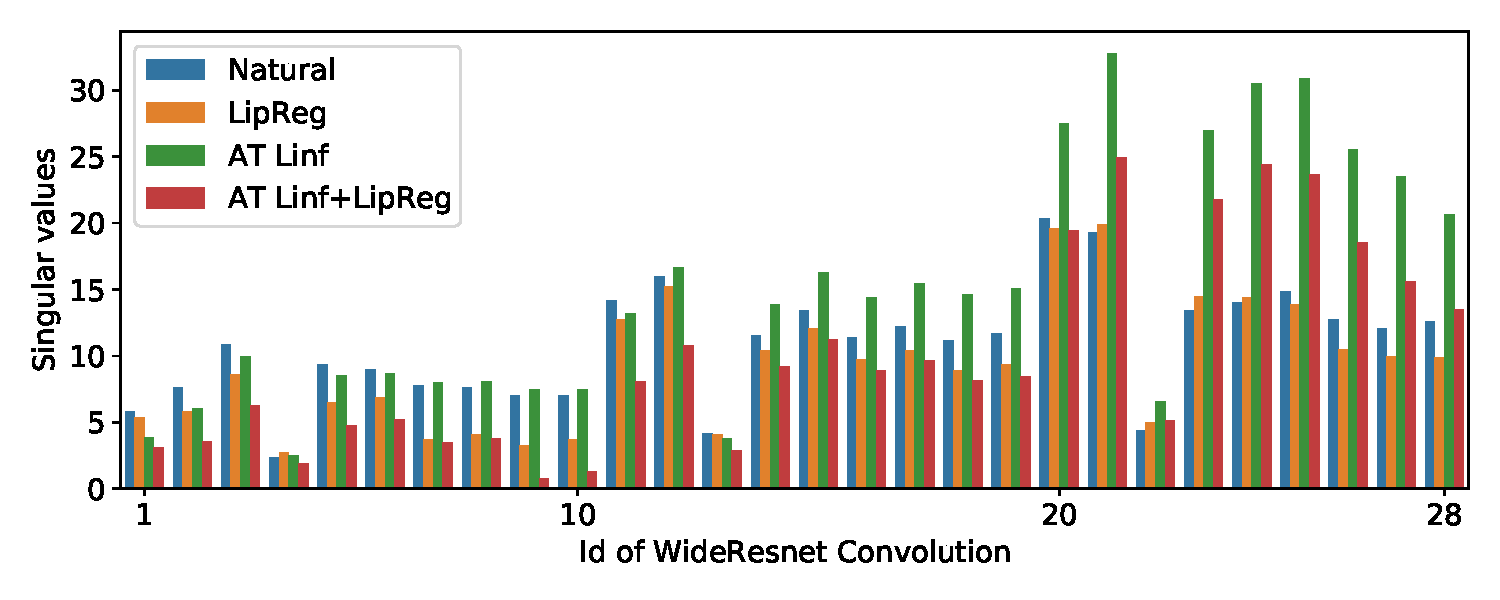
\includegraphics[scale=0.55]{figures/chapter4/singular_values.pdf}
%     \caption{This figure shows the maximal singular values of each convolution of a trained Wide ResNet on CIFAR10 dataset given different training scheme. The id 1 and 28 correspond to the first layer and last layer of the network.}
%     \label{figure:singular_values}
% \end{figure*}%
%
% Figure~\ref{figure:singular_values} shows the maximal singular values of each convolution of a trained Wide ResNet on CIFAR10 dataset given different training scheme. We can observe a small but clear decrease in the magnitude of the maximal singular values between Baseline and LipReg (blue and orange) on most of the convolution layers. A high increase of the maximal singular values appear with Adversarial Training. This is expected because the training scheme requires to the network to be a lot more expressive with the same number of parameters. We can observe that LipReg combined with AT have an important impact due on the singular value. 
%
%

  %%%%%%%%%%%%%%%%%%%%%%%%%%%%%%%%%%%%%%%%%%%%%%%%%%%%%%%%%%%%%%%%%%%%%%%%
\chapter{Conclusion}
\label{chapter:conlusion}
%%%%%%%%%%%%%%%%%%%%%%%%%%%%%%%%%%%%%%%%%%%%%%%%%%%%%%%%%%%%%%%%%%%%%%%%

xxx


  % \appendix
  % \input{sources/ap1-randomized_inference}
  % \input{sources/ap2-advocating_for_multiple_defense_strategies}

  \printbibliography[title=References]


\end{document}
